\documentclass[aspectratio=169]{beamer}
% ============================================================================
% HEC Montréal MBA -- ECON50803: Macroeconomic Environment
% Shared Beamer Preamble
% ============================================================================

% --- Theme and base settings ------------------------------------------------
\usetheme{default}
\setbeamersize{text margin left=1.2cm, text margin right=1.2cm}

% --- Fonts ------------------------------------------------------------------
% Sans-serif throughout for a business look (comment out FiraSans if unavailable)
\usepackage[sfdefault,light]{FiraSans}
\usepackage{FiraMono}
\usepackage[T1]{fontenc}
\usepackage[utf8]{inputenc}
\setbeamerfont{title}{series=\bfseries, size=\Large}
\setbeamerfont{frametitle}{series=\bfseries, size=\large}
\setbeamerfont{framesubtitle}{series=\mdseries, size=\normalsize}

% --- Colors -----------------------------------------------------------------
\definecolor{HECnavy}{HTML}{002855}
\definecolor{HECgreen}{HTML}{26d07c}
\definecolor{HECcoral}{HTML}{ff585d}
\definecolor{HECtext}{HTML}{2D3748}
\definecolor{HECgray}{HTML}{94A3B8}
\definecolor{HEClightgray}{HTML}{F1F5F9}
\definecolor{HEClightblue}{HTML}{E8EDF3}

% Beamer color assignments
\setbeamercolor{normal text}{fg=HECtext}
\setbeamercolor{title}{fg=HECnavy}
\setbeamercolor{frametitle}{fg=HECnavy}
\setbeamercolor{structure}{fg=HECnavy}
\setbeamercolor{background canvas}{bg=white}
\setbeamercolor{alerted text}{fg=HECcoral}
\setbeamercolor{example text}{fg=HECgreen}
\hypersetup{colorlinks, linkcolor=HECnavy, urlcolor=HECnavy, citecolor=HECtext}

% --- Navigation and chrome --------------------------------------------------
\setbeamertemplate{navigation symbols}{}

% Frame title: bold text with a thin accent line
\setbeamertemplate{frametitle}{%
   \vspace{0.25cm}%
   {\usebeamerfont{frametitle}\usebeamercolor[fg]{frametitle}\insertframetitle}%
   \ifx\insertframesubtitle\empty\else%
      \\[2pt]{\usebeamerfont{framesubtitle}\textcolor{HECgray}{\insertframesubtitle}}%
   \fi%
   \\[-4pt]\textcolor{HECgreen}{\rule{2.5cm}{1.5pt}}%
   \\[-2pt]%
}

% Footer: course name left, slide number right, thin rule above
\setbeamertemplate{footline}{%
   \vspace{-0.1cm}%
   \hbox to \paperwidth{%
      \hspace{1.2cm}%
      \textcolor{HEClightgray}{\rule{0.84\paperwidth}{0.4pt}}%
      \hspace{1.2cm}%
   }%
   \vspace{0.05cm}%
   \hbox to \paperwidth{%
      \hspace{1.2cm}%
      {\scriptsize\textcolor{HECgray}{ECON 50803\enspace\textbar\enspace Environnement macroéconomique}}%
      \hfill%
      {\scriptsize\textcolor{HECgray}{\insertframenumber}}%
      \hspace{1.2cm}%
   }%
   \vspace{0.15cm}%
}

% --- Itemize/enumerate styling ----------------------------------------------
\setbeamertemplate{itemize item}{\textcolor{HECnavy}{$\bullet$}}
\setbeamertemplate{itemize subitem}{\textcolor{HECgray}{$\bullet$}}
\setbeamertemplate{itemize subsubitem}{\textcolor{HECgray}{\scalebox{0.6}{$\blacktriangleright$}}}
\setbeamertemplate{enumerate item}{\textcolor{HECnavy}{\bfseries\insertenumlabel.}}
\setbeamertemplate{enumerate subitem}{\textcolor{HECgray}{\insertsubenumlabel.}}

% --- Packages ---------------------------------------------------------------
\usepackage{
   tikz, caption, subcaption, ragged2e, amsmath, bm,
   makecell, threeparttable, booktabs, mathtools,
   multirow, calc, hyperref, tabularx, colortbl,
   transparent, tcolorbox, xcolor, graphicx
}
\usepackage[round]{natbib}
\usetikzlibrary{decorations.pathreplacing, decorations.markings, calc, arrows.meta, positioning}
\usepackage[absolute,overlay]{textpos}
\captionsetup[figure]{labelformat=empty, font=small, textfont=it}
\captionsetup[table]{labelformat=empty, font=small}
\setlength{\belowcaptionskip}{0cm}
\apptocmd{\frame}{}{\justifying}

% --- Paths ------------------------------------------------------------------
\graphicspath{{../Figures/}}
\newcommand*\includetables[1]{\input{../Tables/#1.tex}}

% --- Mathematical commands --------------------------------------------------
\DeclareMathOperator*{\argmax}{arg\,max}
\newcommand{\partialof}[2]{\frac{\partial #1}{\partial #2}}
\newcommand{\totalof}[2]{\frac{\text{d}#1}{\text{d}#2}}
\newcommand{\pctchg}[1]{\%\Delta #1}
\newcommand{\smallquad}{\hspace{0.5em}}

% --- Resize equation command ------------------------------------------------
\newcommand{\resizeeq}[2]{\resizebox{#2\hsize}{!}{$#1$}}

% ============================================================================
% CUSTOM SLIDE TYPES
% ============================================================================

% --- Title slide (call with \titleframe) ------------------------------------
\newcommand{\titleframe}{%
   {\setbeamertemplate{footline}{}%
   \begin{frame}[plain]
      \begin{tikzpicture}[remember picture, overlay]
         % Navy accent bar on the left
         \fill[HECnavy] (current page.north west) rectangle
            ([xshift=0.6cm]current page.south west);
         % Green accent line
         \fill[HECgreen] ([xshift=0.6cm]current page.north west) rectangle
            ([xshift=0.65cm]current page.south west);
      \end{tikzpicture}
      \vspace{1cm}
      \hspace{0.6cm}%
      \begin{minipage}{0.85\textwidth}
         {\usebeamerfont{title}\usebeamercolor[fg]{title}\inserttitle}
         \\[12pt]
         \textcolor{HECgreen}{\rule{3cm}{2pt}}
         \\[12pt]
         {\large\textcolor{HECgray}{\insertauthor}}
         \\[6pt]
         {\normalsize\textcolor{HECgray}{\insertdate}}
      \end{minipage}
      \vfill
      \hspace{0.6cm}%
      {\footnotesize\textcolor{HECgray}{HEC Montréal \enspace\textbar\enspace MBA}}
      \vspace{0.5cm}
   \end{frame}}%
}

% --- Section divider slide --------------------------------------------------
\newcommand{\sectionframe}[1]{%
   {\setbeamertemplate{footline}{}%
   \begin{frame}[plain]
      \begin{tikzpicture}[remember picture, overlay]
         \fill[HECnavy] ([shift={(-1pt,1pt)}]current page.north west) rectangle
            ([shift={(1pt,-1pt)}]current page.south east);
         \node[anchor=center] at (current page.center) {%
            \begin{minipage}{0.8\paperwidth}
               \centering
               {\LARGE\bfseries\textcolor{white}{#1}}
               \\[12pt]
               \textcolor{HECgreen}{\rule{3cm}{2pt}}
            \end{minipage}
         };
      \end{tikzpicture}
   \end{frame}}%
}

% ============================================================================
% CUSTOM BOX ENVIRONMENTS
% ============================================================================

% Key Insight (green accent)
\newtcolorbox{keyinsight}[1][Point clé]{%
   colback=HECgreen!5,
   colframe=HECgreen,
   boxrule=0pt,
   leftrule=3pt,
   arc=8pt,
   title={\textcolor{HECgreen}{\bfseries #1}},
   coltitle=HECgreen,
   fonttitle=\bfseries,
   attach title to upper={\\[4pt]},
   left=10pt, right=10pt, top=6pt, bottom=6pt
}

% Business Implication (navy accent)
\newtcolorbox{bizimplication}[1][Implication d'affaires]{%
   colback=HECnavy!5,
   colframe=HECnavy,
   boxrule=0pt,
   leftrule=3pt,
   arc=8pt,
   title={\textcolor{HECnavy}{\bfseries #1}},
   coltitle=HECnavy,
   fonttitle=\bfseries,
   attach title to upper={\\[4pt]},
   left=10pt, right=10pt, top=6pt, bottom=6pt
}

% Warning / Important (coral accent)
\newtcolorbox{warning}[1][Important]{%
   colback=HECcoral!5,
   colframe=HECcoral,
   boxrule=0pt,
   leftrule=3pt,
   arc=8pt,
   title={\textcolor{HECcoral}{\bfseries #1}},
   coltitle=HECcoral,
   fonttitle=\bfseries,
   attach title to upper={\\[4pt]},
   left=10pt, right=10pt, top=6pt, bottom=6pt
}

% Definition (gray background)
\newtcolorbox{defbox}[1][Définition]{%
   colback=HEClightgray,
   colframe=HEClightgray,
   boxrule=0pt,
   leftrule=3pt,
   arc=8pt,
   left=10pt, right=10pt, top=6pt, bottom=6pt,
   title={\textcolor{HECnavy}{\bfseries #1}},
   coltitle=HECnavy,
   fonttitle=\bfseries,
   attach title to upper={\\[4pt]}
}

% In-Class Exercise (coral accent)
\newtcolorbox{exercise}[1][Exercice]{%
   colback=HECcoral!5,
   colframe=HECcoral,
   boxrule=0pt,
   leftrule=3pt,
   arc=8pt,
   title={\textcolor{HECcoral}{\bfseries #1}},
   coltitle=HECcoral,
   fonttitle=\bfseries,
   attach title to upper={\\[4pt]},
   left=10pt, right=10pt, top=6pt, bottom=6pt
}

% ============================================================================
% NEWSPAPER HEADLINES SLIDE TEMPLATE
% ============================================================================
% Usage: inside a frame, open a tikzpicture[remember picture, overlay], then:
%   \setcounter{newshl}{0}
%   \newsheadline{Newspaper Name}{``Headline text''}   % up to 6 entries
%   \headlinesoverlay{Large overlay text}               % optional 2nd slide
%
% Headlines are auto-positioned in a 2×3 staggered grid (left/right alternating).
%
% Logo support: place PNG files in Figures/logos/ (e.g., ft.png, economist.png).
% Use the optional argument to specify the logo file (without extension):
%   \newsheadline[ft]{Financial Times}{Headline text}   % logo + bold headline
%   \newsheadline{The Economist}{``Headline text''}      % text-only fallback

\newcounter{newshl}

\newcommand{\newsheadline}[3][]{%
   % #1 = optional logo file key (e.g., ft → logos/ft.png)
   % #2 = newspaper name (text fallback when no logo)
   % #3 = headline text
   \stepcounter{newshl}%
   \pgfmathsetmacro{\hlrow}{int((\thenewshl-1)/2)}%
   \pgfmathsetmacro{\hlcol}{int(mod(\thenewshl-1,2))}%
   \pgfmathsetmacro{\hlx}{0.8 + \hlcol * 7.8}%
   \pgfmathsetmacro{\hly}{-1.5 - \hlrow * 2.0}%
   \node[anchor=north west]
      at ([shift={(\hlx cm,\hly cm)}]current page.north west) {%
      \ifx\\#1\\%
         \begin{minipage}[t]{5.8cm}%
            \textbf{\textcolor{HECgray}{\footnotesize\MakeUppercase{#2}}}%
            \\[-1pt]%
            {\small\itshape #3}%
         \end{minipage}%
      \else%
         \begin{minipage}[c]{1.2cm}%
            \includegraphics[height=1.2cm]{logos/#1}%
         \end{minipage}%
         \hspace{6pt}%
         \begin{minipage}[c][1.2cm][c]{4.3cm}%
            \raggedright{\small\textcolor{HECtext!75}{#3}}%
         \end{minipage}%
      \fi%
   };%
}

\newcommand{\headlinesoverlay}[1]{%
   \only<2>{%
      \fill[white, opacity=0.85]
         (current page.south west) rectangle (current page.north east);%
      \node[anchor=center] at ([yshift=-0.5cm]current page.center) {%
         {\fontsize{36}{44}\selectfont\bfseries\textcolor{HECnavy}{#1}}%
      };%
   }%
}

% ============================================================================
% NAVIGATION BUTTONS (optional, for bottom-of-slide section nav)
% ============================================================================

\newlength{\buttonwidth}
\newlength{\currentxpos}
\setlength{\currentxpos}{1.2cm}
\newlength{\buttonsep}
\setlength{\buttonsep}{0.05cm}

\newcommand{\mybutton}[2]{%
   \settowidth{\buttonwidth}{#1}%
   \begin{textblock*}{\buttonwidth + 2ex}(\currentxpos, \paperheight - 2.5em)
      \hyperlink{#2}{\beamerbutton{#1}}
   \end{textblock*}%
   \addtolength{\currentxpos}{\buttonwidth + \buttonsep}%
}

% ============================================================================
% BACKUP SLIDES SUPPORT
% ============================================================================

\newcommand{\backupbegin}{%
   \newcounter{finalframe}%
   \setcounter{finalframe}{\value{framenumber}}%
}
\newcommand{\backupend}{%
   \setcounter{framenumber}{\value{finalframe}}%
}


\title{Croissance de long terme}
\author{Jean-Félix Brouillette}
\date{Séance 2}

\begin{document}

% ============================================================================
\titleframe
% ============================================================================

% --- Opening Hook: Shanghai 1987 ---
{
\setbeamertemplate{footline}{}
\begin{frame}[plain]
   \begin{tikzpicture}[remember picture, overlay]
      \node[anchor=center, inner sep=0pt] at (current page.center) {%
         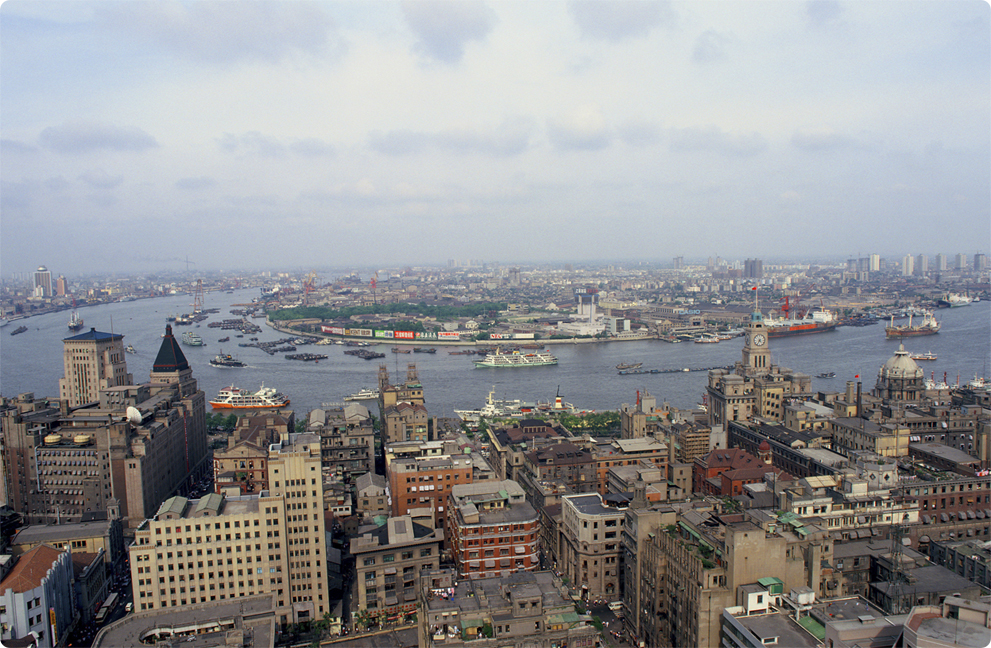
\includegraphics[width=\paperwidth, height=\paperheight, keepaspectratio]{shanghai_1987.png}%
      };
      \node[anchor=south west, fill=black, fill opacity=0.5, text opacity=1, inner sep=6pt]
         at ([shift={(0.3cm,0.3cm)}]current page.south west)
         {\large\bfseries\textcolor{white}{Shanghai, 1987}};
   \end{tikzpicture}
\end{frame}
}

% --- Opening Hook: Shanghai 2013 ---
{
\setbeamertemplate{footline}{}
\begin{frame}[plain]
   \begin{tikzpicture}[remember picture, overlay]
      \node[anchor=center, inner sep=0pt] at (current page.center) {%
         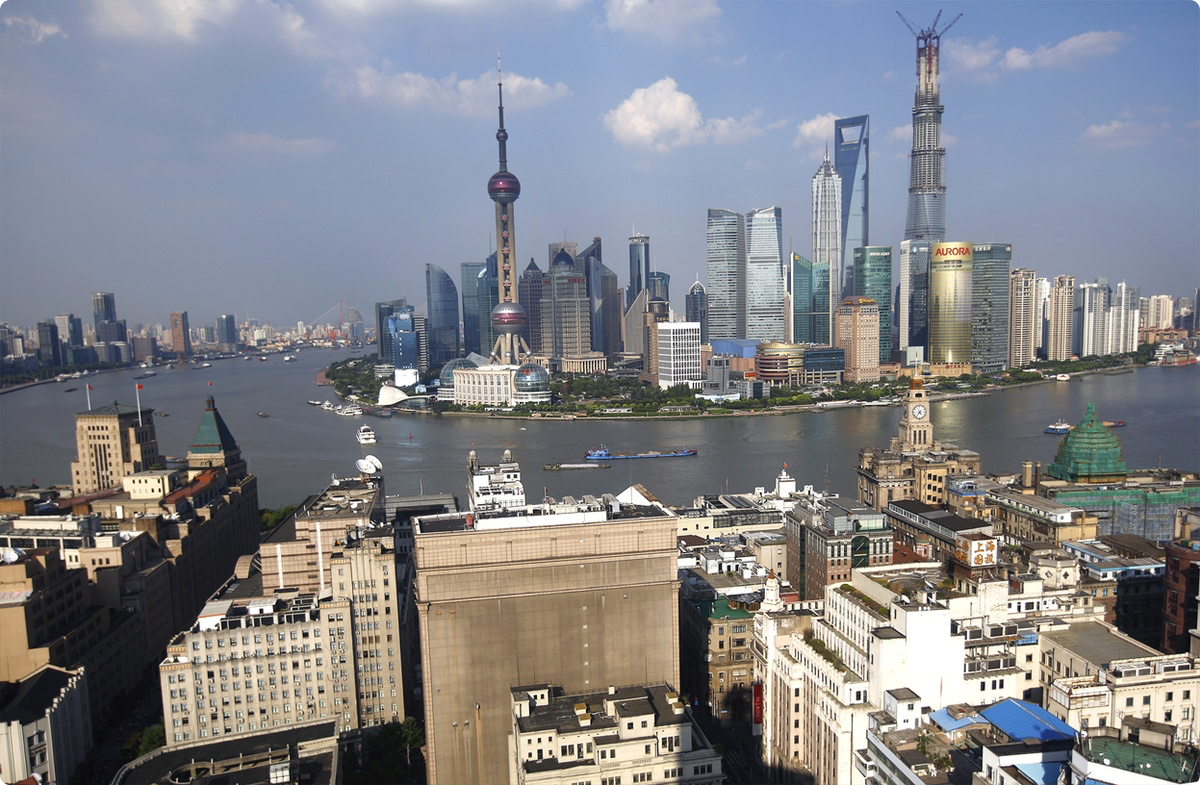
\includegraphics[width=\paperwidth, height=\paperheight, keepaspectratio]{shanghai_2013.png}%
      };
      \node[anchor=south west, fill=black, fill opacity=0.5, text opacity=1, inner sep=6pt]
         at ([shift={(0.3cm,0.3cm)}]current page.south west)
         {\large\bfseries\textcolor{white}{Shanghai, 2013}};
   \end{tikzpicture}
\end{frame}
}

% --- Opening Hook: Manhattan ---
\begin{frame}{Manhattan, de 1876 à 2013}
   % TODO: Replace placeholder with 4-era photo montage (Vincent sl.27 or similar)
   \begin{tcolorbox}[
      colback=HEClightgray, colframe=HEClightgray, arc=8pt,
      width=\textwidth, height=0.7\textheight,
      halign=center, valign=center
   ]
      {\large\itshape\textcolor{HECgray}{Photo montage : Manhattan à travers les époques}}\\[6pt]
      {\small\textcolor{HECgray}{1876 -- 1932 -- 1988 -- 2013}}
   \end{tcolorbox}
\end{frame}

% ============================================================================
\begin{frame}{Plan}
   \begin{enumerate}
      \setlength\itemsep{0.25cm}
      \item \textbf{La croissance est un phénomène récent}
      \item La fonction de production
      \item Décomposer la croissance
      \item Le modèle de Solow
      \item Convergence
      \item Le vrai moteur de la croissance
      \item Le casse-tête canadien de la productivité
      \item Croissance et environnement
   \end{enumerate}
\end{frame}

% ============================================================================
\sectionframe{La croissance est un phénomène récent}
% ============================================================================

\begin{frame}{La croissance est un phénomène récent}
   \begin{figure}
      \centering
      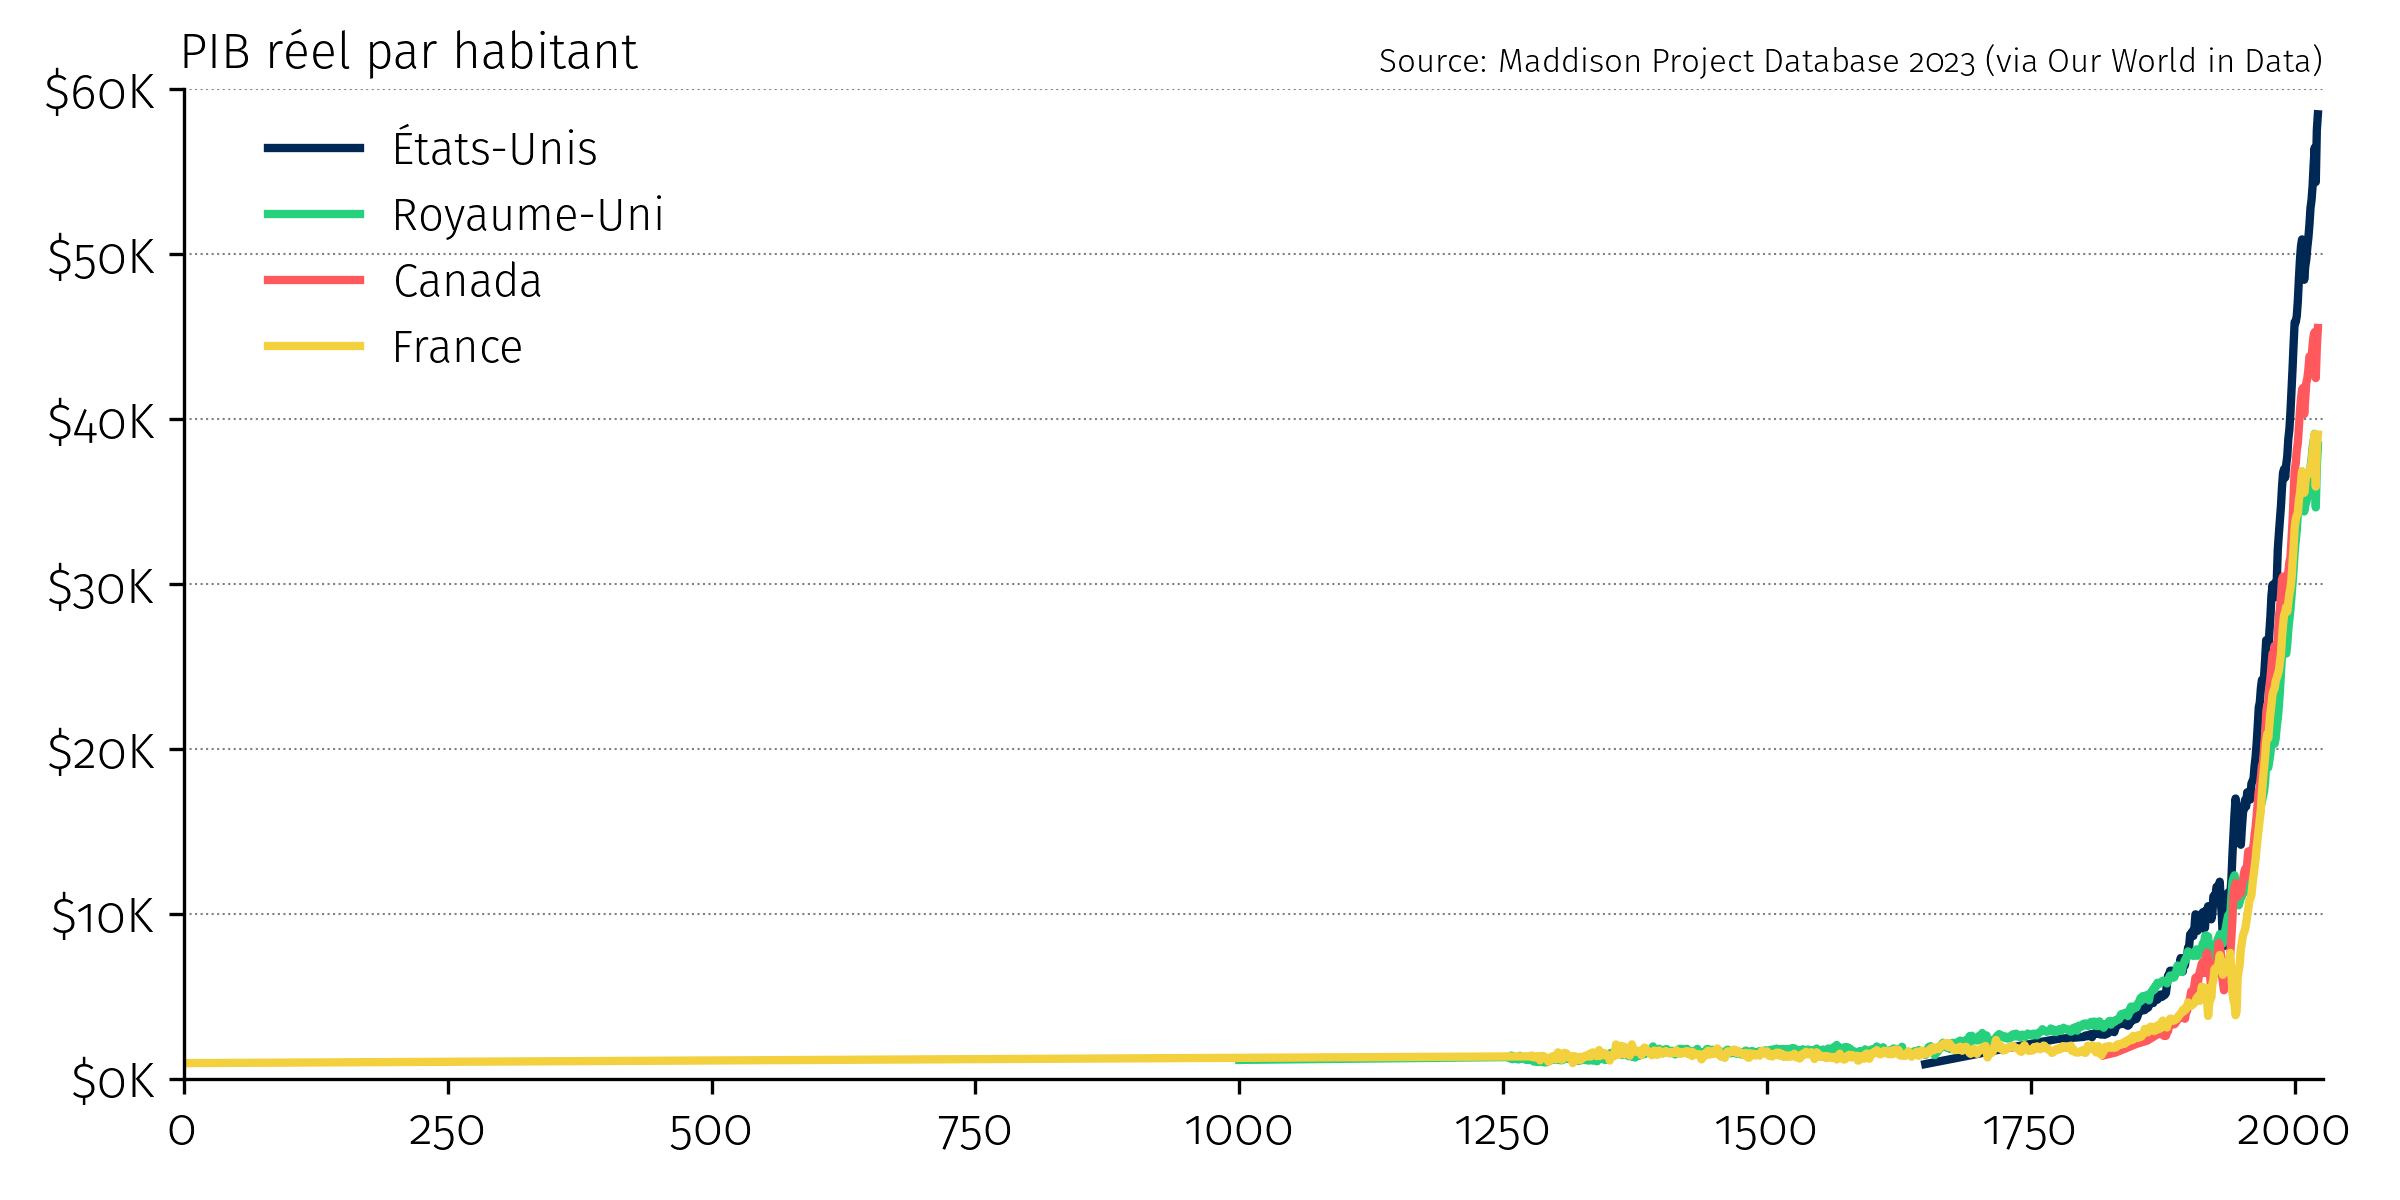
\includegraphics[width=0.9\textwidth]{hockey_stick_world.png}
   \end{figure}
\end{frame}

\begin{frame}{Des expériences très différentes}
   \begin{figure}
      \centering
      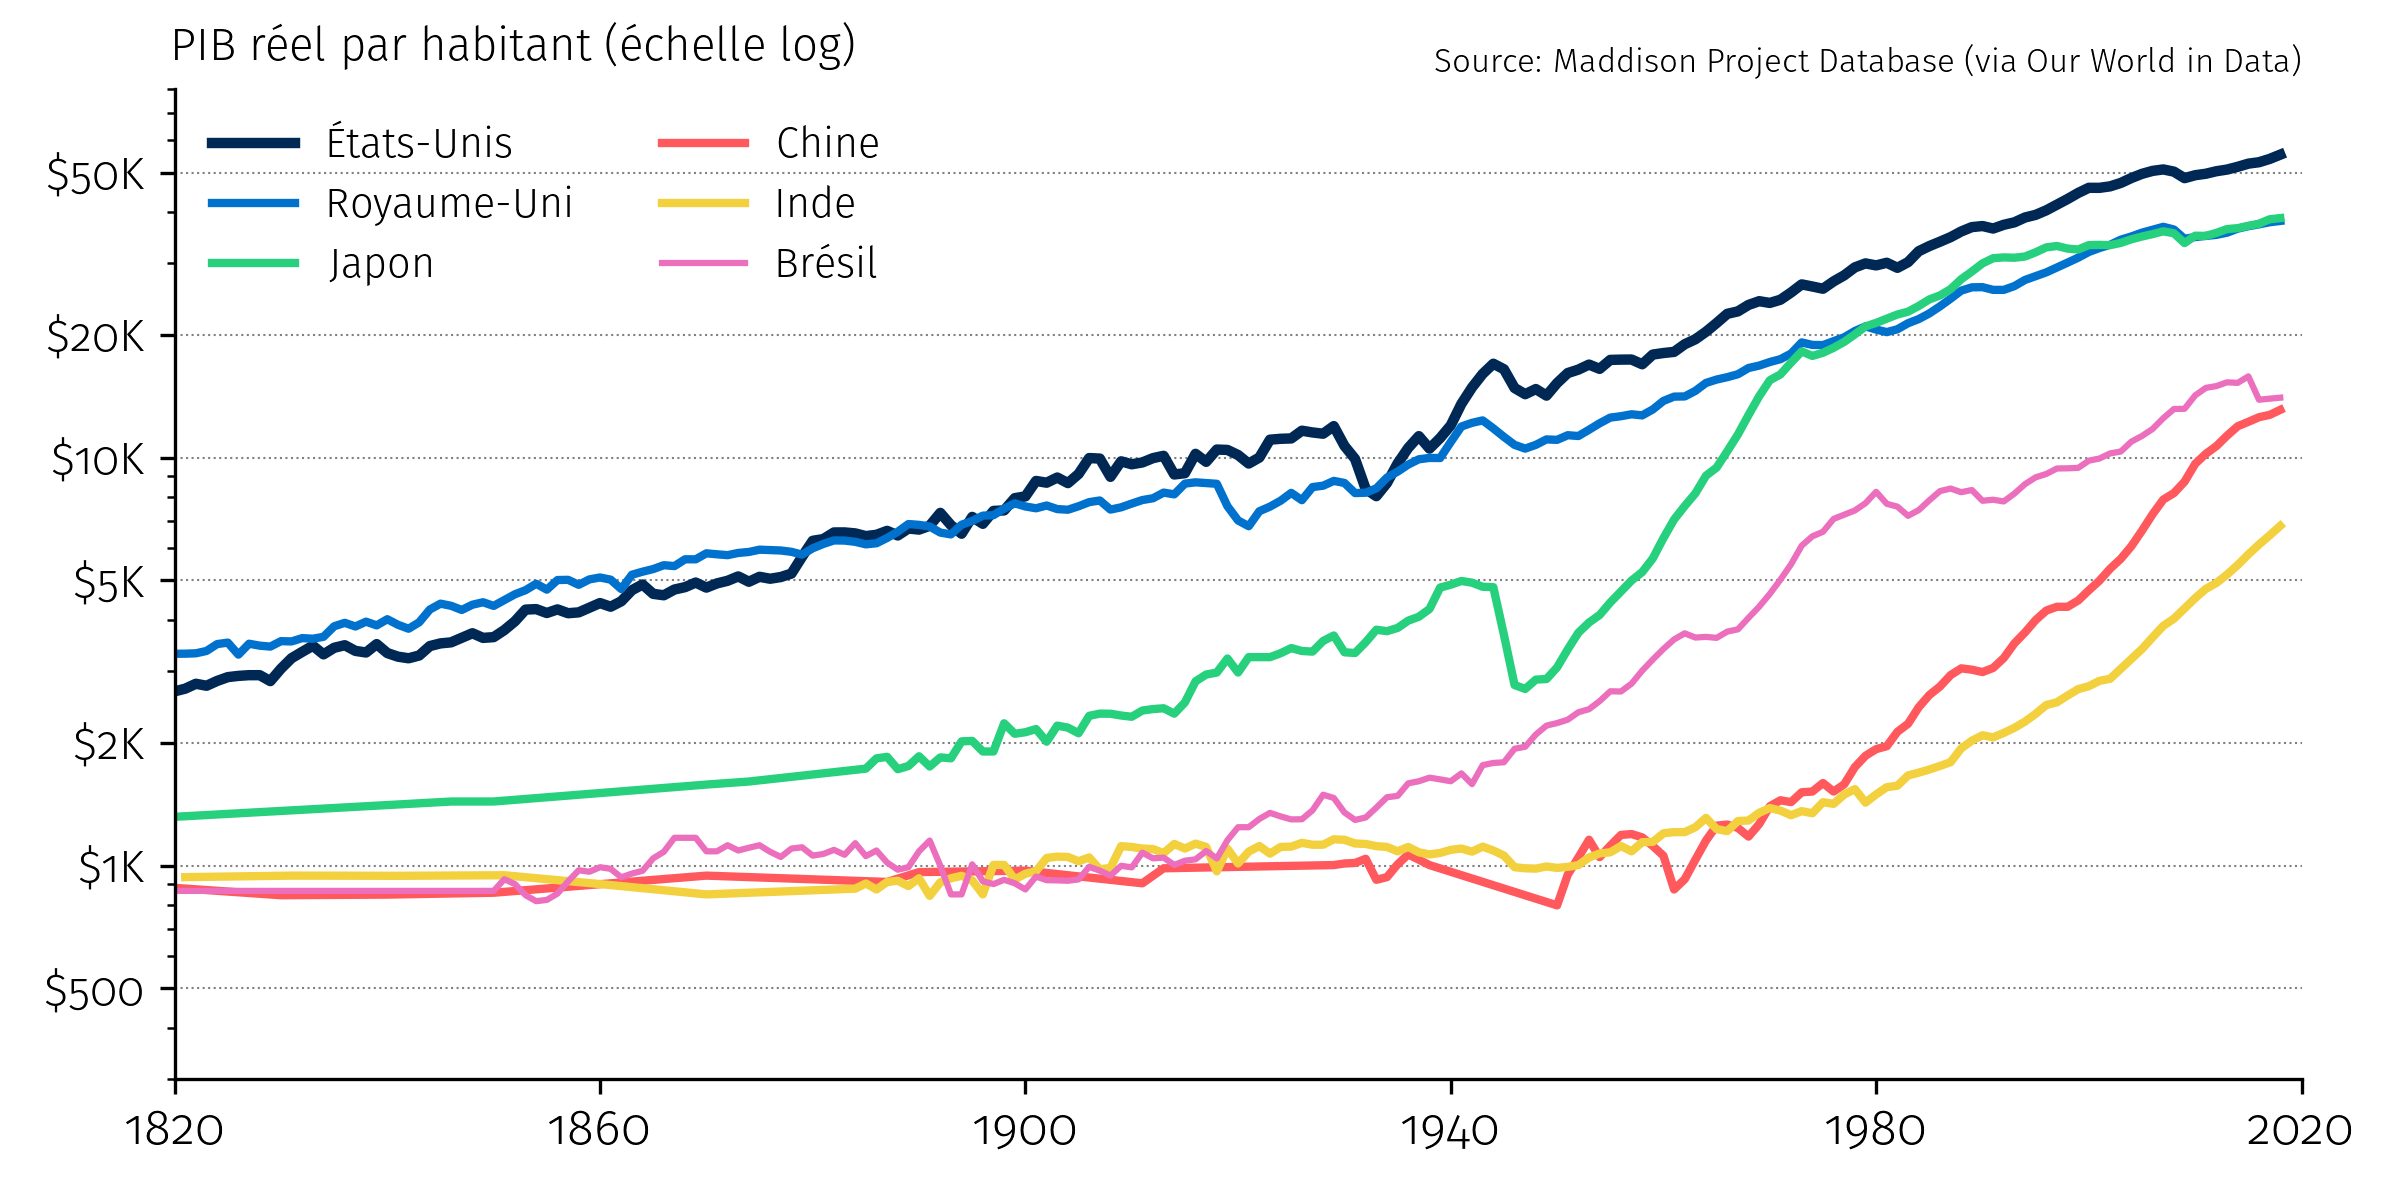
\includegraphics[width=0.9\textwidth]{regional_divergence.png}
   \end{figure}
\end{frame}

\begin{frame}[t]{Trois faits stylisés sur la croissance}
   \small
   L'économiste Nicholas Kaldor a identifié des régularités empiriques remarquables :
   \vspace{0.3cm}
   \begin{enumerate}
      \setlength\itemsep{0.3cm}
      \item Le \textbf{PIB par habitant} croît à un rythme approximativement \textbf{constant} dans les pays avancés (en échelle logarithmique : une droite)
      \item Le ratio \textbf{capital/PIB} ($K/Y$) est approximativement \textbf{constant} à long terme
      \item Les \textbf{parts du revenu} versées au capital ($\sim$30\,\%) et au travail ($\sim$70\,\%) sont approximativement \textbf{constantes}
   \end{enumerate}
   \vspace{0.2cm}
   \begin{keyinsight}
      Tout bon modèle de croissance devrait être capable de reproduire ces régularités.
   \end{keyinsight}
\end{frame}

\begin{frame}[t]{Croissance et stratégies d'affaires}
   \small
   La croissance de long terme façonne les opportunités d'affaires :
   \vspace{0.2cm}
   \begin{itemize}
      \setlength\itemsep{0.15cm}
      \item \textbf{Pénétration de marché :} taille du marché, démographie, distribution des revenus
      \item \textbf{Investissement direct étranger :} infrastructure, productivité, environnement politique
      \item \textbf{Chaînes d'approvisionnement :} main-d'œuvre qualifiée, stabilité, logistique
   \end{itemize}
   \vspace{0.15cm}
   \begin{bizimplication}
      Comprendre les \textbf{déterminants} de la croissance vous aide à identifier les marchés porteurs, à évaluer les risques pays et à anticiper les tendances à long terme.
   \end{bizimplication}
\end{frame}

\begin{frame}{D'où vient la croissance?}
   La croissance économique transforme les sociétés de manière spectaculaire\ldots
   \vspace{0.3cm}

   Mais \textbf{d'où vient-elle?}
   \vspace{0.3cm}
   \begin{itemize}
      \setlength\itemsep{0.2cm}
      \item Quels sont les \textbf{ingrédients} de la production?
      \item Comment ces ingrédients se \textbf{combinent-ils?}
      \item Pourquoi certains pays en ont-ils \textbf{plus} que d'autres?
   \end{itemize}
   \vspace{0.3cm}
   Pour répondre, il nous faut un modèle de production $\to$ la \textbf{fonction de production}
\end{frame}

% ============================================================================
\begin{frame}{Plan}
   \begin{enumerate}
      \setlength\itemsep{0.25cm}
      \item {\color{gray!50}La croissance est un phénomène récent}
      \item \textbf{La fonction de production}
      \item Décomposer la croissance
      \item Le modèle de Solow
      \item Convergence
      \item Le vrai moteur de la croissance
      \item Le casse-tête canadien de la productivité
      \item Croissance et environnement
   \end{enumerate}
\end{frame}

% ============================================================================
\sectionframe{La fonction de production}
% ============================================================================

\begin{frame}[t]{Qu'est-ce qui détermine la production?}
   \small
   \begin{columns}[T]
      \begin{column}{0.55\textwidth}
         La production dépend de trois ingrédients :
         \vspace{0.15cm}
         \begin{itemize}
            \setlength\itemsep{0.15cm}
            \item $K$ = \textbf{Capital} : machines, équipements, bâtiments, infrastructures
            \item $N$ = \textbf{Travail} : heures travaillées, nombre d'employés
            \item $A$ = \textbf{Productivité} (PTF) : technologie, savoir-faire, organisation
         \end{itemize}
         \vspace{0.15cm}
         \begin{defbox}[Fonction de production]
            $Y = A \cdot F(K, N)$\\[4pt]
            Comment les intrants se combinent pour produire $Y$
         \end{defbox}
      \end{column}
      \begin{column}{0.42\textwidth}
         \vspace{0.2cm}
         \centering
         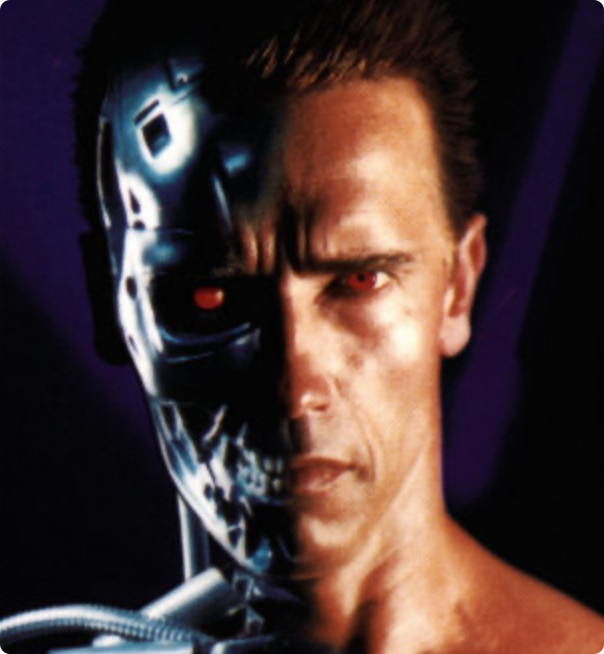
\includegraphics[width=\textwidth, keepaspectratio]{terminator.png}\\[4pt]
         {\footnotesize\textcolor{HECgray}{Capital ($K$) + Travail ($N$)}}
      \end{column}
   \end{columns}
\end{frame}

\begin{frame}[t]{La fonction Cobb-Douglas}
   La forme fonctionnelle la plus utilisée en macroéconomie :
   \vspace{0.2cm}
   \begin{equation*}
      \boxed{Y = A \cdot K^{\alpha} \cdot N^{1-\alpha}} \qquad \text{avec } \alpha \approx 0{,}3
   \end{equation*}
   \vspace{0.1cm}
   \begin{itemize}
      \setlength\itemsep{0.15cm}
      \item $A$ = \textbf{productivité totale des facteurs} (PTF)
      \item $K^{\alpha}$ = contribution du capital (part $\alpha \approx 30\,\%$ du revenu)
      \item $N^{1-\alpha}$ = contribution du travail (part $1-\alpha \approx 70\,\%$)
   \end{itemize}
   \vspace{0.15cm}
   \begin{keyinsight}
      Les exposants $\alpha$ et $1-\alpha$ correspondent aux \textbf{parts du revenu} versées au capital et au travail --- exactement ce que Kaldor a observé!
   \end{keyinsight}
\end{frame}

\begin{frame}{Rendements décroissants}
   \begin{columns}[c]
      \begin{column}{0.55\textwidth}
         \begin{figure}
            \centering
            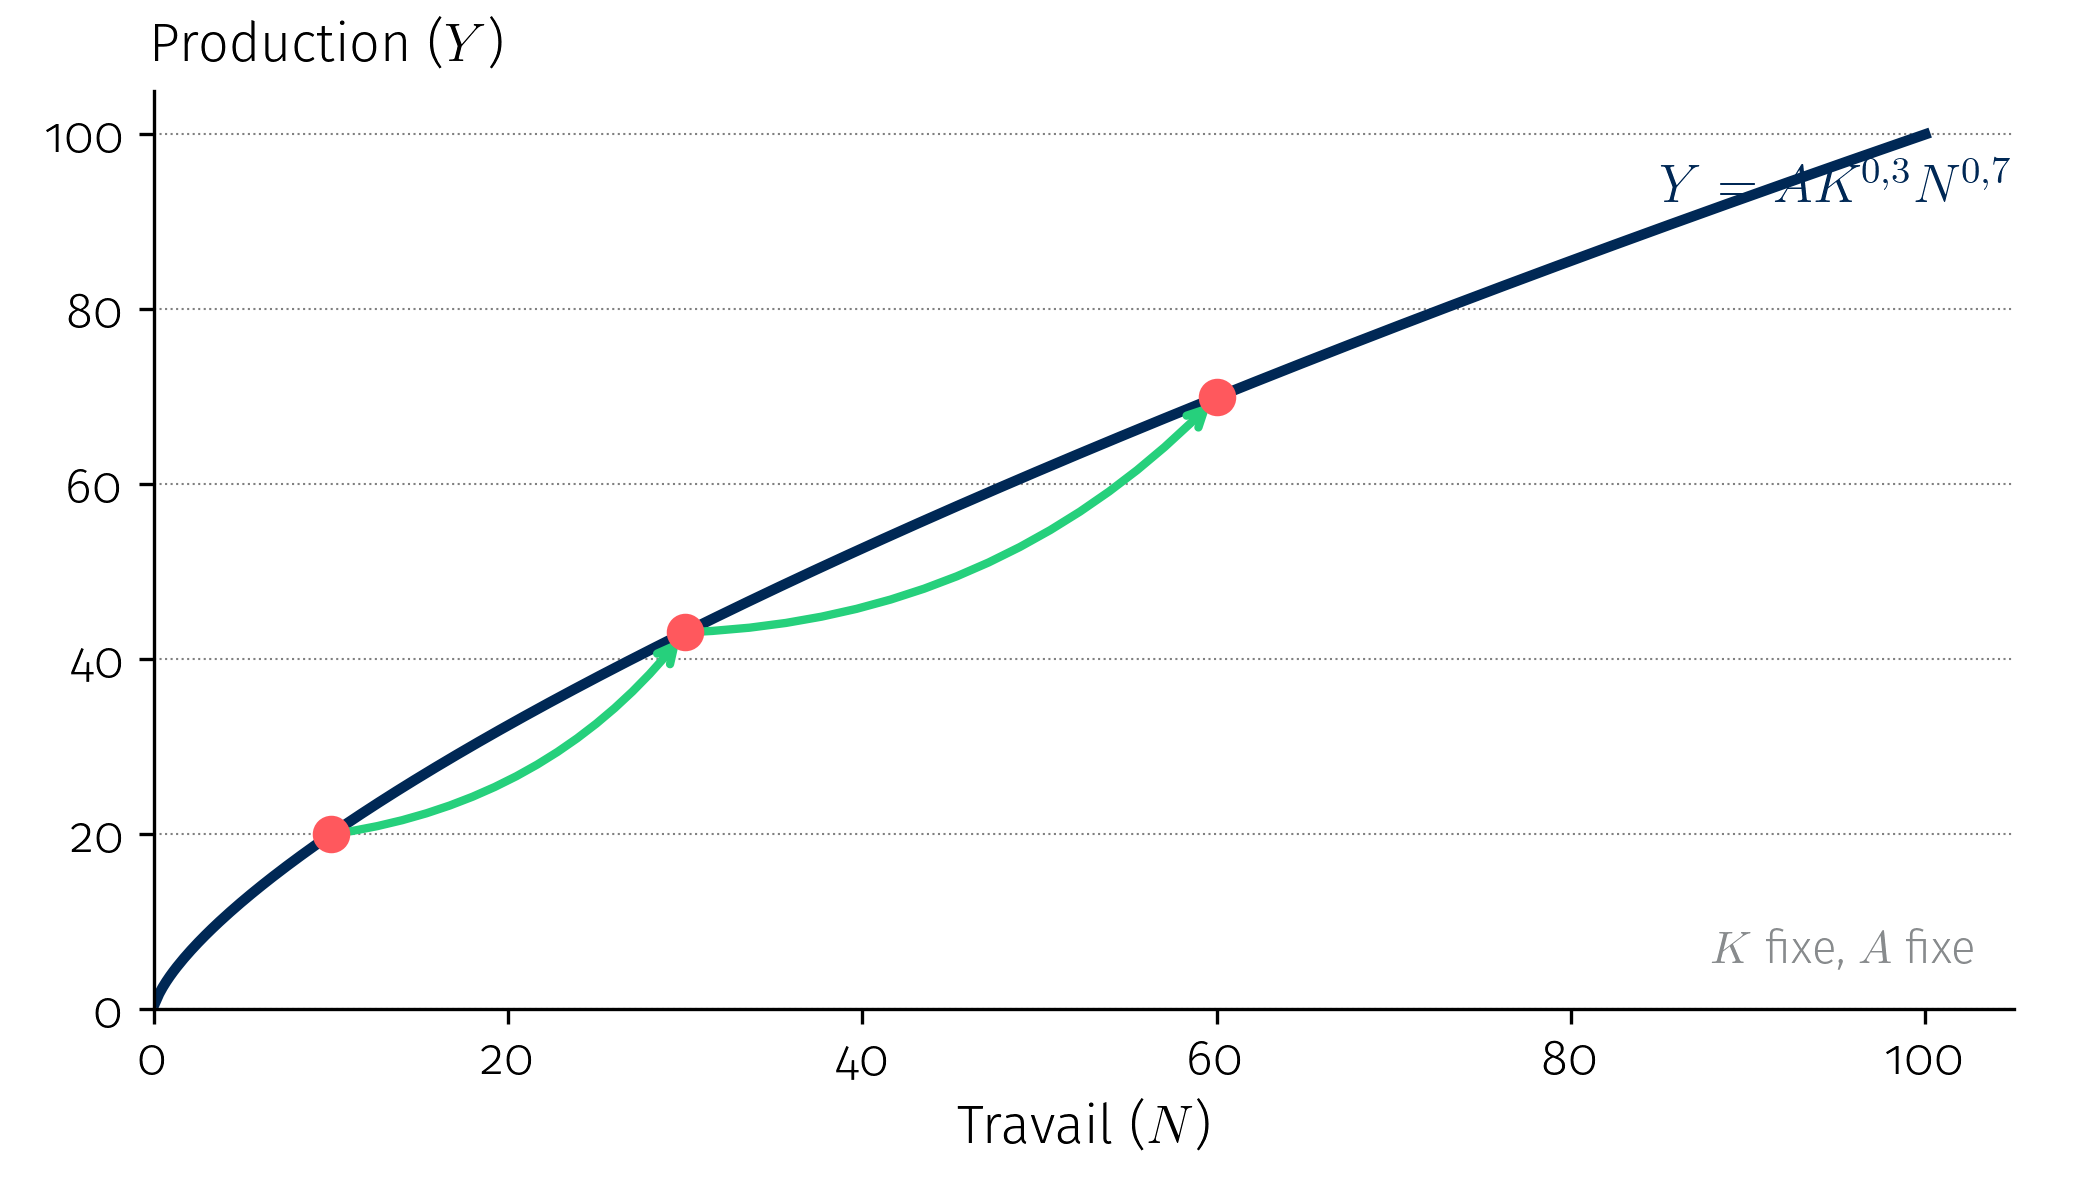
\includegraphics[width=\textwidth]{production_function.png}
         \end{figure}
      \end{column}
      \begin{column}{0.42\textwidth}
         À capital fixe, chaque travailleur supplémentaire \textbf{ajoute de moins en moins} à la production.
         \vspace{0.2cm}

         \textbf{Analogie :} mettre 10 cuisiniers dans une seule cuisine --- le 10\textsuperscript{e} est beaucoup moins productif que le 1\textsuperscript{er}!
         \vspace{0.2cm}

         \begin{warning}[Attention]
            Plus de $N$ $\to$ plus de $Y$, mais à un rythme \textbf{décroissant}
         \end{warning}
      \end{column}
   \end{columns}
\end{frame}

\begin{frame}[t]{Rendements d'échelle constants}
   Si on \textbf{double} tous les intrants, la production \textbf{double} :
   \vspace{0.1cm}
   \begin{equation*}
      A \cdot (2K)^{\alpha} \cdot (2N)^{1-\alpha} = 2^{\alpha} \cdot 2^{1-\alpha} \cdot A K^{\alpha} N^{1-\alpha} = 2Y
   \end{equation*}
   \vspace{0.1cm}
   \textbf{Intuition :} cloner l'usine avec les mêmes machines et le même nombre de travailleurs $\to$ on produit exactement le double.
   \vspace{0.2cm}
   \begin{keyinsight}
      La \textbf{taille} d'un pays ne détermine pas son niveau de vie. Ce qui compte, c'est le capital \textbf{par travailleur} ($K/N$) et la productivité ($A$).
   \end{keyinsight}
\end{frame}

\begin{frame}[t]{La PTF : le facteur mystérieux}
   \small
   La \textbf{productivité totale des facteurs} ($A$) capte tout ce qui n'est pas $K$ ou $N$ :
   \vspace{0.15cm}
   \begin{itemize}
      \setlength\itemsep{0.1cm}
      \item Technologie et innovation
      \item Qualité des institutions (droits de propriété, état de droit)
      \item Qualité du management et de l'organisation
      \item Éducation et capital humain
      \item Infrastructure publique
   \end{itemize}
   \vspace{0.15cm}
   C'est un \textbf{résidu} : tout ce que $K$ et $N$ ne peuvent pas expliquer.
   \vspace{0.1cm}
   \begin{defbox}
      \guillemotleft~La productivité totale des facteurs est une mesure de notre ignorance.~\guillemotright
      \hfill {\small --- Moses Abramovitz (1956)}
   \end{defbox}
\end{frame}

\begin{frame}[t]{Exercice : propriétés de la Cobb-Douglas}
   \begin{exercise}
      Soit $Y = A K^{0{,}3} N^{0{,}7}$.
      \vspace{0.15cm}
      \begin{enumerate}
         \setlength\itemsep{0.25cm}
         \item \textbf{Rendements décroissants :} Montrez que le produit marginal du travail ($\partial Y / \partial N$) diminue lorsque $N$ augmente (à $K$ fixe).
         \item \textbf{Rendements d'échelle constants :} Montrez que si on multiplie $K$ et $N$ par $\lambda$, la production est multipliée par $\lambda$.
         \item \textbf{Rôle de la productivité :} Si $A$ double, qu'arrive-t-il à $Y$?
      \end{enumerate}
   \end{exercise}
\end{frame}

% ============================================================================
\begin{frame}{Plan}
   \begin{enumerate}
      \setlength\itemsep{0.25cm}
      \item {\color{gray!50}La croissance est un phénomène récent}
      \item {\color{gray!50}La fonction de production}
      \item \textbf{Décomposer la croissance}
      \item Le modèle de Solow
      \item Convergence
      \item Le vrai moteur de la croissance
      \item Le casse-tête canadien de la productivité
      \item Croissance et environnement
   \end{enumerate}
\end{frame}

% ============================================================================
\sectionframe{Décomposer la croissance}
% ============================================================================

\begin{frame}[t]{Comptabilité de la croissance}
   On peut décomposer la croissance du PIB en contributions de chaque source :
   \vspace{0.2cm}
   \begin{defbox}[Décomposition de Solow]
      \begin{equation*}
         \underbrace{\pctchg{Y}}_{\text{croissance du PIB}} \;\approx\; \underbrace{\pctchg{A}}_{\text{productivité}} \;+\; \underbrace{0{,}3 \cdot \pctchg{K}}_{\text{capital}} \;+\; \underbrace{0{,}7 \cdot \pctchg{N}}_{\text{travail}}
      \end{equation*}
   \end{defbox}
   \vspace{0.1cm}
   \begin{itemize}
      \setlength\itemsep{0.1cm}
      \item On observe $\pctchg{Y}$, $\pctchg{K}$ et $\pctchg{N}$
      \item On \textbf{déduit} $\pctchg{A}$ comme résidu : $\pctchg{A} = \pctchg{Y} - 0{,}3 \cdot \pctchg{K} - 0{,}7 \cdot \pctchg{N}$
   \end{itemize}
\end{frame}

\begin{frame}[t]{Le miracle asiatique}
   \footnotesize
   \vspace{0.1cm}
   \begin{tcolorbox}[
      colback=white, colframe=HECnavy, colbacktitle=HECnavy,
      title=\textbf{Comptabilité de la croissance (1966--1990)}, fonttitle=\footnotesize, boxrule=0.5pt, arc=8pt,
      top=3pt, bottom=3pt, left=6pt, right=6pt
   ]
      \renewcommand{\arraystretch}{1.2}
      \centering
      \begin{tabularx}{\linewidth}{X r r r r}
         \rowcolor{HECnavy!10}
         \textbf{Pays} & \textbf{$\pctchg{Y}$} & \textbf{Capital} & \textbf{Travail} & \textbf{PTF} \\
         \hline
         Hong Kong & 7,3\,\% & 3,0 & 2,0 & 2,3 \\
         Singapour & 8,7\,\% & 5,6 & 2,9 & 0,2 \\
         Corée du Sud & 10,3\,\% & 4,1 & 4,5 & 1,7 \\
         Taïwan & 9,4\,\% & 3,8 & 3,6 & 2,0 \\
         \hline
         États-Unis & 3,1\,\% & 0,9 & 1,2 & 1,0 \\
      \end{tabularx}
      \vspace{2pt}
      {\scriptsize\textcolor{HECgray}{Source : Young (1992, 1995); Hsieh (2002)}}
   \end{tcolorbox}
   \vspace{0.1cm}
   \begin{keyinsight}
      \small Le \guillemotleft~miracle~\guillemotright\ de Singapour repose presque entièrement sur l'accumulation de capital --- très peu de gains de productivité. Hong Kong : davantage de PTF.
   \end{keyinsight}
\end{frame}

\begin{frame}[t]{Chine et Inde (2000--2019)}
   \footnotesize
   \vspace{0.1cm}
   \begin{tcolorbox}[
      colback=white, colframe=HECnavy, colbacktitle=HECnavy,
      title=\textbf{Comptabilité de la croissance (2000--2019)}, fonttitle=\footnotesize, boxrule=0.5pt, arc=8pt,
      top=3pt, bottom=3pt, left=6pt, right=6pt
   ]
      \renewcommand{\arraystretch}{1.2}
      \centering
      \begin{tabularx}{\linewidth}{X r r r r}
         \rowcolor{HECnavy!10}
         \textbf{Pays} & \textbf{$\pctchg{Y}$} & \textbf{Capital} & \textbf{Travail} & \textbf{PTF} \\
         \hline
         Chine & 8,9\,\% & 5,5 & 0,3 & 3,1 \\
         Inde & 6,4\,\% & 3,3 & 0,8 & 2,3 \\
      \end{tabularx}
      \vspace{2pt}
      {\scriptsize\textcolor{HECgray}{Source : Penn World Tables 10.01}}
   \end{tcolorbox}
   \vspace{0.15cm}
   \begin{keyinsight}
      La Chine et l'Inde ont des taux de croissance comparables, mais des \textbf{moteurs très différents}. La Chine mise sur le capital; l'Inde sur la productivité. Cette distinction a des implications majeures pour la \textbf{soutenabilité} de la croissance.
   \end{keyinsight}
\end{frame}

\begin{frame}[t]{Du PIB au PIB par habitant}
   Pour comparer les niveaux de vie, on s'intéresse au PIB \textbf{par habitant} :
   \vspace{0.2cm}
   \begin{equation*}
      \underbrace{\frac{Y}{\text{Pop}}}_{\text{PIB/hab.}} = A \cdot \left(\frac{K}{N}\right)^{\alpha} \cdot \underbrace{\frac{N}{\text{Pop}}}_{\text{taux d'emploi}}
   \end{equation*}
   \vspace{0.2cm}
   \textbf{Trois déterminants du niveau de vie :}
   \vspace{0.1cm}
   \begin{enumerate}
      \setlength\itemsep{0.15cm}
      \item $A$ = productivité (PTF)
      \item $K/N$ = capital par travailleur (intensité capitalistique)
      \item $N/\text{Pop}$ = taux d'emploi (démographie + participation)
   \end{enumerate}
\end{frame}

\begin{frame}{Chine vs États-Unis}
   \begin{figure}
      \centering
      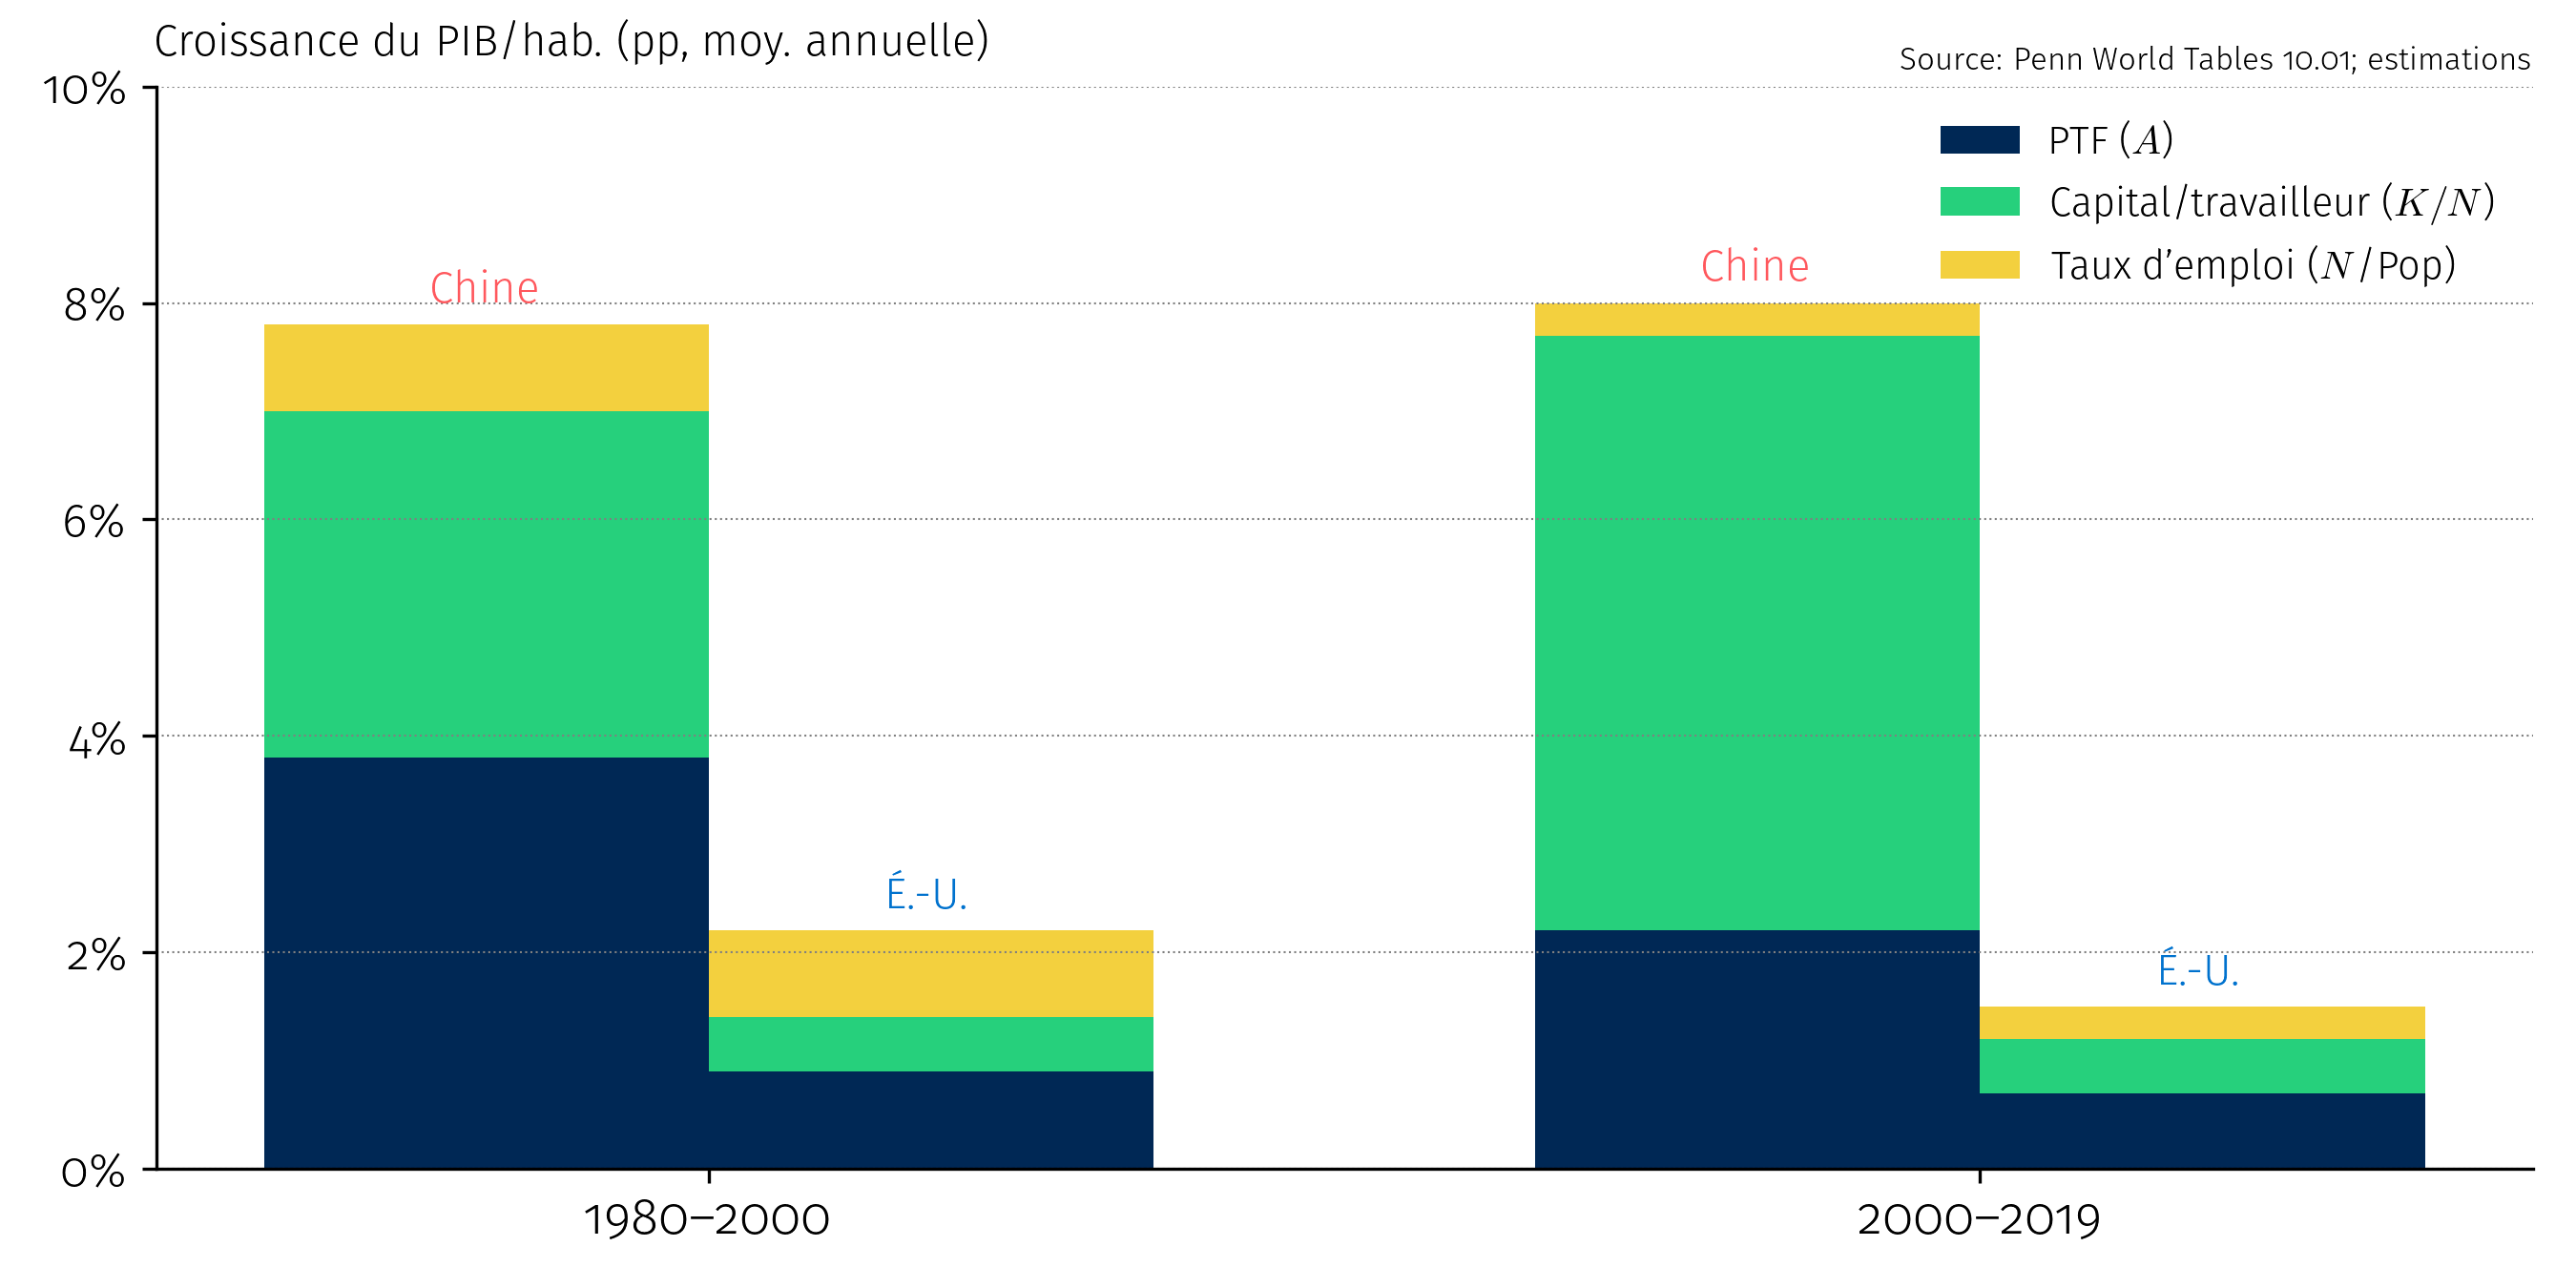
\includegraphics[width=0.95\textwidth]{growth_decomp_china_us.png}
   \end{figure}
\end{frame}

\begin{frame}{Les sources de la croissance mondiale évoluent}
   \begin{figure}
      \centering
      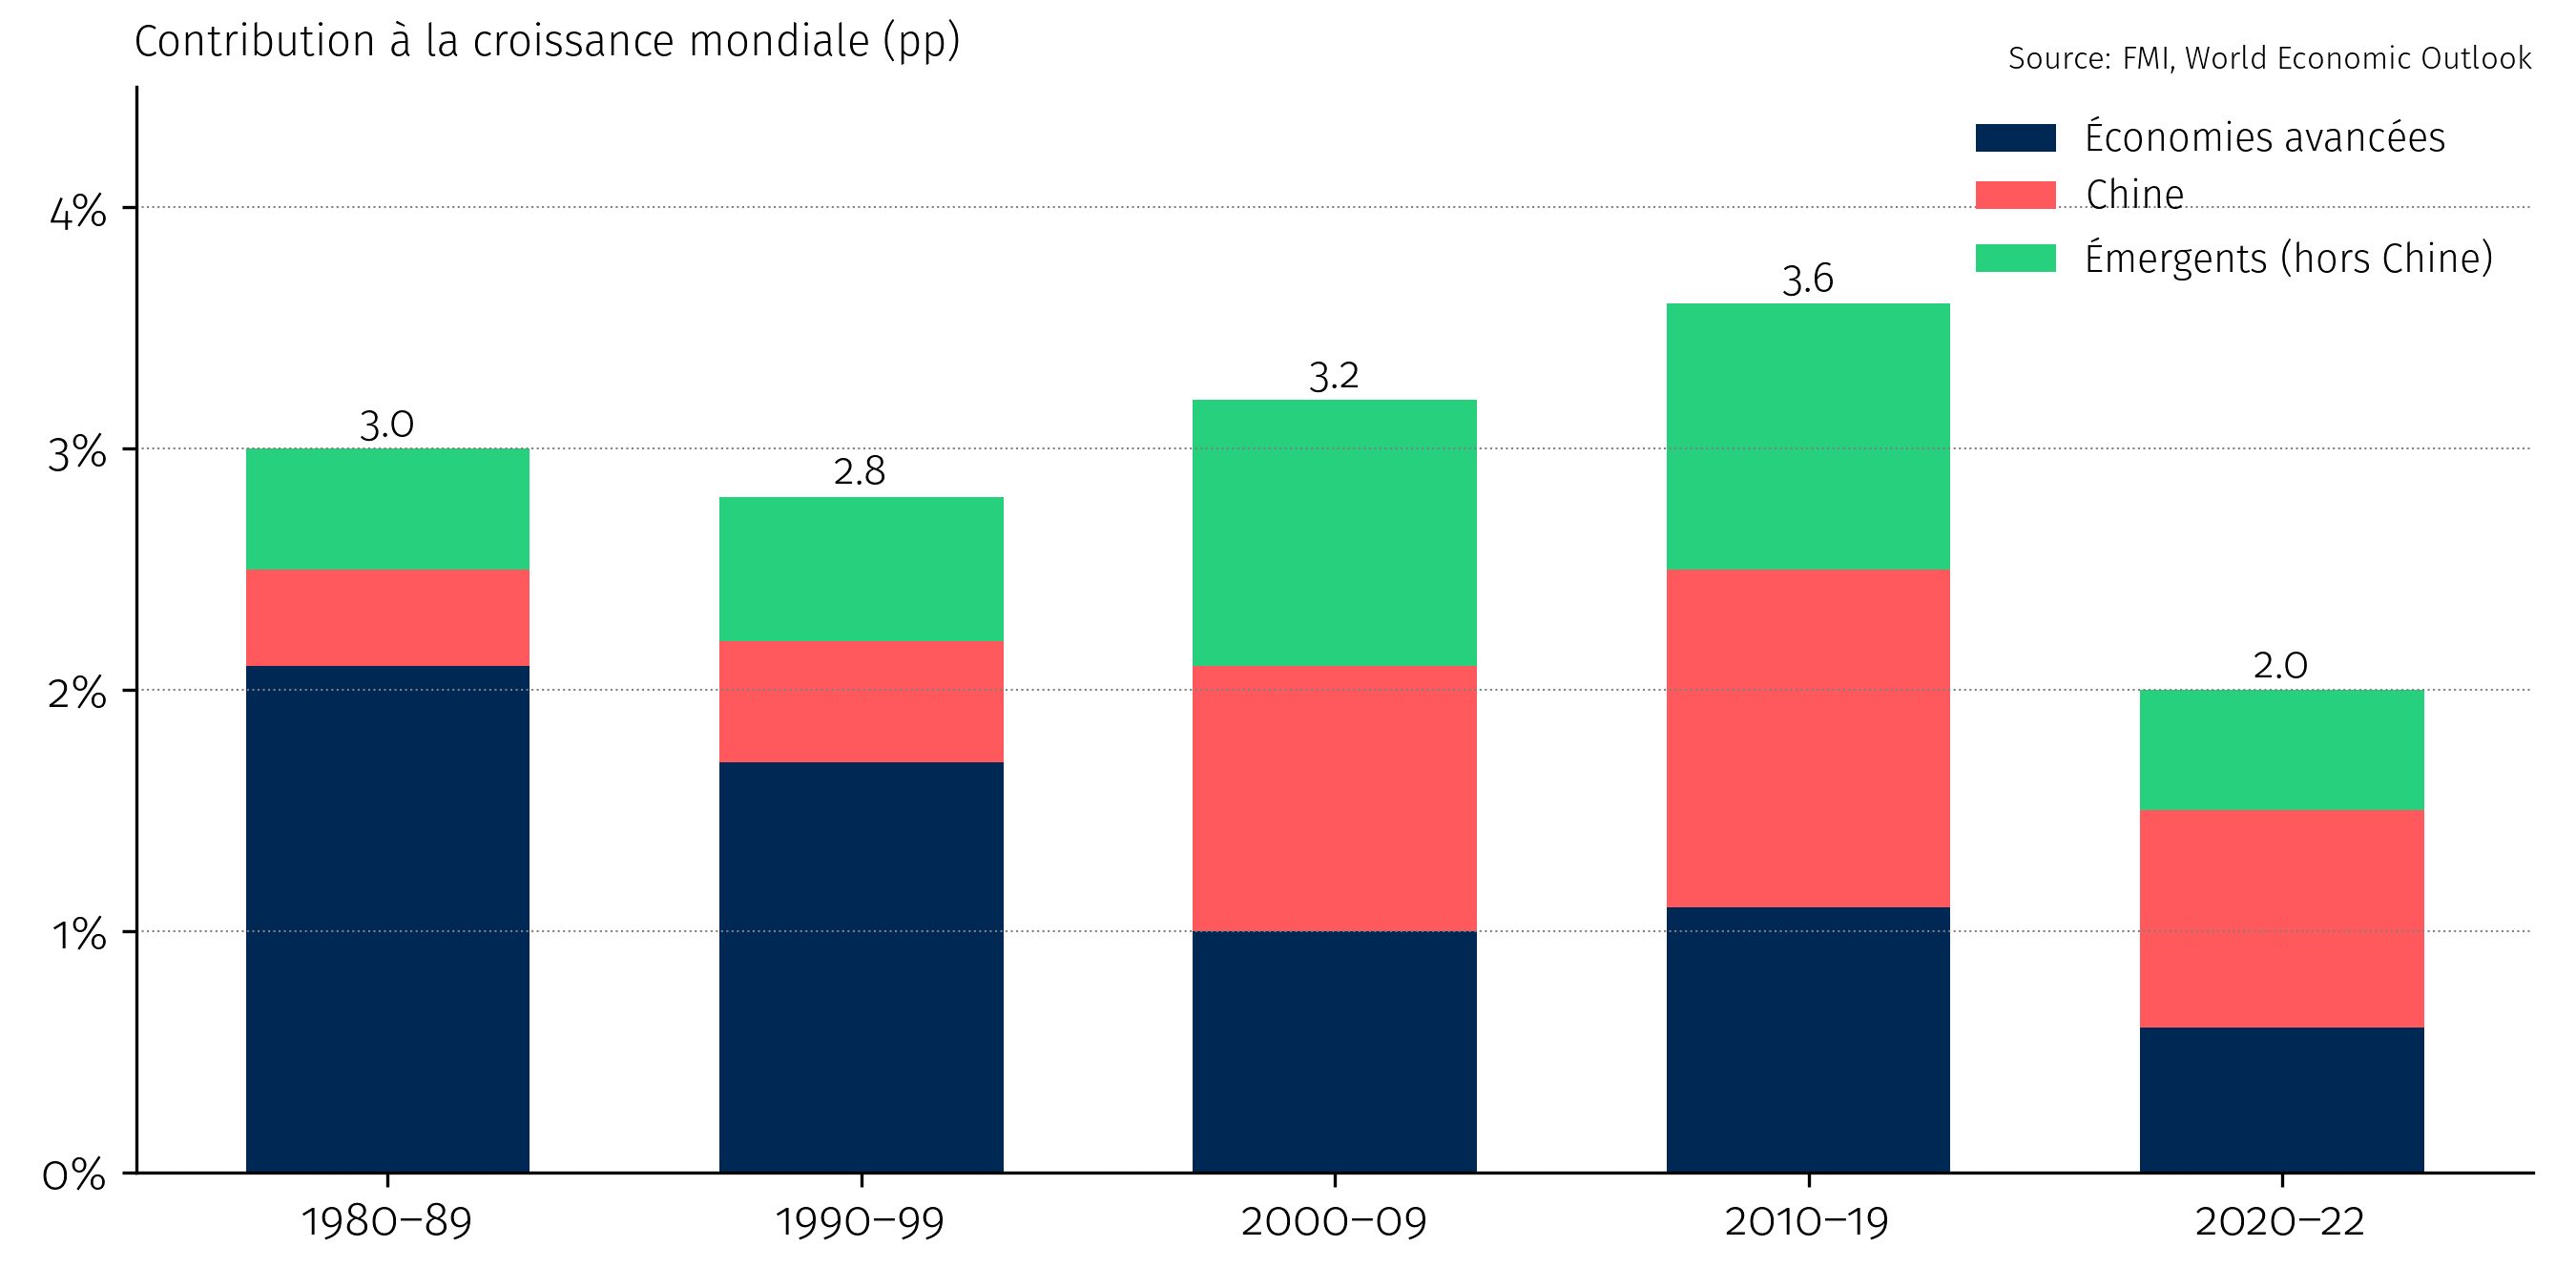
\includegraphics[width=0.95\textwidth]{global_growth_sources.png}
   \end{figure}
\end{frame}

\begin{frame}[t]{La PTF explique $\sim$50\,\% des différences de revenus}
   \vspace{-0.2cm}
   \begin{figure}
      \centering
      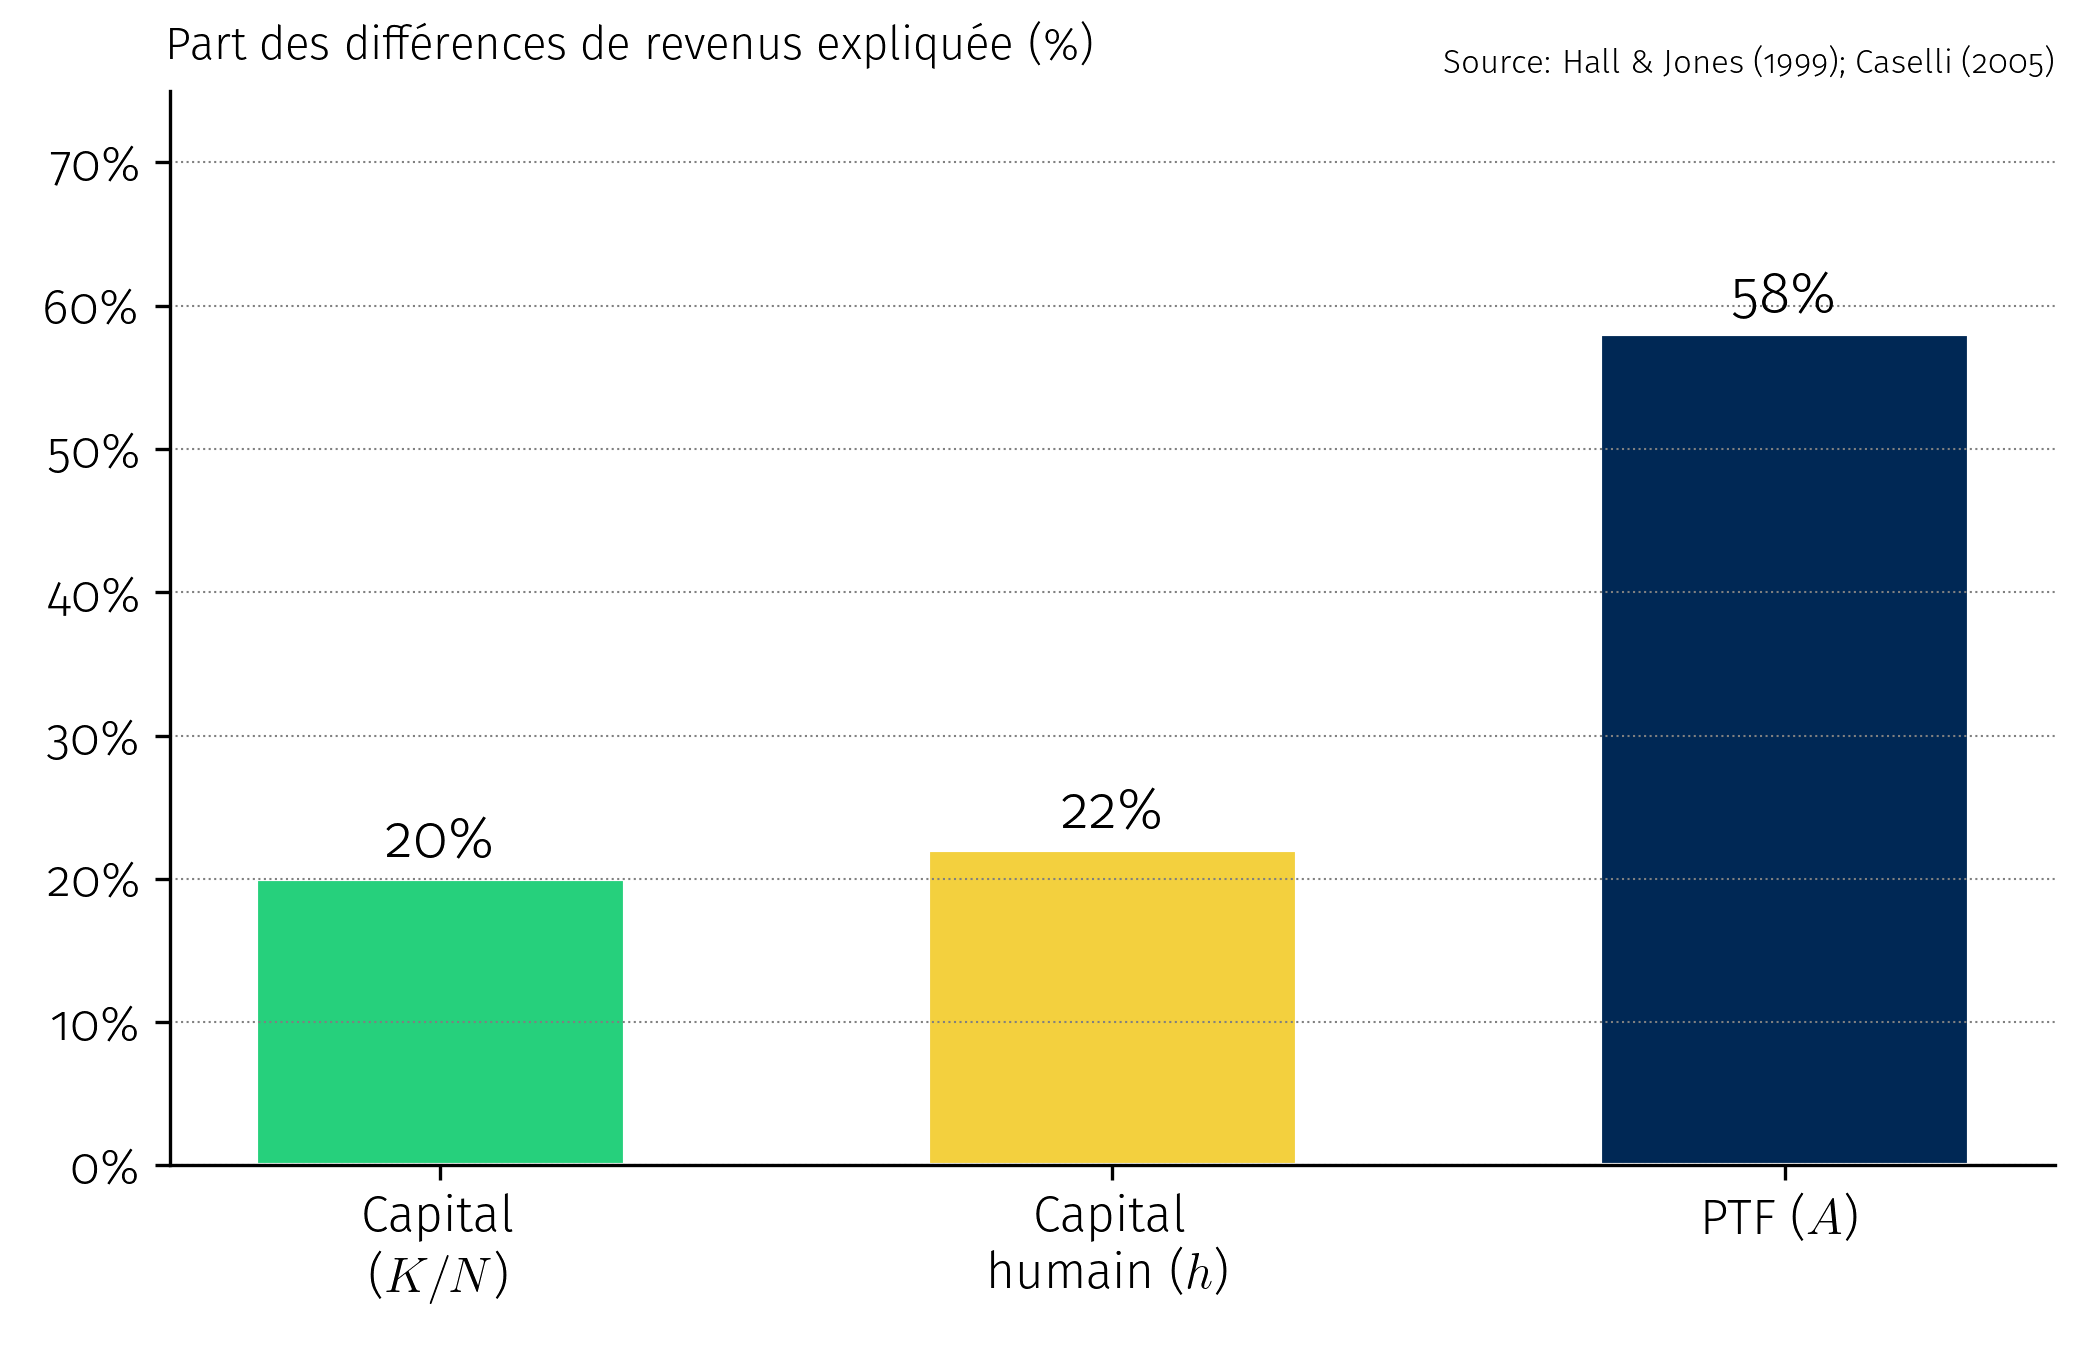
\includegraphics[width=0.85\textwidth, height=0.55\textheight, keepaspectratio]{development_accounting.png}
   \end{figure}
   \vspace{-0.3cm}
   \begin{keyinsight}
      \small Le capital et le travail n'expliquent qu'environ la \textbf{moitié} des différences de revenus entre pays. Le reste : la productivité. Comprendre $A$ est \textbf{la} question centrale.
   \end{keyinsight}
\end{frame}

\begin{frame}{Qu'est-ce qui détermine $K/N$?}
   On peut \textit{mesurer} les sources de la croissance. Mais qu'est-ce qui \textbf{détermine} l'accumulation de capital?
   \vspace{0.3cm}
   \begin{itemize}
      \setlength\itemsep{0.2cm}
      \item Pourquoi certains pays investissent-ils plus que d'autres?
      \item L'investissement massif peut-il à lui seul assurer la croissance?
      \item Y a-t-il des \textbf{limites} à l'accumulation de capital?
   \end{itemize}
   \vspace{0.3cm}
   Pour répondre, nous avons besoin d'un modèle qui décrit la \textbf{dynamique} du capital $\to$ le \textbf{modèle de Solow}
\end{frame}

% ============================================================================
\begin{frame}{Plan}
   \begin{enumerate}
      \setlength\itemsep{0.25cm}
      \item {\color{gray!50}La croissance est un phénomène récent}
      \item {\color{gray!50}La fonction de production}
      \item {\color{gray!50}Décomposer la croissance}
      \item \textbf{Le modèle de Solow}
      \item Convergence
      \item Le vrai moteur de la croissance
      \item Le casse-tête canadien de la productivité
      \item Croissance et environnement
   \end{enumerate}
\end{frame}

% ============================================================================
\sectionframe{Le modèle de Solow}
% ============================================================================

\begin{frame}[t]{Robert Solow (1924--2023)}
   \begin{columns}[T]
      \begin{column}{0.6\textwidth}
         \begin{itemize}
            \setlength\itemsep{0.15cm}
            \item Admis à Harvard à 16 ans
            \item Service militaire en Italie pendant la Seconde Guerre mondiale
            \item Professeur au MIT pendant plus de 50 ans
            \item \textbf{Prix Nobel d'économie} en 1987
            \item Son modèle (1956) reste \textit{le} cadre de référence pour analyser la croissance de long terme
         \end{itemize}
         \vspace{0.15cm}
         {\small\textcolor{HECgray}{\guillemotleft~Everything reminds Milton [Friedman] of the money supply. Well, everything reminds me of sex, but I keep it out of the paper.~\guillemotright}}
      \end{column}
      \begin{column}{0.35\textwidth}
         \centering
         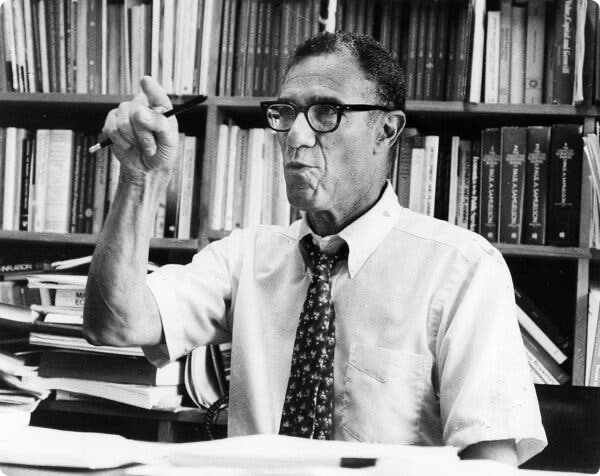
\includegraphics[width=\textwidth, keepaspectratio]{solow.png}
      \end{column}
   \end{columns}
\end{frame}

\begin{frame}[t]{L'expérience de guerre de Solow}
   \begin{columns}[T]
      \begin{column}{0.48\textwidth}
         \centering
         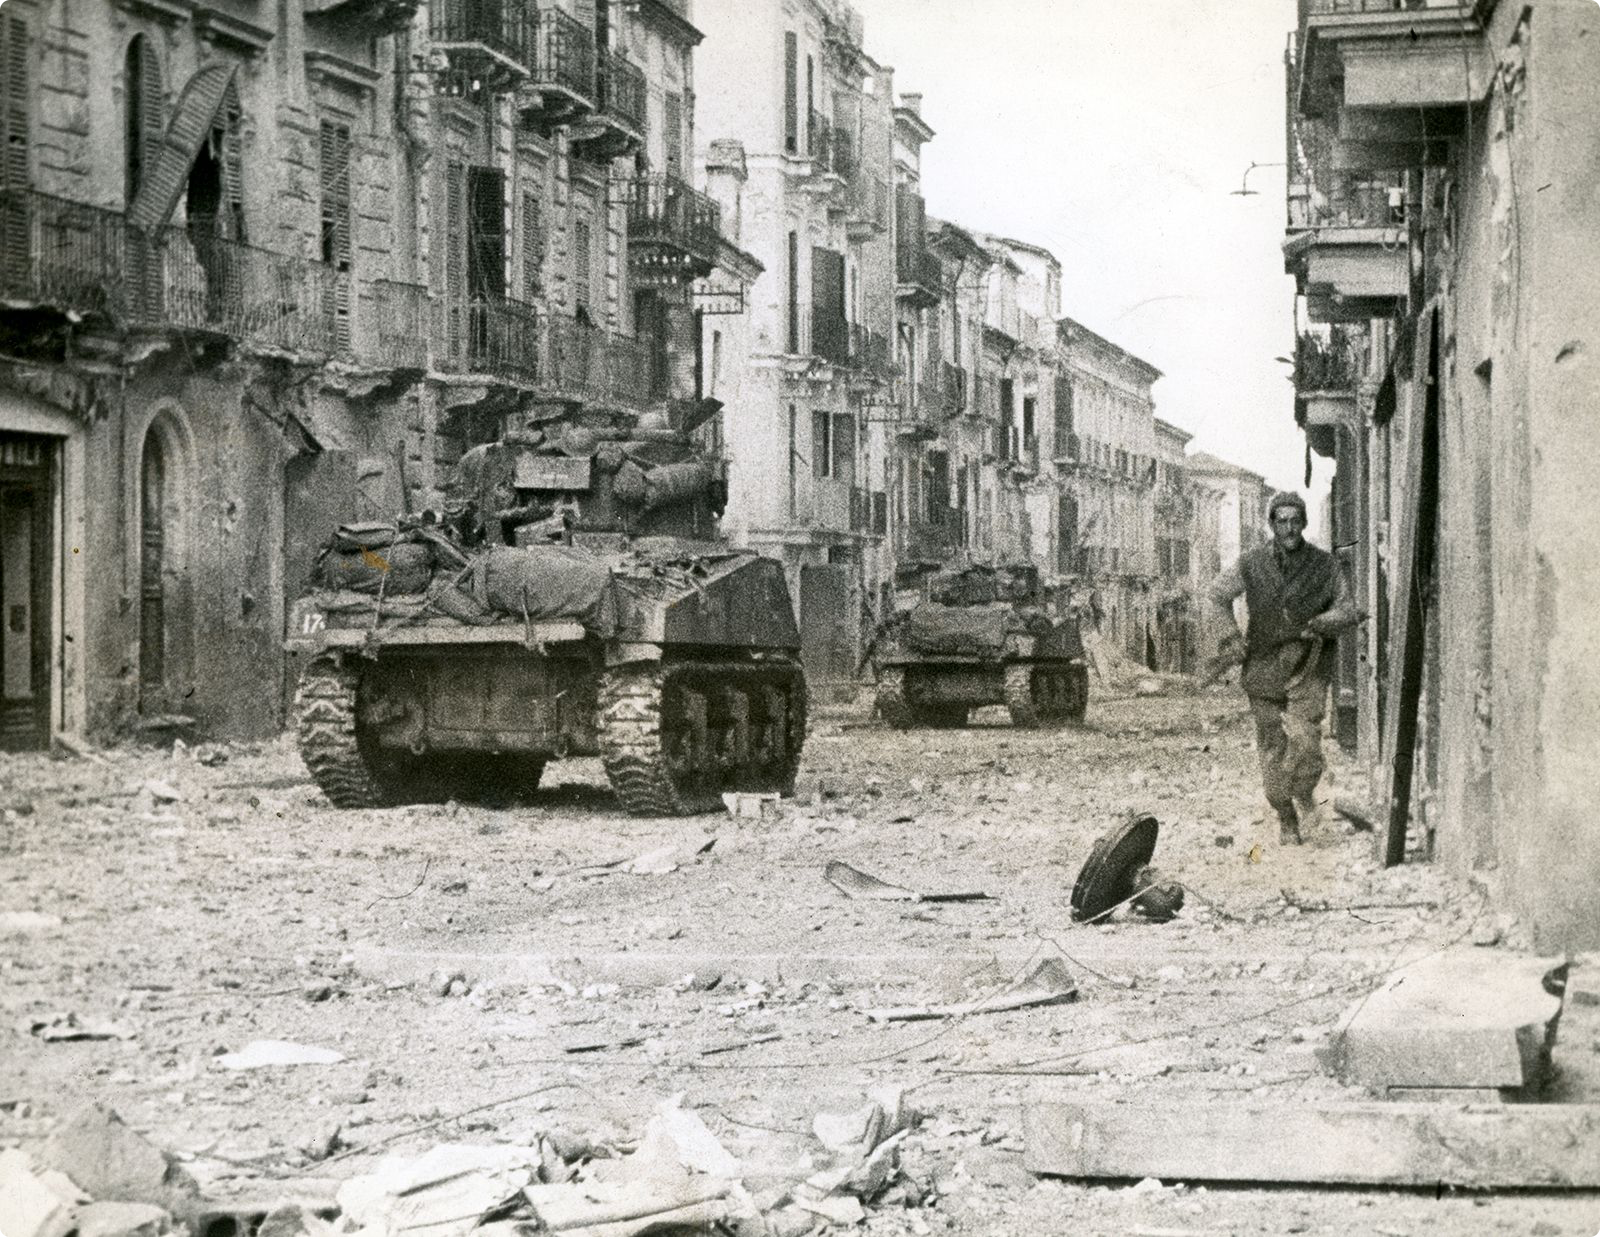
\includegraphics[width=\textwidth, height=0.65\textheight, keepaspectratio]{italy_1.png}
      \end{column}
      \begin{column}{0.48\textwidth}
         \centering
         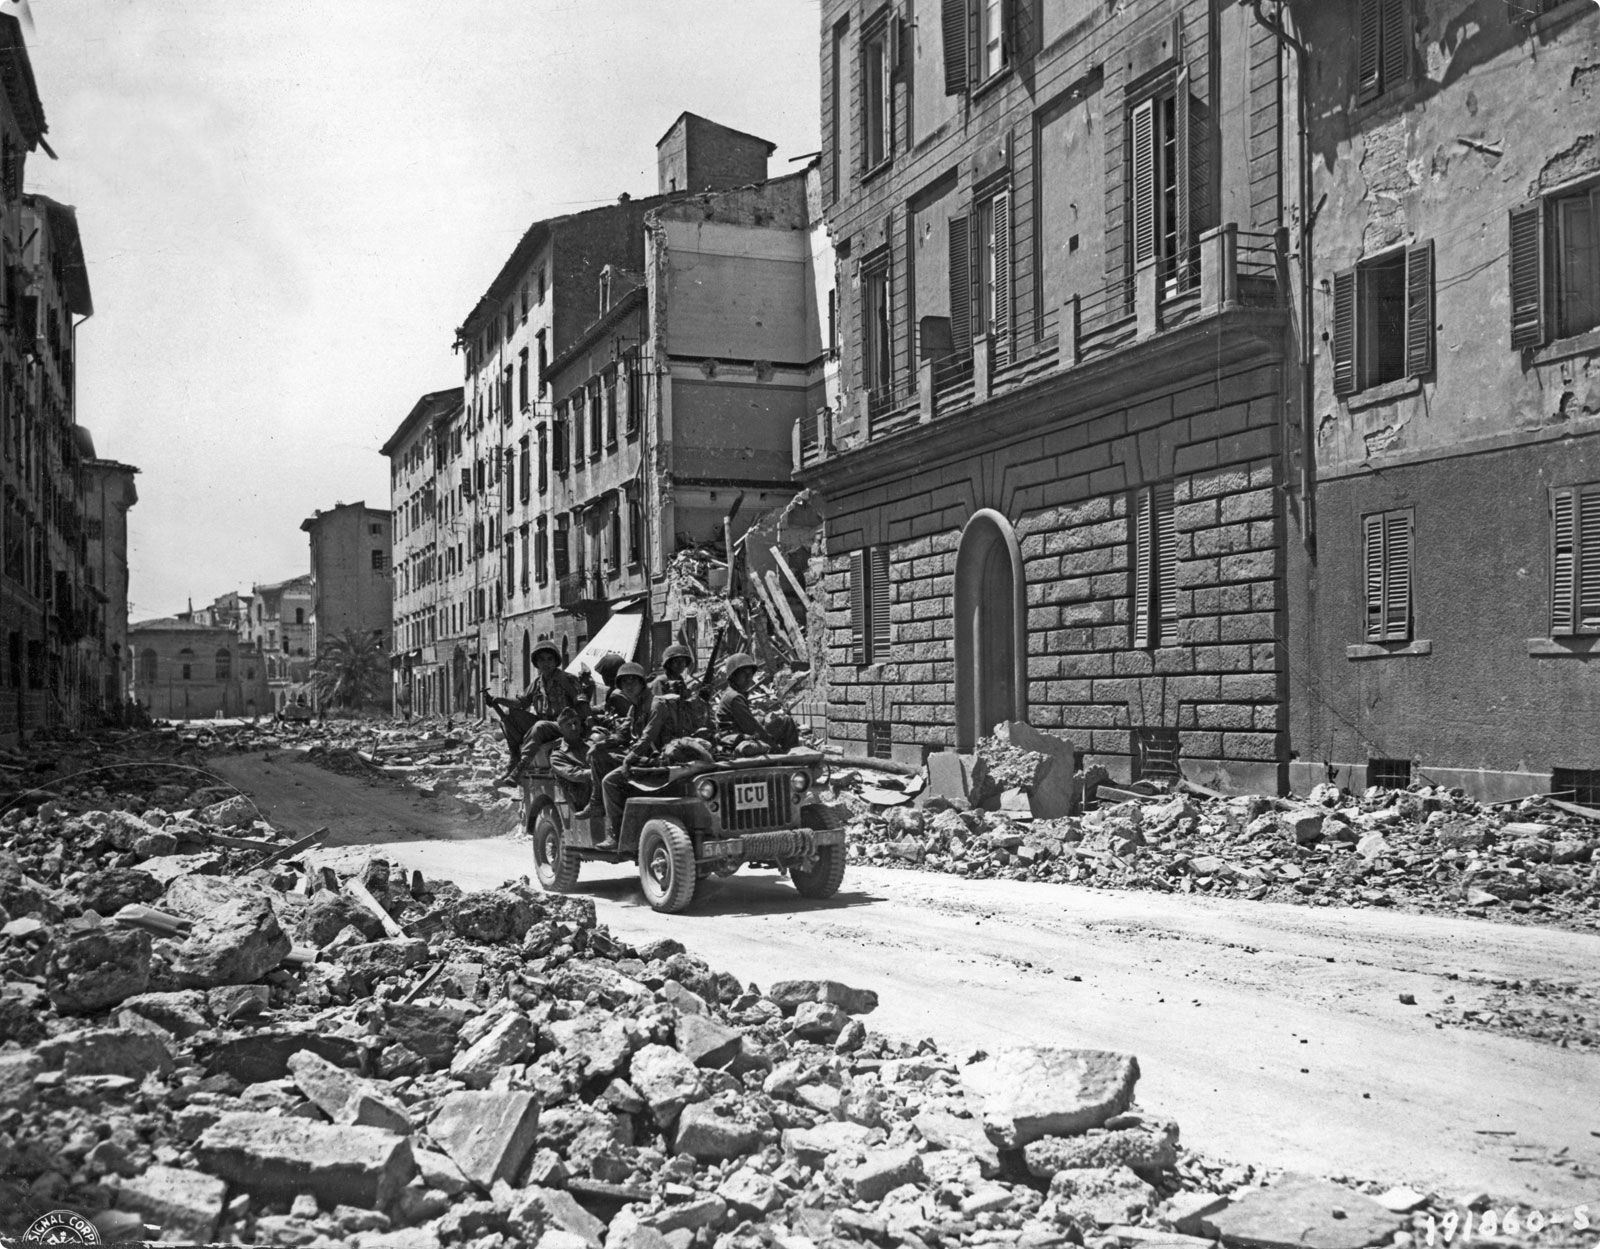
\includegraphics[width=\textwidth, height=0.65\textheight, keepaspectratio]{italy_2.png}
      \end{column}
   \end{columns}
   \vspace{0.2cm}
   \centering
   {\small Le capital a été \textbf{massivement détruit}\ldots mais les pays se sont \textbf{entièrement remis}.\\Qu'est-ce qui détermine la reprise?}
\end{frame}

\begin{frame}{La reprise d'après-guerre}
   \begin{figure}
      \centering
      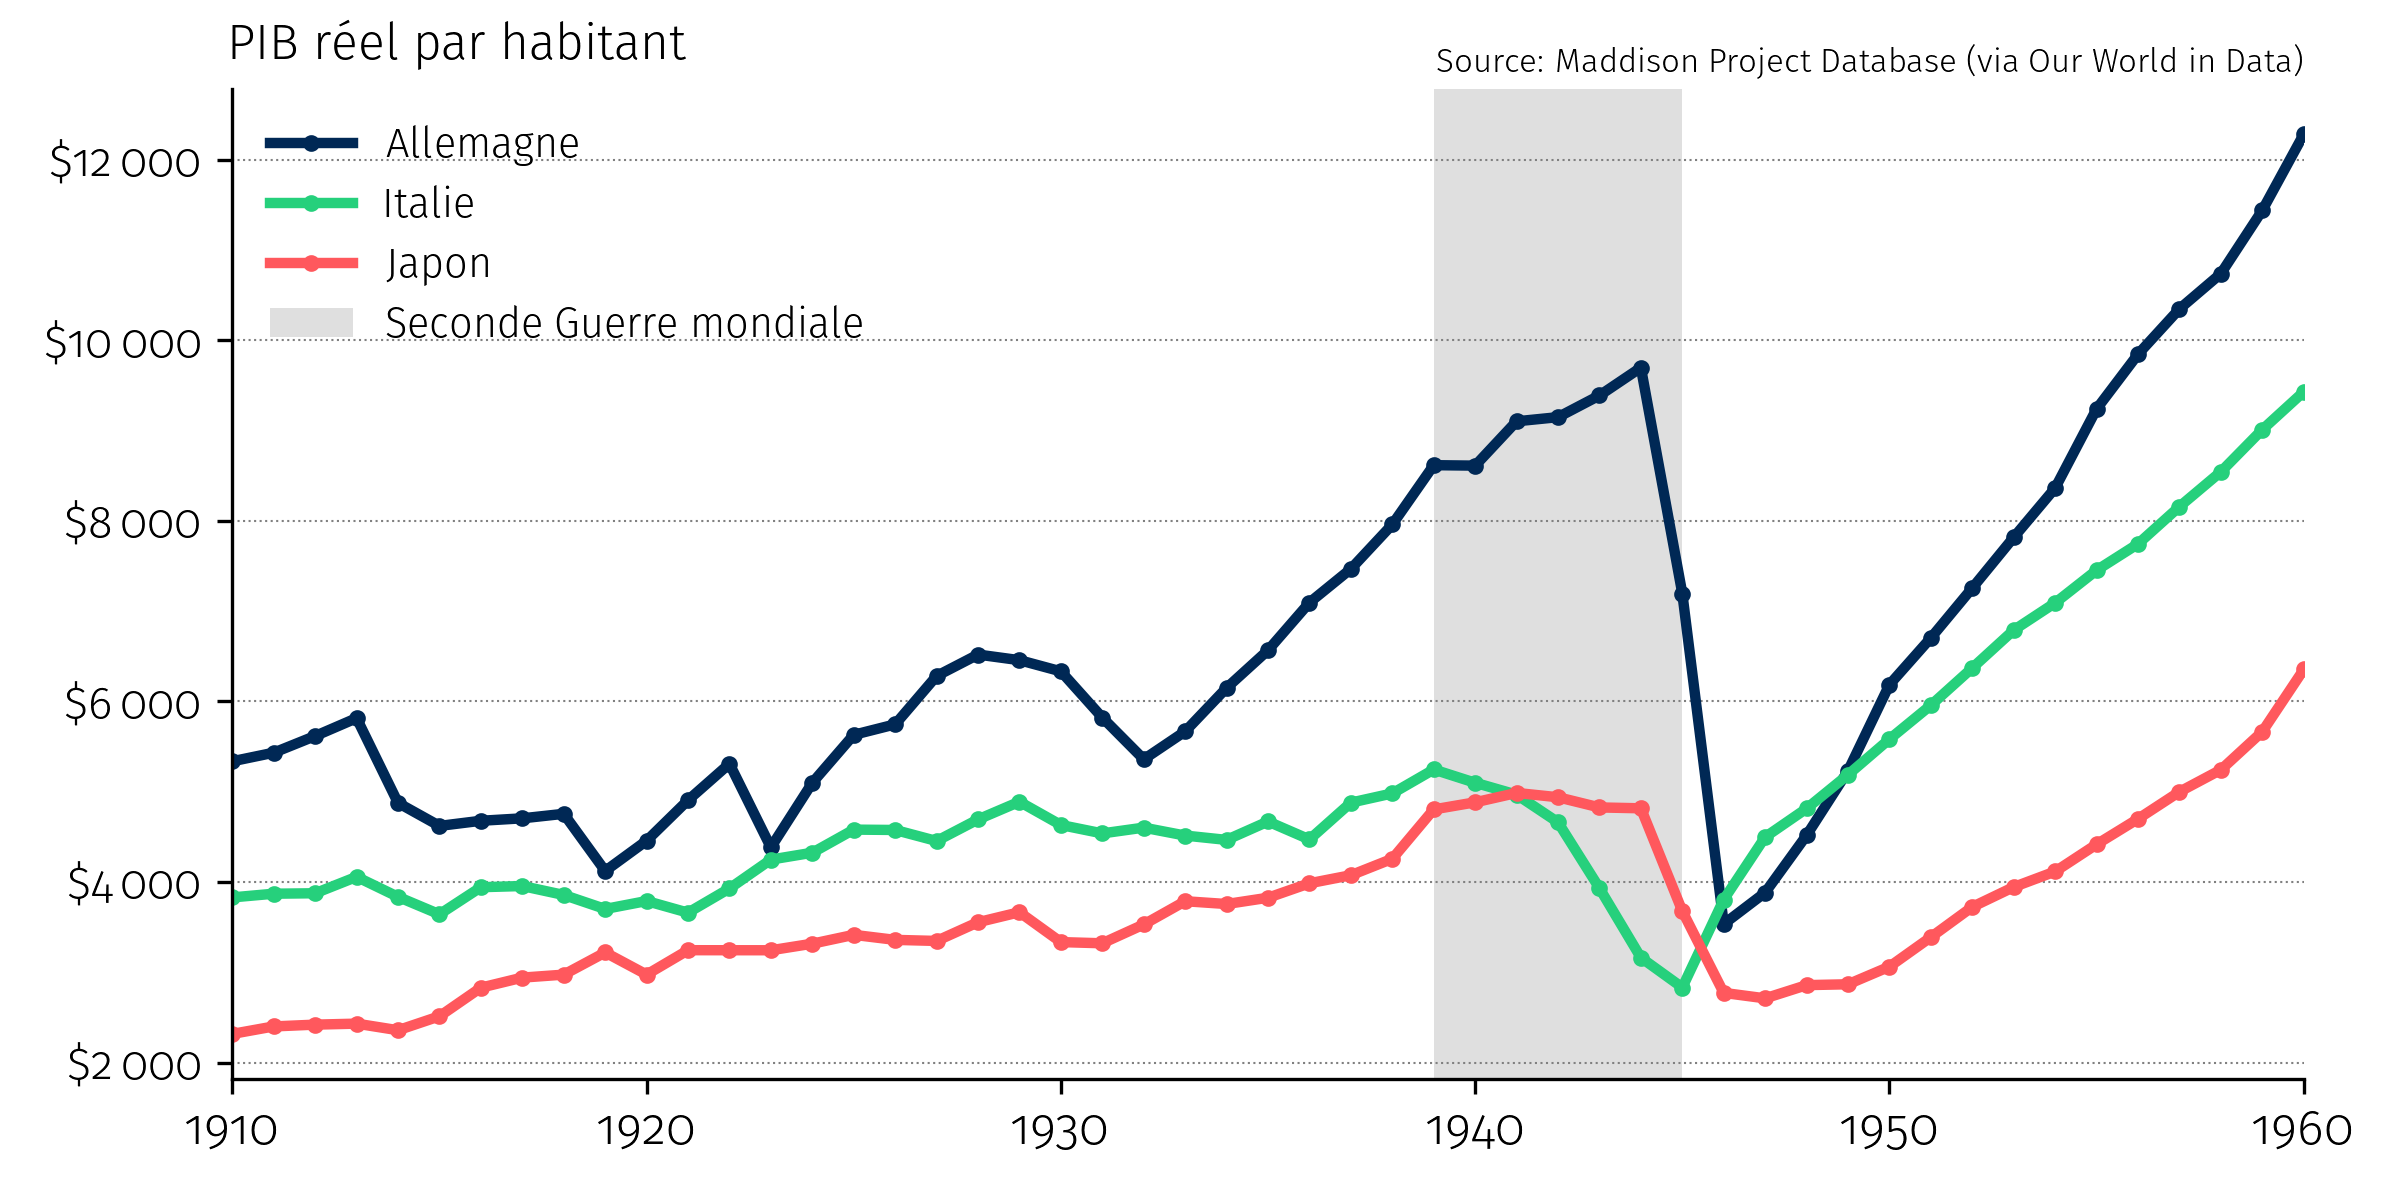
\includegraphics[width=0.9\textwidth]{ww2_recovery.png}
   \end{figure}
\end{frame}

\begin{frame}[t]{Les conclusions surprenantes de Solow}
   \vspace{0.3cm}
   \begin{enumerate}
      \setlength\itemsep{0.4cm}
      \item Le capital est \textbf{crucial} pour le niveau de vie\ldots
      \item \ldots mais l'accumulation de capital \textbf{seule} ne peut pas soutenir la croissance à long terme!
   \end{enumerate}
   \vspace{0.3cm}
   \begin{warning}
      Investir massivement vous rend plus \textbf{riche}, mais ne vous fait pas croître plus \textbf{vite} indéfiniment. Les rendements décroissants finissent toujours par dominer.
   \end{warning}
\end{frame}

\begin{frame}[t]{L'analogie de la baignoire}
   \small
   Imaginez le stock de capital par travailleur ($K/N$) comme le niveau d'eau dans une baignoire :
   \vspace{0.2cm}
   \begin{columns}[T]
      \begin{column}{0.48\textwidth}
         \textbf{\textcolor{HECnavy}{Le robinet (entrée)}}
         \vspace{0.1cm}
         \begin{itemize}
            \setlength\itemsep{0.1cm}
            \item Investissement = $s \cdot Y$
            \item $s$ = taux d'épargne/investissement
            \item Plus la baignoire est vide, plus le débit est \guillemotleft~utile~\guillemotright
         \end{itemize}
      \end{column}
      \begin{column}{0.48\textwidth}
         \textbf{\textcolor{HECcoral}{Le drain (sortie)}}
         \vspace{0.1cm}
         \begin{itemize}
            \setlength\itemsep{0.1cm}
            \item Dépréciation = $\delta \cdot K$
            \item Croissance de la population = $n$
            \item Plus le niveau est élevé, plus le drain est fort
         \end{itemize}
      \end{column}
   \end{columns}
   \vspace{0.2cm}
   \begin{defbox}[Équilibre de long terme]
      Quand entrée $=$ sortie, le niveau se stabilise. C'est l'\textbf{état stationnaire} : $K/N$ ne change plus.
   \end{defbox}
\end{frame}

\begin{frame}[t]{La baignoire : exercice}
   \small
   \begin{exercise}
      Une baignoire a une capacité de 100 litres. Le robinet coule à 5\,L/min. Le drain évacue 10\,\% du contenu par minute.
      \vspace{0.15cm}
      \begin{enumerate}
         \setlength\itemsep{0.15cm}
         \item Si le niveau initial est de \textbf{10 litres}, que se passe-t-il? (drain = 1\,L/min $<$ 5\,L/min $\to$ le niveau \textbf{monte})
         \item Si le niveau initial est de \textbf{90 litres}? (drain = 9\,L/min $>$ 5\,L/min $\to$ le niveau \textbf{baisse})
         \item Quel est le \textbf{niveau d'équilibre}? (quand drain = robinet : $0{,}10 \times K = 5 \to K = 50$)
         \item Le niveau initial \textbf{affecte-t-il} l'équilibre de long terme?
      \end{enumerate}
   \end{exercise}
\end{frame}

\begin{frame}[t]{Les enseignements de Solow}
   \small
   \begin{enumerate}
      \setlength\itemsep{0.25cm}
      \item \textbf{Le point de départ n'a pas d'importance à long terme}\\
      {\small Peu importe que $K/N$ soit faible ou élevé --- l'économie converge vers le même état stationnaire}
      \item \textbf{Plus d'investissement $\to$ plus riche, mais PAS une croissance plus rapide}\\
      {\small Un taux d'épargne plus élevé ($s \uparrow$) élève le niveau de $K/N$, mais la croissance s'arrête au nouvel état stationnaire}
      \item \textbf{Plus de croissance démographique $\to$ moins riche}\\
      {\small Le capital doit être réparti entre plus de travailleurs ($n \uparrow \to K/N \downarrow$)}
   \end{enumerate}
   \vspace{0.15cm}
   \begin{keyinsight}
      Tous ces résultats sont des résultats \textit{ceteris paribus} et de \textit{long terme}.
   \end{keyinsight}
\end{frame}

\begin{frame}[t]{Application : la Chine ralentit}
   \vspace{-0.2cm}
   \begin{figure}
      \centering
      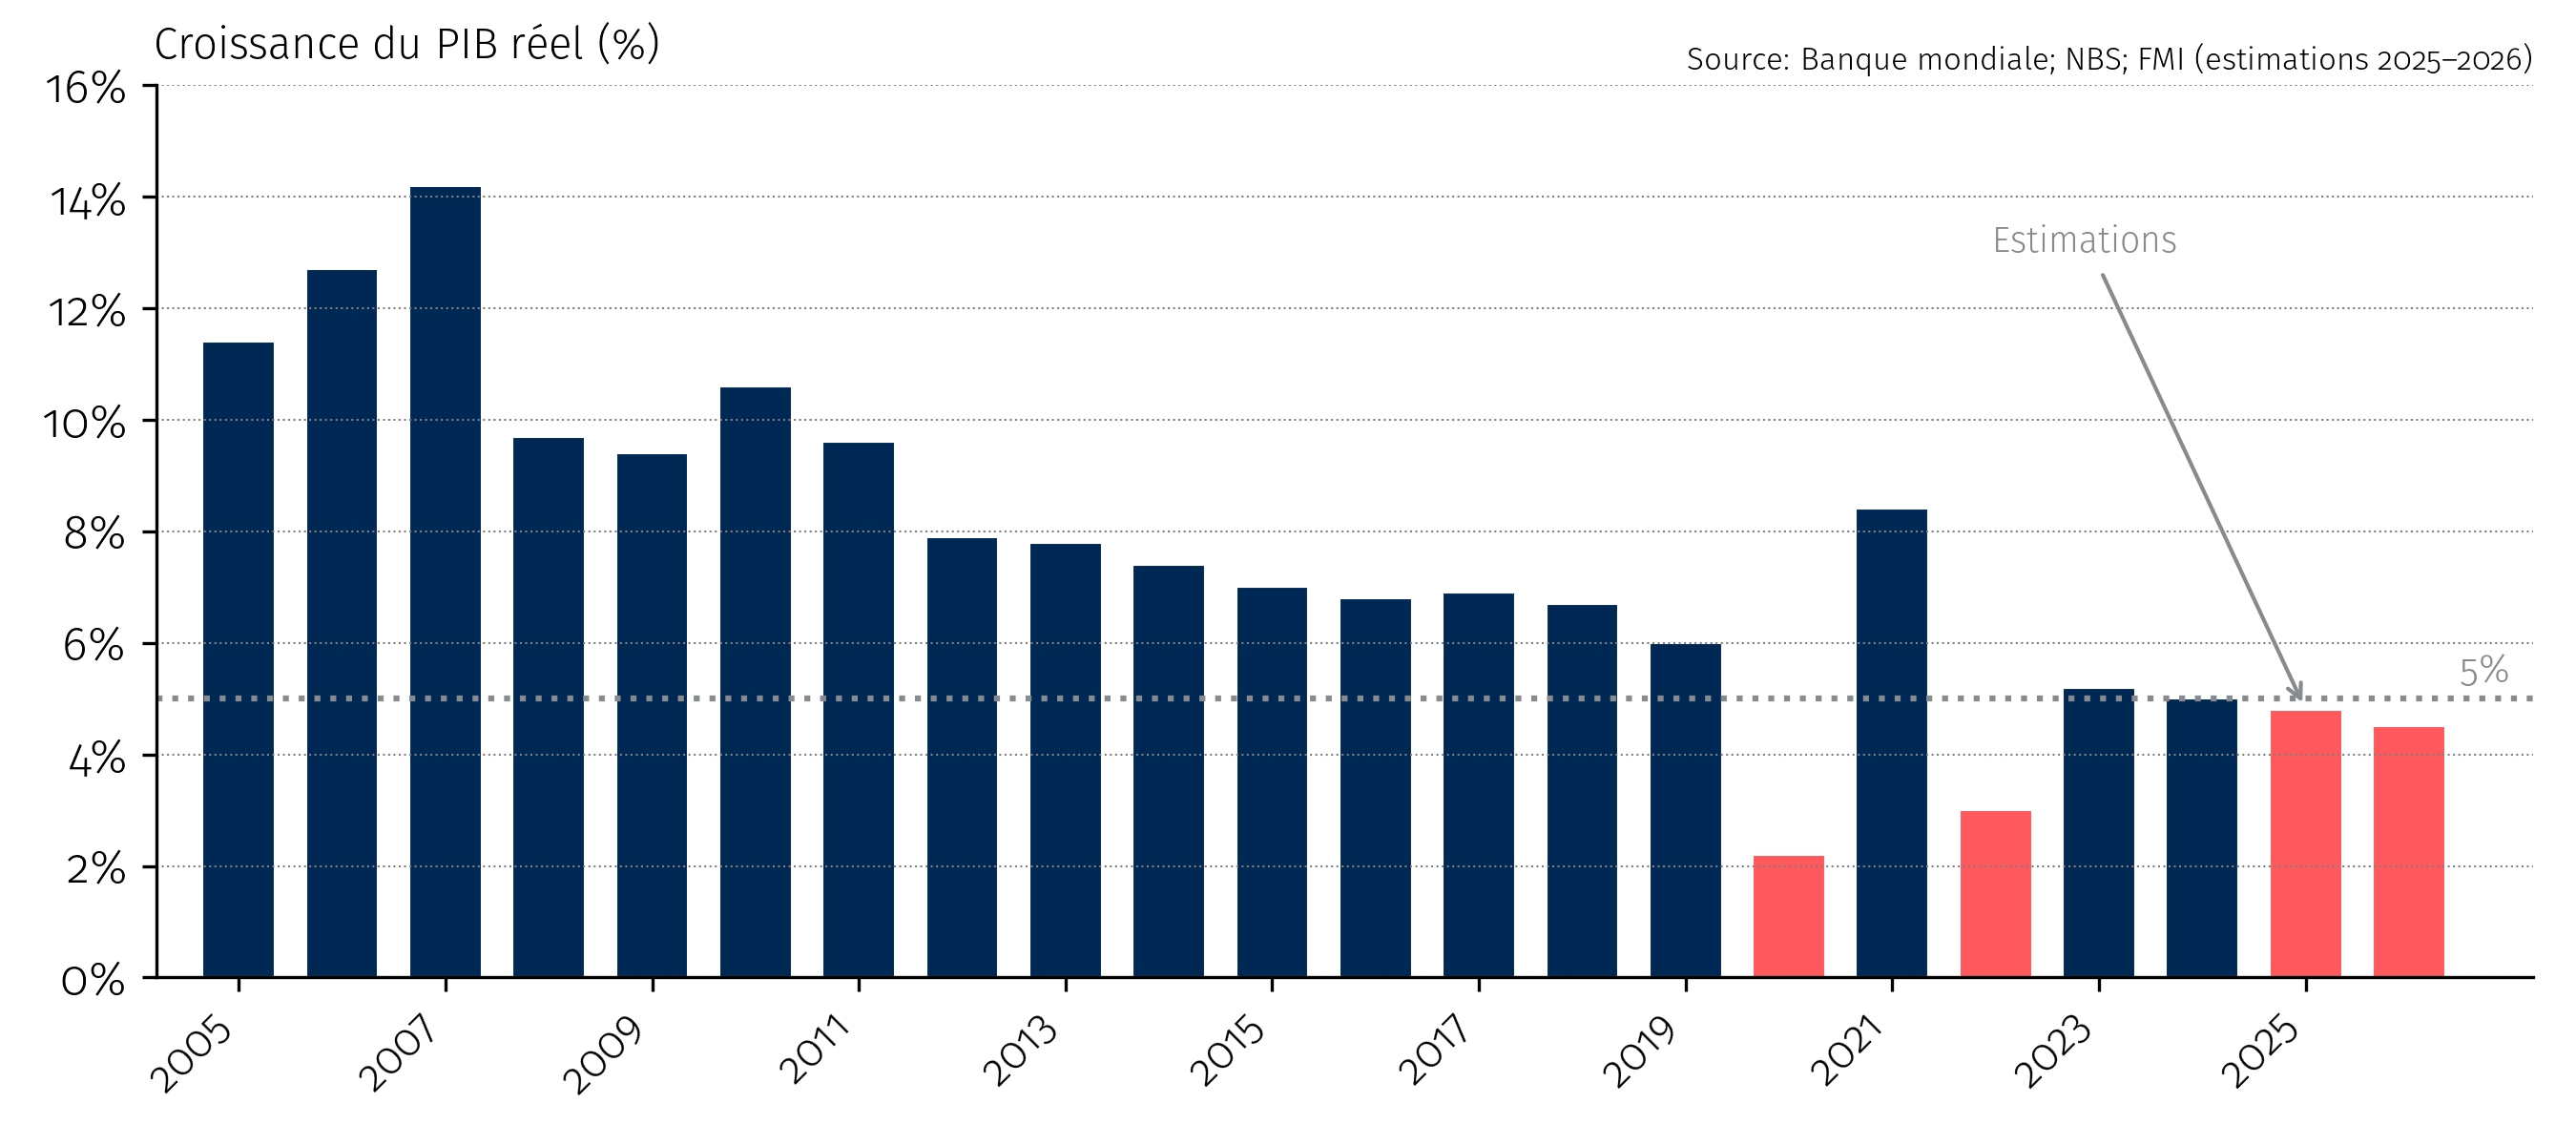
\includegraphics[width=0.85\textwidth, height=0.55\textheight, keepaspectratio]{china_gdp_growth.png}
   \end{figure}
   \vspace{-0.3cm}
   \begin{bizimplication}
      \footnotesize La croissance chinoise a été tirée par l'accumulation massive de capital. Solow prédit que cette stratégie atteint ses limites --- les rendements décroissants finissent par dominer.
   \end{bizimplication}
\end{frame}

\begin{frame}[t]{Application : une croissance sur la dette}
   % TODO: Replace with actual chart of China fiscal deficit (official vs augmented)
   \begin{tcolorbox}[
      colback=HEClightgray, colframe=HEClightgray, arc=8pt,
      width=\textwidth, height=0.45\textheight,
      halign=center, valign=center
   ]
      {\large\itshape\textcolor{HECgray}{Graphique : déficit fiscal chinois (officiel vs.\ augmenté)}}\\[6pt]
      {\small\textcolor{HECgray}{Source : IMF, Rhodium Group}}
   \end{tcolorbox}
   \vspace{0.05cm}
   \begin{warning}
      \footnotesize La Chine a financé son accumulation de capital par un endettement massif. \guillemotleft~850 milliards de nouvelle dette en un trimestre.~\guillemotright\ Quand l'investissement est alimenté par la dette plutôt que l'épargne, les risques s'accumulent.
   \end{warning}
\end{frame}

\begin{frame}[t]{Application : la destruction de capital}
   \small
   La Seconde Guerre mondiale a détruit une part massive du stock de capital en Europe et au Japon.
   \vspace{0.15cm}

   Pourtant, ces économies ont retrouvé leur trajectoire de croissance en 15--20 ans.
   \vspace{0.15cm}

   \textbf{Pourquoi?} Solow a la réponse :
   \vspace{0.1cm}
   \begin{itemize}
      \setlength\itemsep{0.08cm}
      \item La destruction de capital éloigne l'économie de son état stationnaire
      \item Mais les \textbf{paramètres fondamentaux} ($s$, $n$, $\delta$, $A$) n'ont pas changé
      \item Le mécanisme de la baignoire ramène l'économie à l'équilibre
   \end{itemize}
   \vspace{0.1cm}
   \begin{defbox}[Implication clé]
      L'équilibre de long terme dépend des \textbf{paramètres} ($s$, $n$, $\delta$, $A$), pas du point de départ.
   \end{defbox}
\end{frame}

% ============================================================================
\begin{frame}{Plan}
   \begin{enumerate}
      \setlength\itemsep{0.25cm}
      \item {\color{gray!50}La croissance est un phénomène récent}
      \item {\color{gray!50}La fonction de production}
      \item {\color{gray!50}Décomposer la croissance}
      \item {\color{gray!50}Le modèle de Solow}
      \item \textbf{Convergence}
      \item Le vrai moteur de la croissance
      \item Le casse-tête canadien de la productivité
      \item Croissance et environnement
   \end{enumerate}
\end{frame}

% ============================================================================
\sectionframe{Convergence}
% ============================================================================

\begin{frame}[t]{Les pays pauvres rattrapent-ils les pays riches?}
   \textbf{Prédiction de Solow :} les pays pauvres devraient croître \textbf{plus vite}
   \vspace{0.2cm}
   \begin{itemize}
      \setlength\itemsep{0.15cm}
      \item Pays pauvre $\to$ faible $K/N$ $\to$ rendement marginal du capital \textbf{élevé}
      \item Chaque dollar investi génère plus de production
      \item L'écart entre le robinet et le drain est \textbf{maximal}
   \end{itemize}
   \vspace{0.2cm}
   \begin{itemize}
      \setlength\itemsep{0.15cm}
      \item Pays riche $\to$ élevé $K/N$ $\to$ rendement marginal \textbf{faible}
      \item Le drain est presque aussi fort que le robinet
      \item La croissance ralentit naturellement
   \end{itemize}
   \vspace{0.2cm}
   $\to$ Les pays pauvres devraient \textbf{converger} vers les pays riches. Est-ce le cas?
\end{frame}

\begin{frame}{Convergence entre États américains}
   \vspace{-0.2cm}
   \begin{figure}
      \centering
      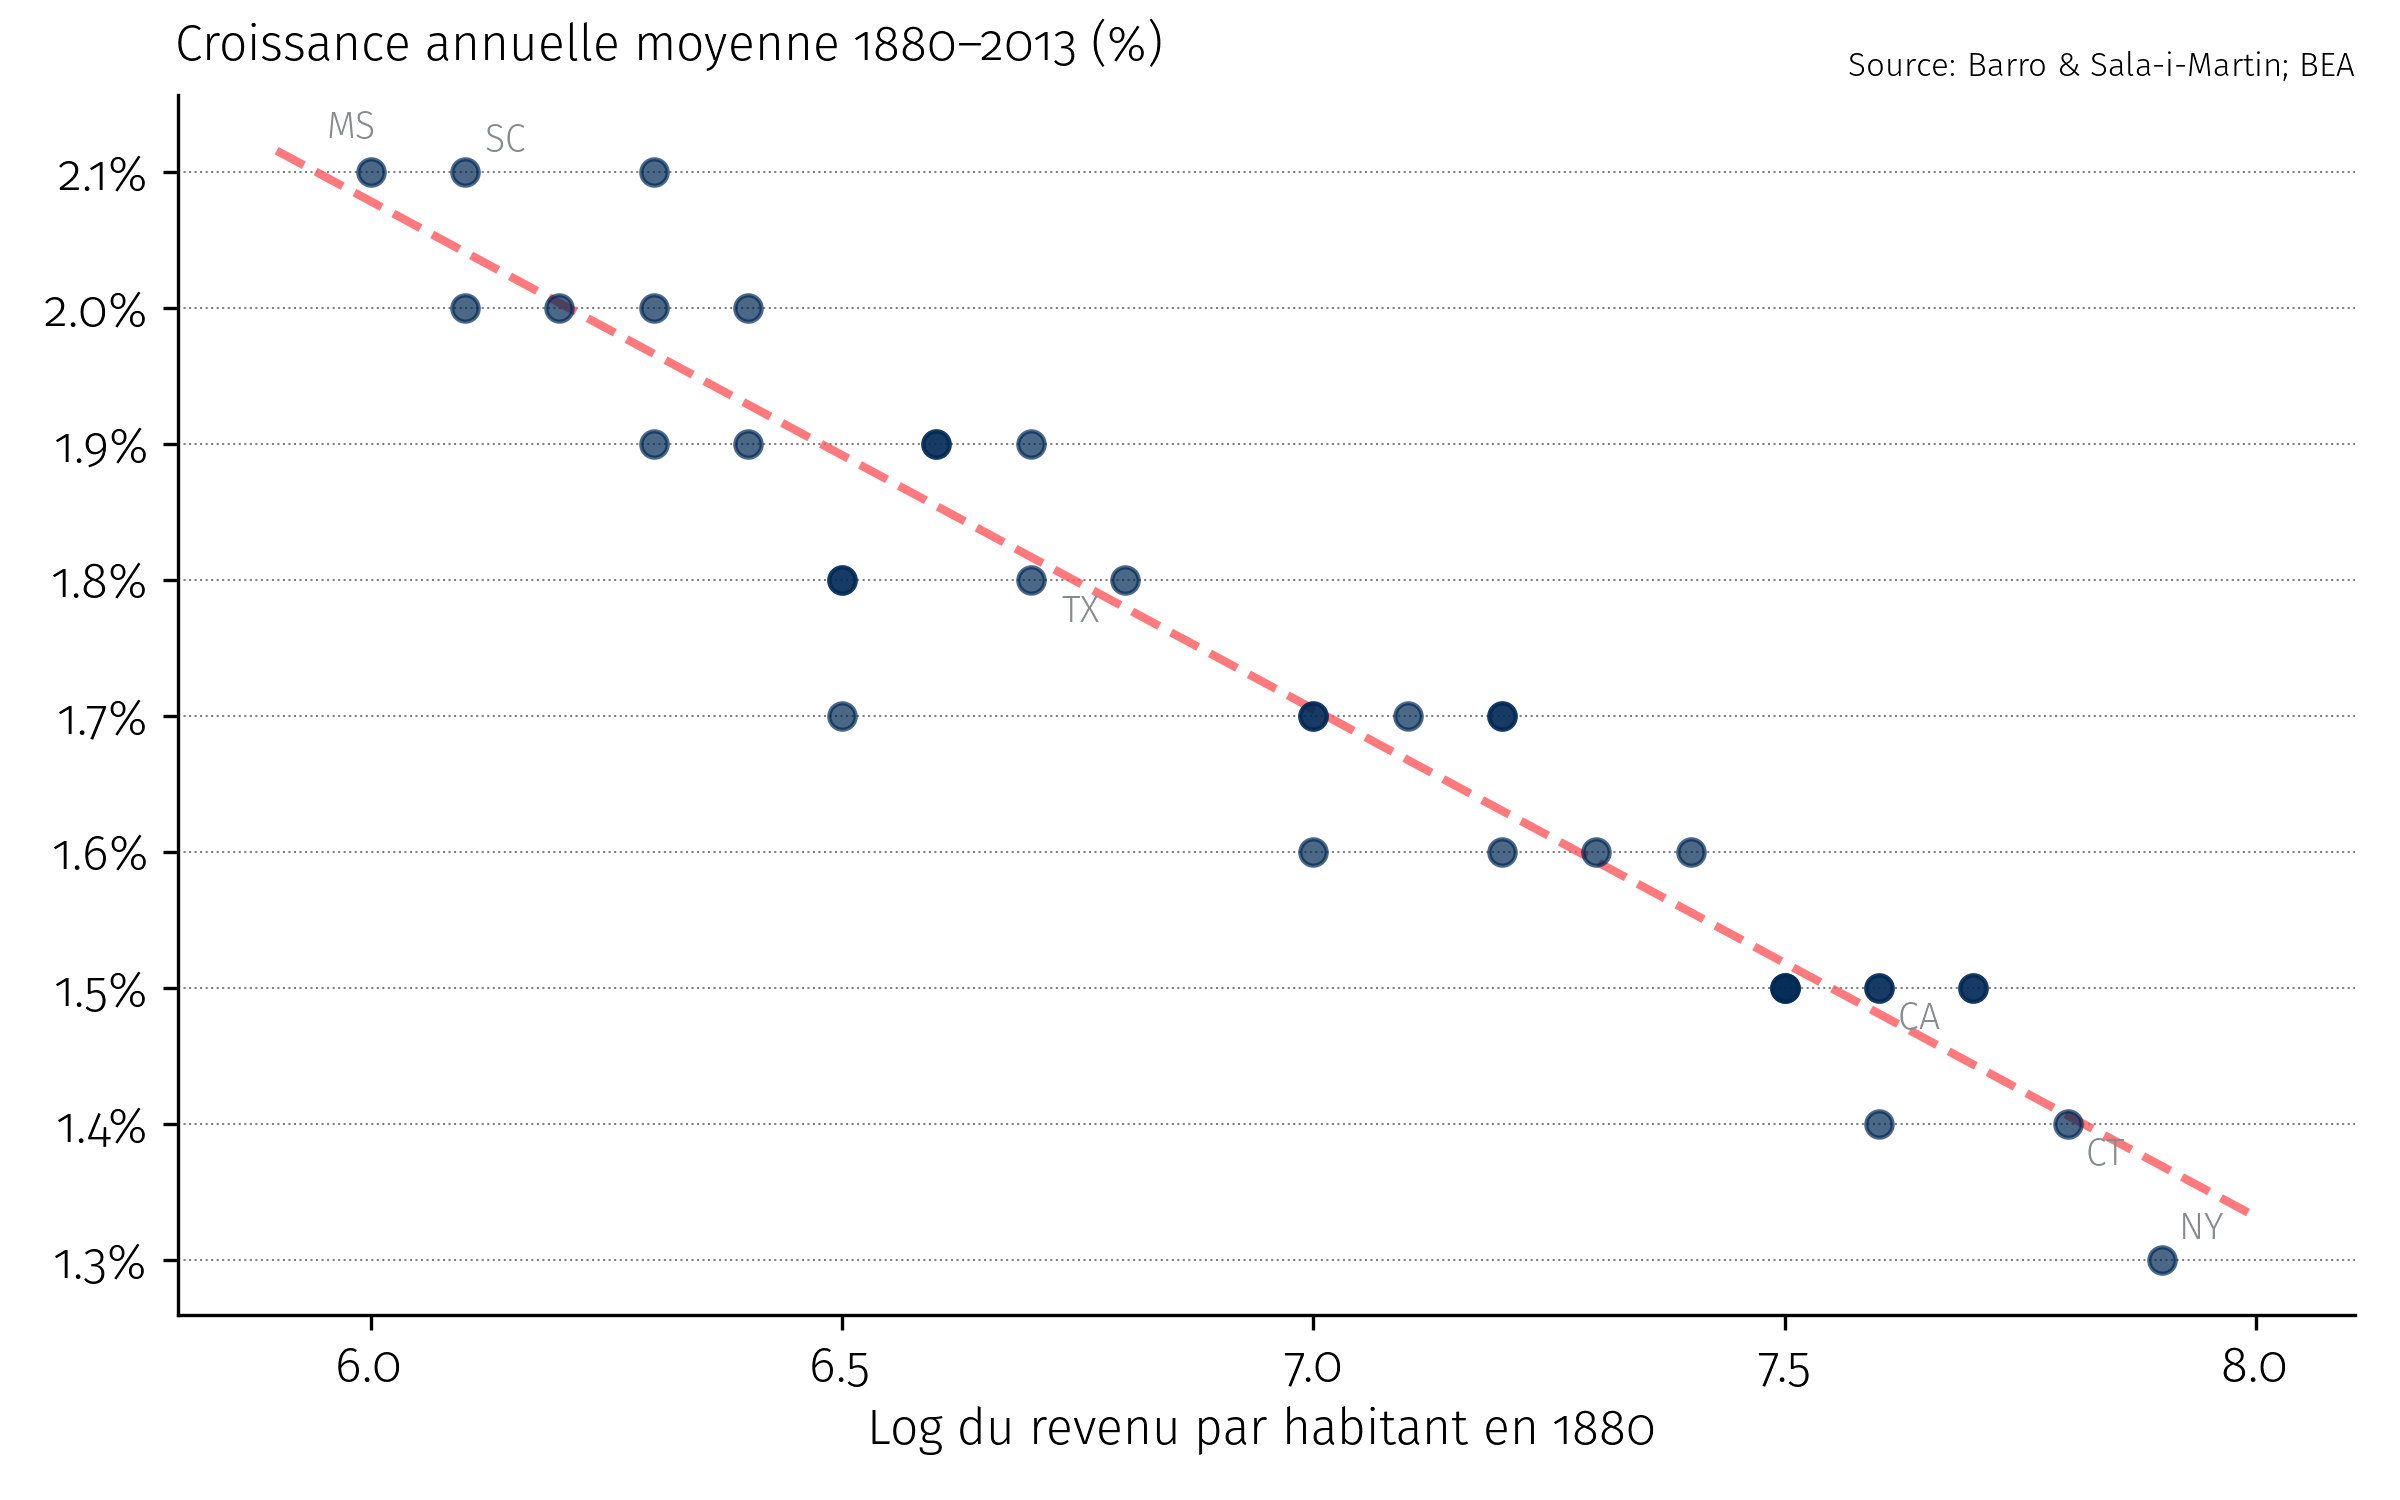
\includegraphics[width=0.9\textwidth, height=0.78\textheight, keepaspectratio]{convergence_us_states.png}
   \end{figure}
\end{frame}

\begin{frame}{Convergence entre économies avancées}
   \vspace{-0.2cm}
   \begin{figure}
      \centering
      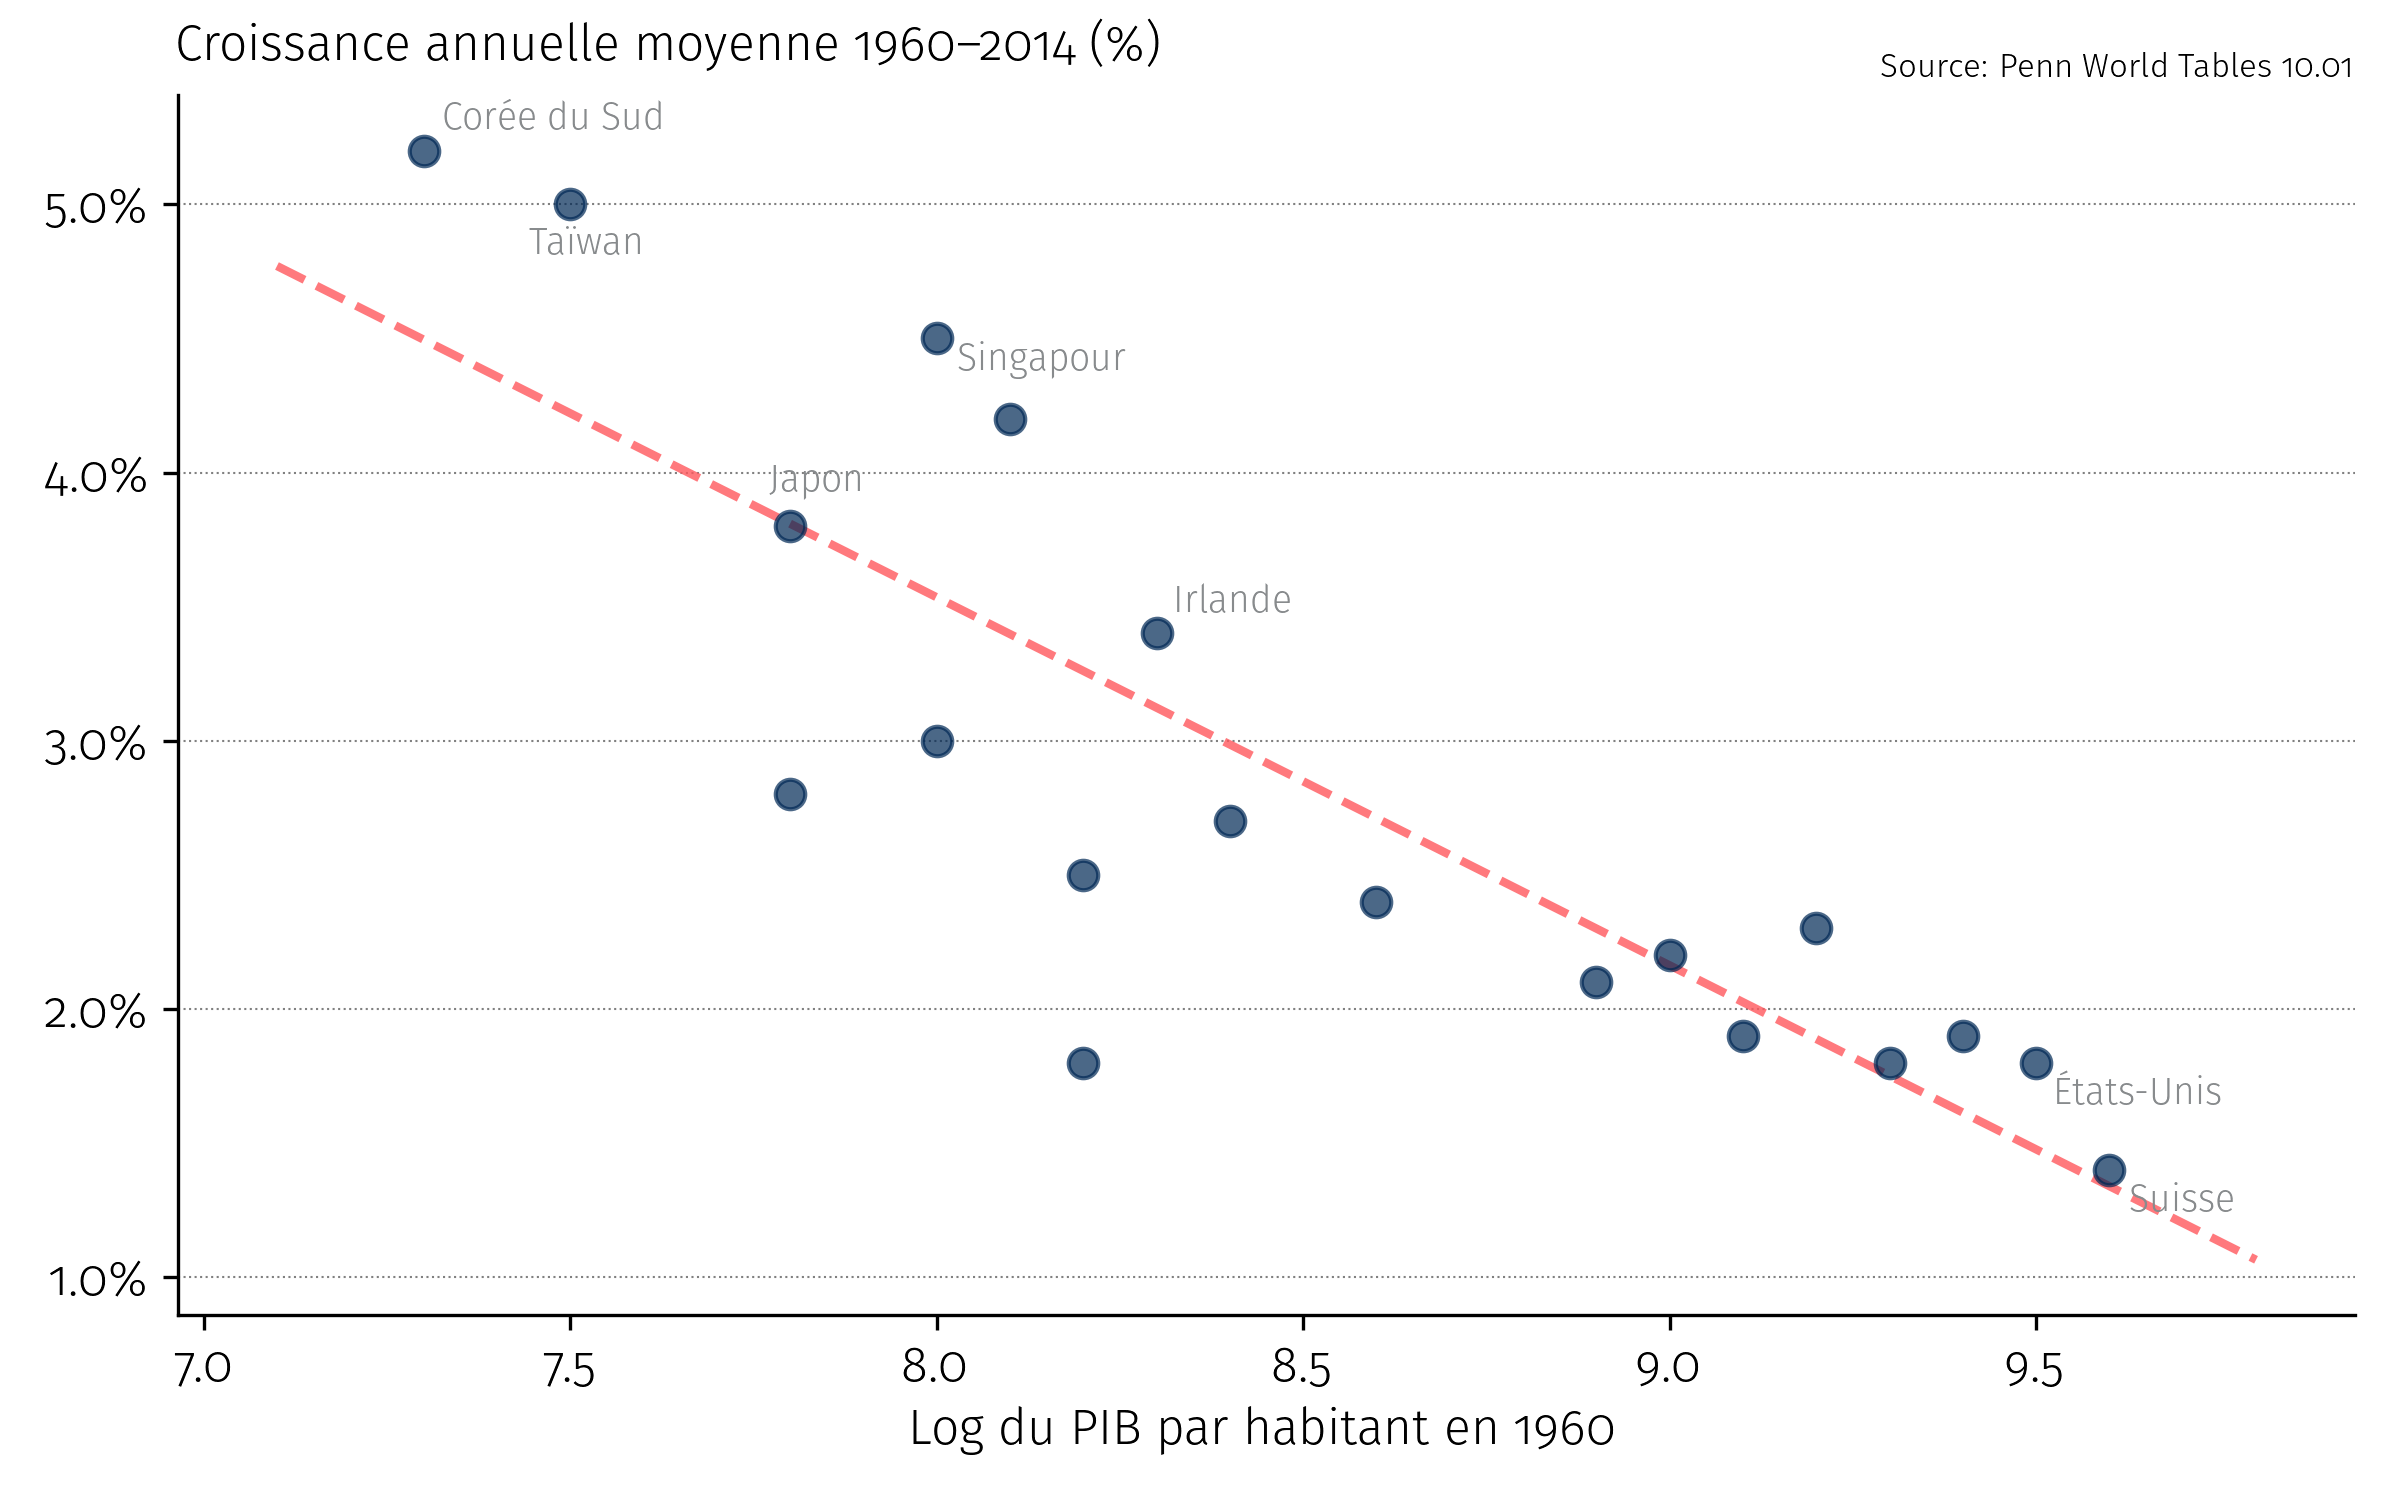
\includegraphics[width=0.9\textwidth, height=0.78\textheight, keepaspectratio]{convergence_oecd.png}
   \end{figure}
\end{frame}

\begin{frame}[t]{Convergence mondiale : un portrait nuancé}
   \vspace{-0.2cm}
   \begin{figure}
      \centering
      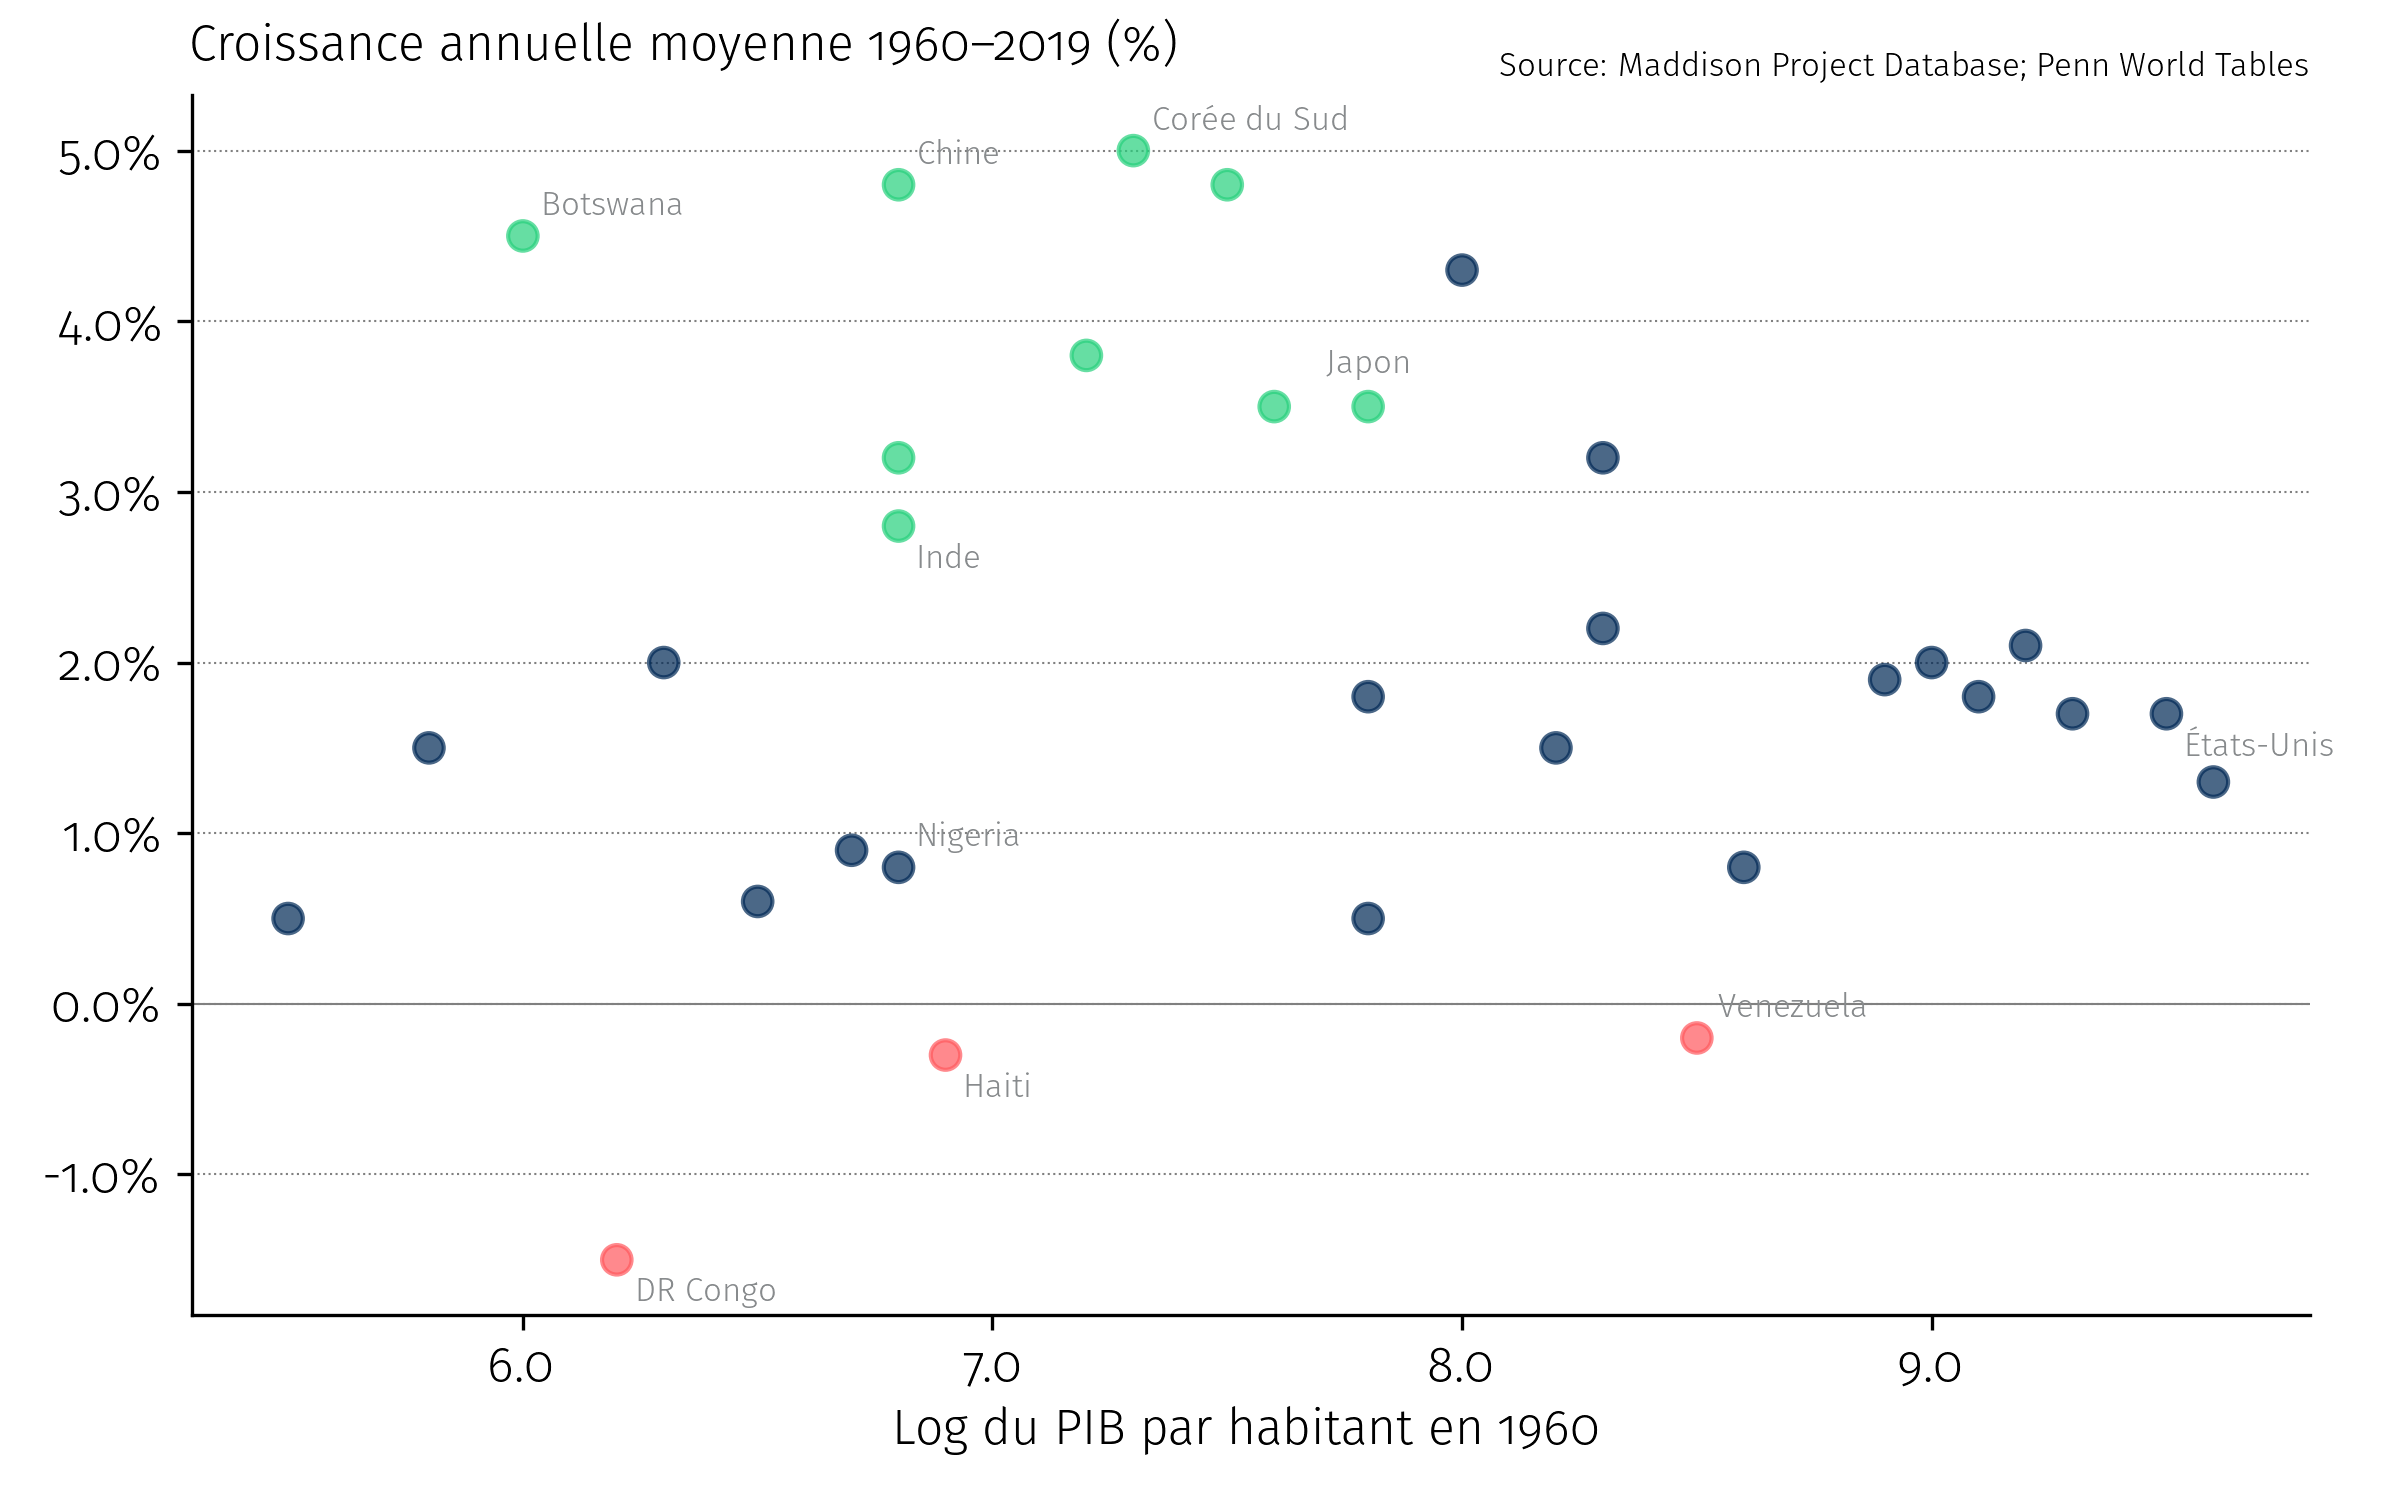
\includegraphics[width=0.85\textwidth, height=0.55\textheight, keepaspectratio]{convergence_global.png}
   \end{figure}
   \vspace{-0.3cm}
   \begin{warning}
      \small La convergence \textbf{n'est pas automatique}. Elle s'observe entre économies aux paramètres similaires (\textbf{convergence conditionnelle}), mais pas nécessairement à l'échelle mondiale.
   \end{warning}
\end{frame}

% --- Korea satellite photo ---
{
\setbeamertemplate{footline}{}
\begin{frame}[plain]
   \begin{tikzpicture}[remember picture, overlay]
      \node[anchor=center, inner sep=0pt] at (current page.center) {%
         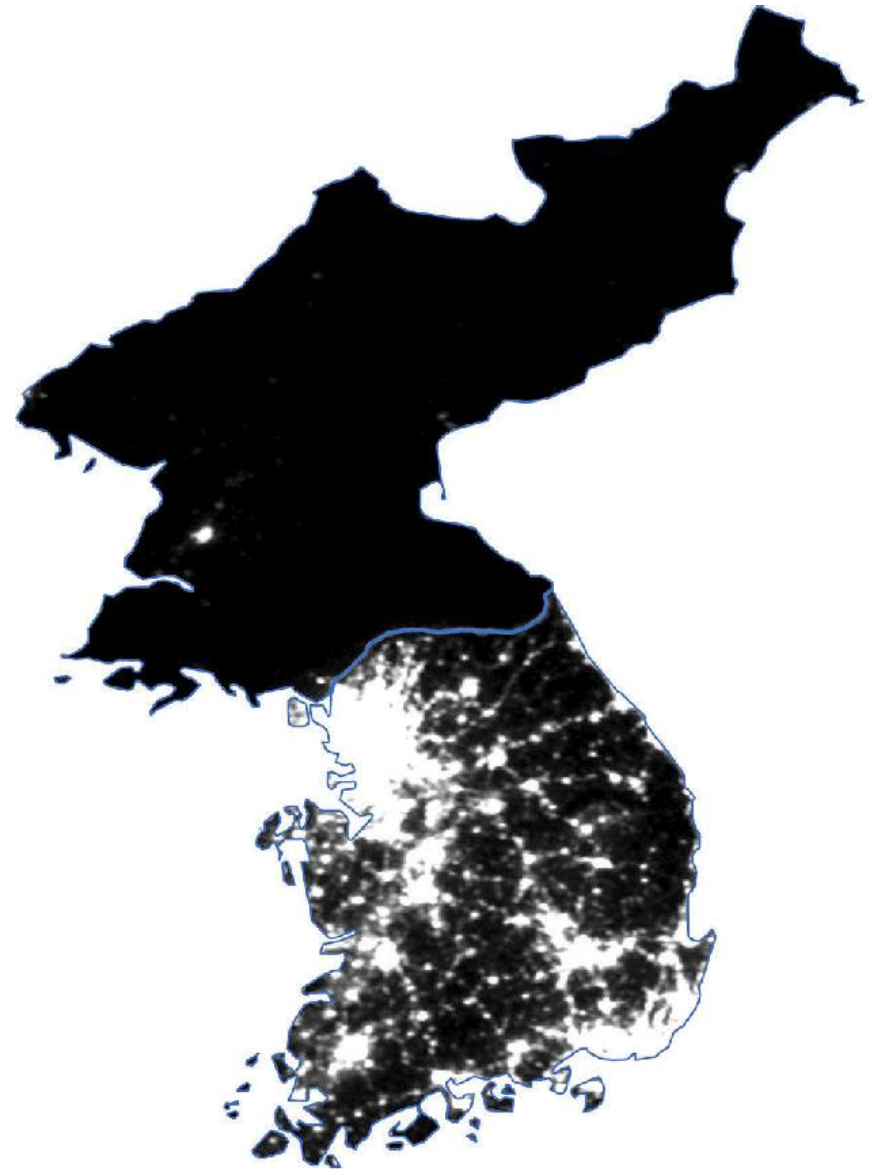
\includegraphics[width=\paperwidth, height=\paperheight, keepaspectratio]{korea_satellite.png}%
      };
      \node[anchor=south, fill=black, fill opacity=0.6, text opacity=1, inner sep=8pt,
            text width=0.7\paperwidth, align=center]
         at ([yshift=0.5cm]current page.south)
         {\normalsize\textcolor{white}{Corée du Nord vs Corée du Sud --- même géographie, même culture, même histoire jusqu'en 1945. \textbf{Des institutions radicalement différentes.}}};
   \end{tikzpicture}
\end{frame}
}

\begin{frame}[t]{Pourquoi certains pays ne convergent-ils pas?}
   \small
   Dans le modèle de Solow, la convergence suppose des \textbf{paramètres identiques}. En réalité :
   \vspace{0.15cm}
   \begin{itemize}
      \setlength\itemsep{0.15cm}
      \item \textbf{Institutions} différentes $\to$ différents $A$, $s$
      \item \textbf{Gouvernance} déficiente $\to$ faible $s$ effectif (corruption, détournement)
      \item \textbf{Conflits} et instabilité $\to$ destruction de capital récurrente
      \item \textbf{Géographie} et santé $\to$ productivité réduite
   \end{itemize}
   \vspace{0.15cm}
   Même modèle de Solow, mais des \textbf{paramètres différents} $\to$ des équilibres différents
   \vspace{0.1cm}
   \begin{bizimplication}
      Identifier les économies qui \textbf{convergent} (amélioration institutionnelle, ouverture, stabilité) = identifier les opportunités d'investissement de long terme.
   \end{bizimplication}
\end{frame}

% ============================================================================
\begin{frame}{Plan}
   \begin{enumerate}
      \setlength\itemsep{0.25cm}
      \item {\color{gray!50}La croissance est un phénomène récent}
      \item {\color{gray!50}La fonction de production}
      \item {\color{gray!50}Décomposer la croissance}
      \item {\color{gray!50}Le modèle de Solow}
      \item {\color{gray!50}Convergence}
      \item \textbf{Le vrai moteur de la croissance}
      \item Le casse-tête canadien de la productivité
      \item Croissance et environnement
   \end{enumerate}
\end{frame}

% ============================================================================
\sectionframe{Le vrai moteur de la croissance}
% ============================================================================

\begin{frame}[t]{Le résultat négatif de Solow}
   À l'état stationnaire de la baignoire, $K/N$ est stable $\to$ $Y/N$ est stable.
   \vspace{0.3cm}

   \textbf{Problème :} on observe une croissance \textit{soutenue} du PIB par habitant depuis 200+ ans!
   \vspace{0.3cm}

   \begin{itemize}
      \setlength\itemsep{0.2cm}
      \item Le hockey stick n'est \textbf{pas} expliqué par le capital seul
      \item L'accumulation de capital a des rendements décroissants
      \item Quelque chose d'\textbf{autre} doit tirer la croissance de long terme
   \end{itemize}
   \vspace{0.3cm}
   Qu'est-ce qui manque au modèle?
\end{frame}

\begin{frame}[t]{Le seul moteur de long terme : la productivité}
   \textbf{Quand $A$ augmente}, toute la fonction de production se déplace vers le haut :
   \vspace{0.2cm}
   \begin{itemize}
      \setlength\itemsep{0.15cm}
      \item Chaque unité de $K$ et $N$ produit \textbf{davantage}
      \item L'investissement par travailleur ($s \cdot Y/N$) augmente
      \item La baignoire \guillemotleft~grossit~\guillemotright\ --- un \textbf{nouvel} état stationnaire, plus élevé
      \item Si $A$ croît en permanence, $K/N$ et $Y/N$ croissent en permanence
   \end{itemize}
   \vspace{0.2cm}
   \begin{keyinsight}
      La \textbf{technologie} (au sens large : PTF) est le seul facteur capable de soutenir une croissance \textit{indéfinie} du niveau de vie. Le capital suit, mais ne mène pas.
   \end{keyinsight}
\end{frame}

\begin{frame}[t]{Les idées ne sont pas comme les objets}
   \small
   \textbf{Non-rivalité des idées :} quand j'utilise le calcul différentiel, cela ne vous empêche pas de l'utiliser. Personne n'est \guillemotleft~privé~\guillemotright\ d'une idée parce qu'un autre s'en sert.
   \vspace{0.2cm}

   \textbf{Conséquence pour la production :}
   \vspace{0.1cm}
   \begin{itemize}
      \setlength\itemsep{0.1cm}
      \item Pour les \textbf{objets} (K, N) : rendements d'échelle constants ($2K + 2N \to 2Y$)
      \item Pour les \textbf{objets + idées} : rendements d'échelle \textbf{croissants}!
   \end{itemize}
   \vspace{0.15cm}
   \begin{keyinsight}
      Pour cloner une usine, il faut doubler les machines et les travailleurs --- mais \textbf{pas} réinventer les plans techniques. Les idées se répliquent à coût nul, ce qui crée des rendements croissants.
   \end{keyinsight}
\end{frame}

\begin{frame}[t]{Qu'est-ce qui fait croître $A$?}
   \small
   La productivité n'est pas seulement la Silicon Valley. Elle englobe :
   \vspace{0.15cm}
   \begin{itemize}
      \setlength\itemsep{0.1cm}
      \item \textbf{Innovation technologique} : R\&D, brevets, nouvelles technologies
      \item \textbf{Éducation et capital humain} : qualité de la main-d'œuvre
      \item \textbf{Institutions} : état de droit, droits de propriété, concurrence
      \item \textbf{Ouverture commerciale} : diffusion des idées, spécialisation
      \item \textbf{Efficacité organisationnelle} : management, logistique, allocation des ressources
   \end{itemize}
   \vspace{0.1cm}
   \begin{bizimplication}
      Pour une entreprise, améliorer la productivité passe autant par de meilleures \textbf{pratiques de gestion} que par l'adoption de nouvelles technologies.
   \end{bizimplication}
\end{frame}

\begin{frame}[t]{Le rôle crucial des institutions}
   \small
   \textbf{Acemoglu, Johnson \& Robinson} (Prix Nobel 2024) : les institutions coloniales expliquent les différences persistantes de revenus.
   \vspace{0.15cm}
   \begin{itemize}
      \setlength\itemsep{0.1cm}
      \item \textbf{Institutions inclusives :} droits de propriété, état de droit, concurrence $\to$ innovation, investissement
      \item \textbf{Institutions extractives :} monopole, corruption, expropriation $\to$ stagnation
   \end{itemize}
   \vspace{0.15cm}
   \textbf{Mauvaise allocation des ressources :}
   \vspace{0.1cm}
   \begin{itemize}
      \setlength\itemsep{0.1cm}
      \item Quand le produit marginal du capital diffère entre entreprises, \textbf{réallouer} le capital (des entreprises peu productives vers les productives) augmente la PTF \textbf{sans nouvel investissement}
      \item Cette mauvaise allocation est un frein majeur dans les pays en développement
   \end{itemize}
\end{frame}

\begin{frame}{Sommes-nous à bout de souffle?}
   \begin{figure}
      \centering
      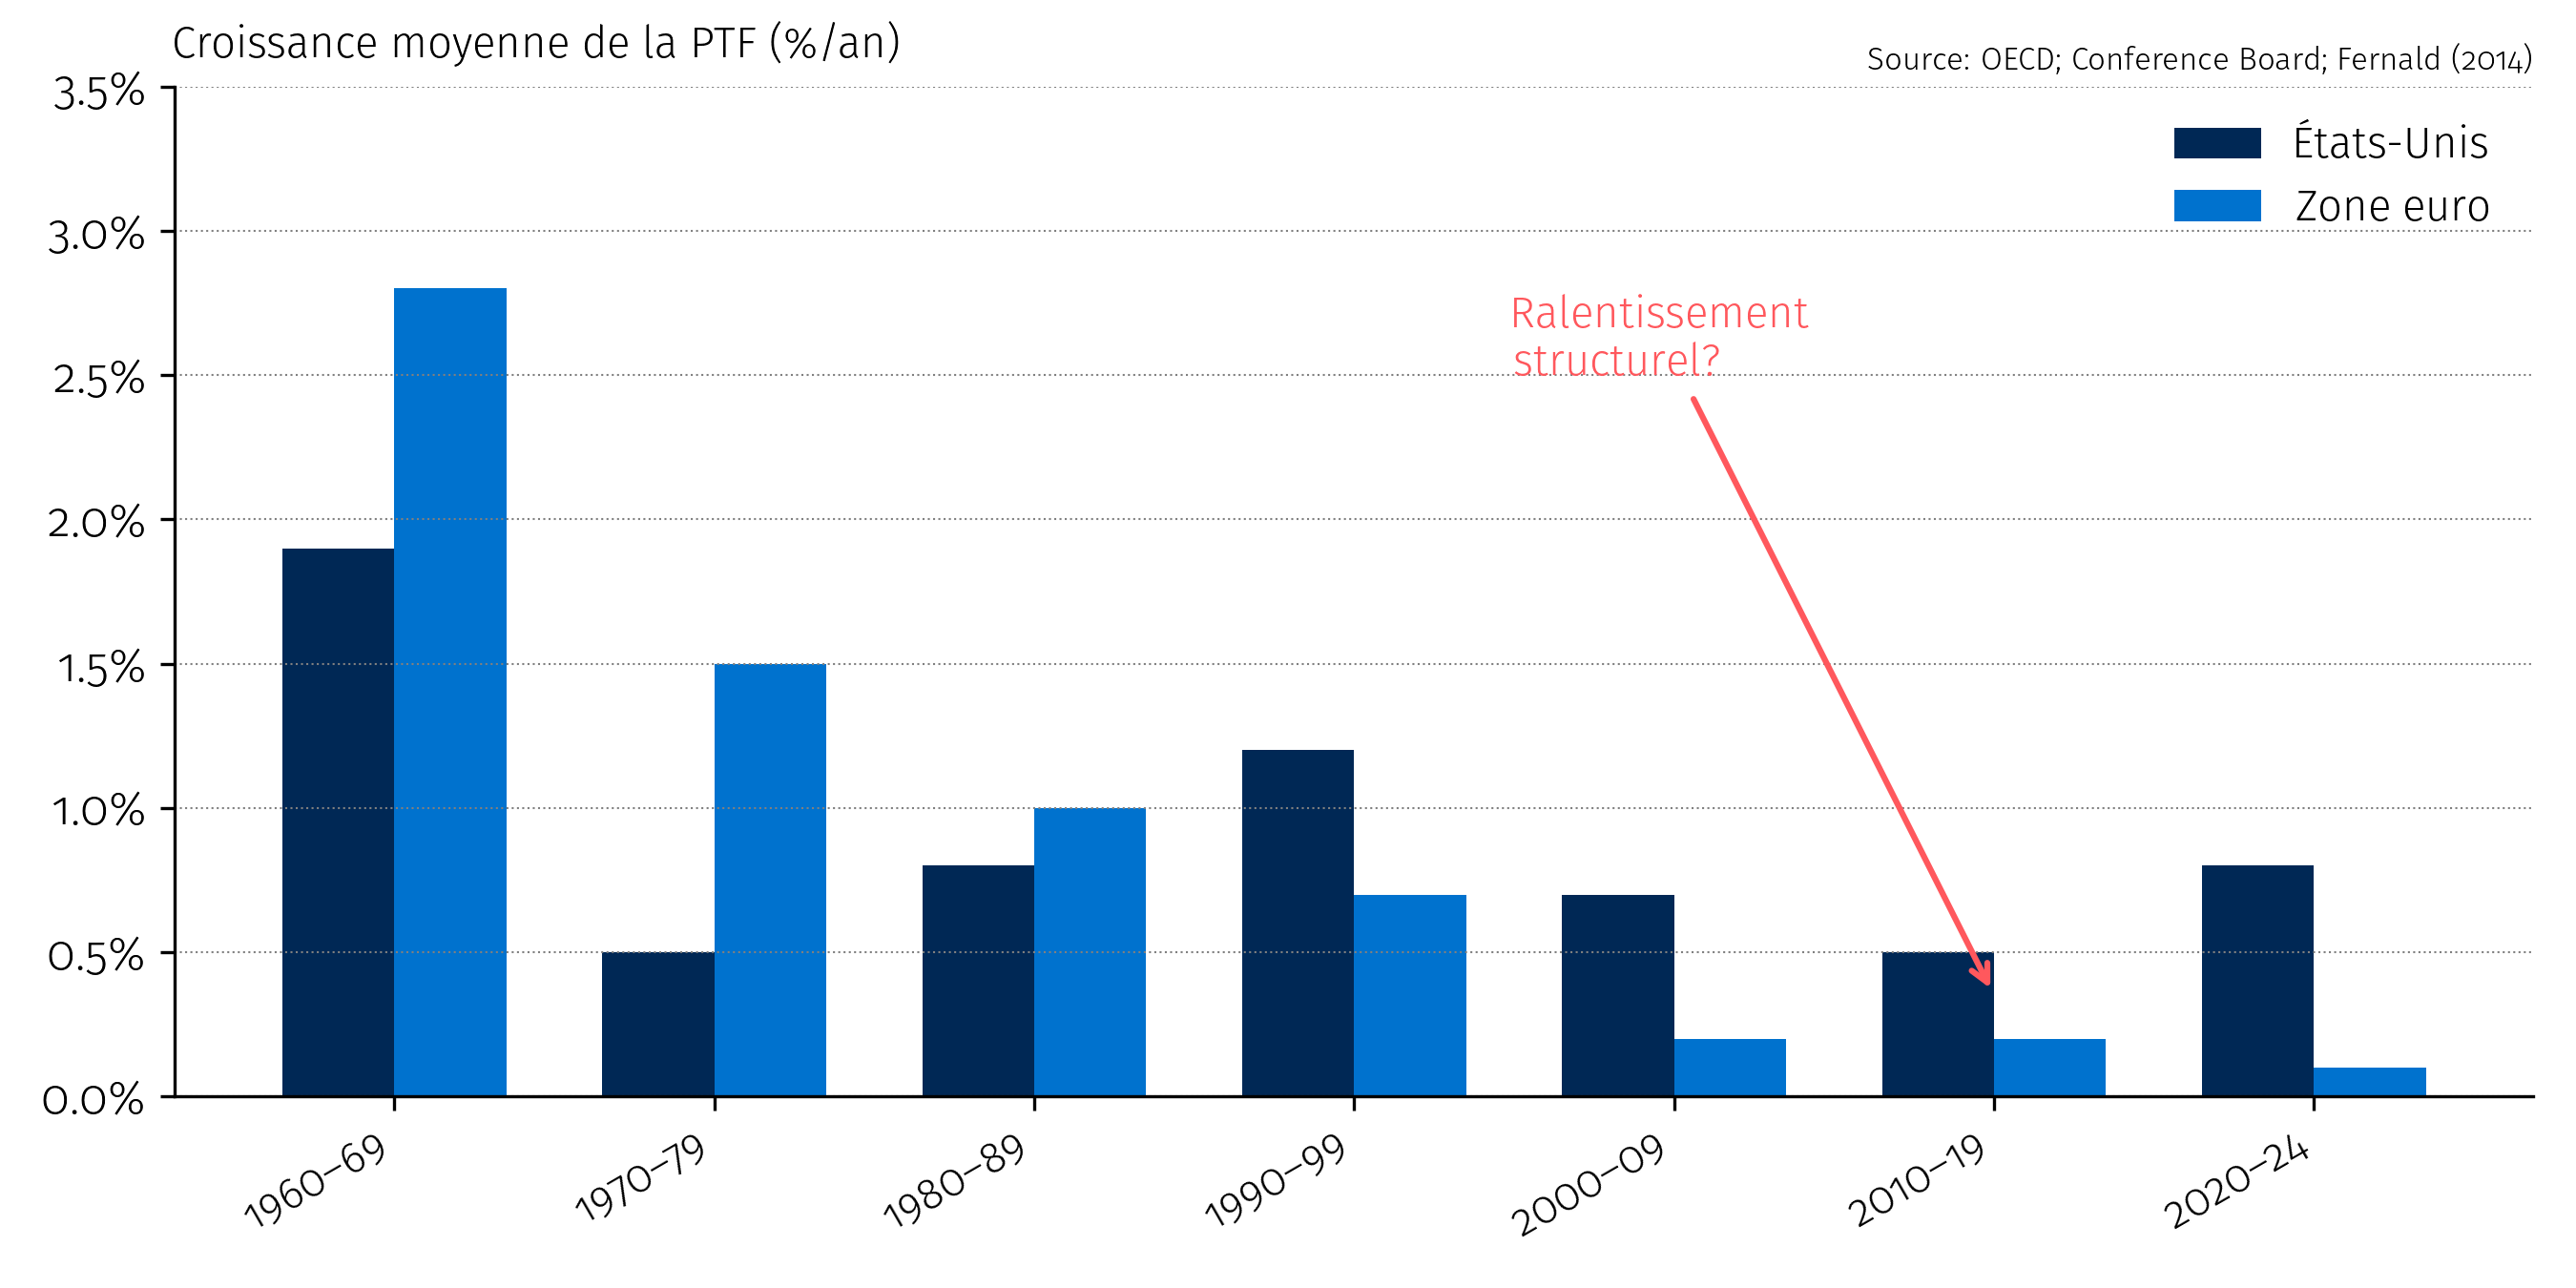
\includegraphics[width=0.9\textwidth]{tfp_growth_advanced.png}
   \end{figure}
   \vspace{-0.2cm}
   \footnotesize La croissance de la PTF ralentit dans les économies avancées depuis les années 2000. Mais l'IA et l'innovation dans les marchés émergents offrent des raisons d'être optimistes.
\end{frame}

% ============================================================================
\begin{frame}{Plan}
   \begin{enumerate}
      \setlength\itemsep{0.25cm}
      \item {\color{gray!50}La croissance est un phénomène récent}
      \item {\color{gray!50}La fonction de production}
      \item {\color{gray!50}Décomposer la croissance}
      \item {\color{gray!50}Le modèle de Solow}
      \item {\color{gray!50}Convergence}
      \item {\color{gray!50}Le vrai moteur de la croissance}
      \item \textbf{Le casse-tête canadien de la productivité}
      \item Croissance et environnement
   \end{enumerate}
\end{frame}

% ============================================================================
\sectionframe{Le casse-tête canadien de la productivité}
% ============================================================================

\begin{frame}{Le Canada décroche}
   \vspace{-0.2cm}
   \begin{figure}
      \centering
      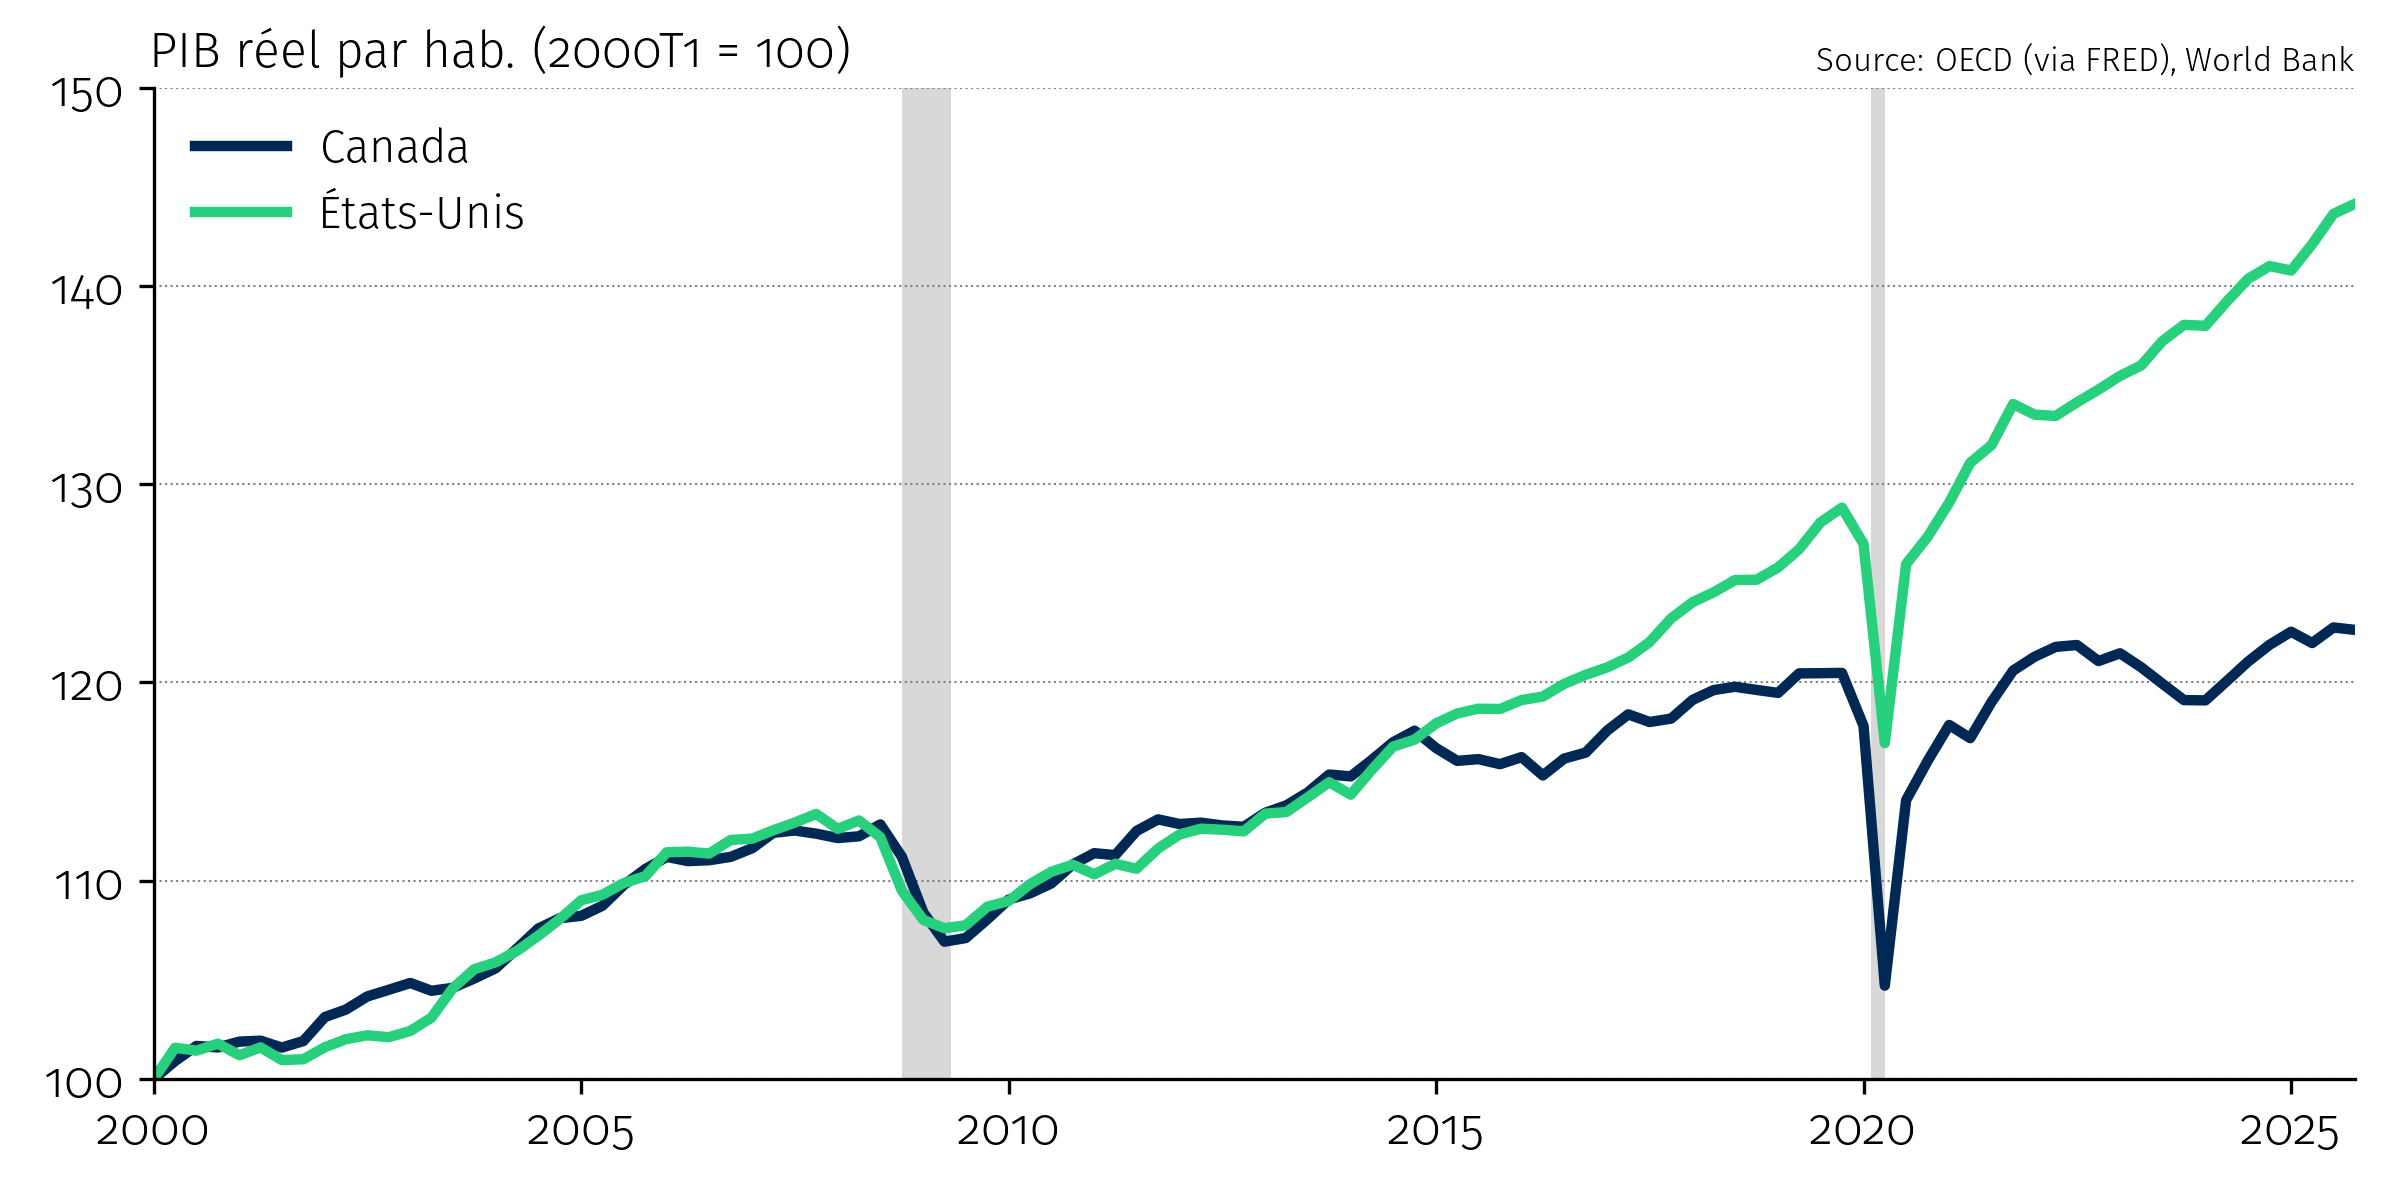
\includegraphics[width=0.9\textwidth, height=0.55\textheight, keepaspectratio]{gdp_per_capita_canada_usa.png}
   \end{figure}
   \vspace{-0.3cm}
   Le PIB par habitant du Canada \textbf{diminue} par rapport aux États-Unis depuis $\sim$2015. En 2024, l'écart est à son plus haut niveau depuis les années 1980.
\end{frame}

\begin{frame}[t]{Un problème d'investissement?}
   \vspace{-0.2cm}
   \begin{figure}
      \centering
      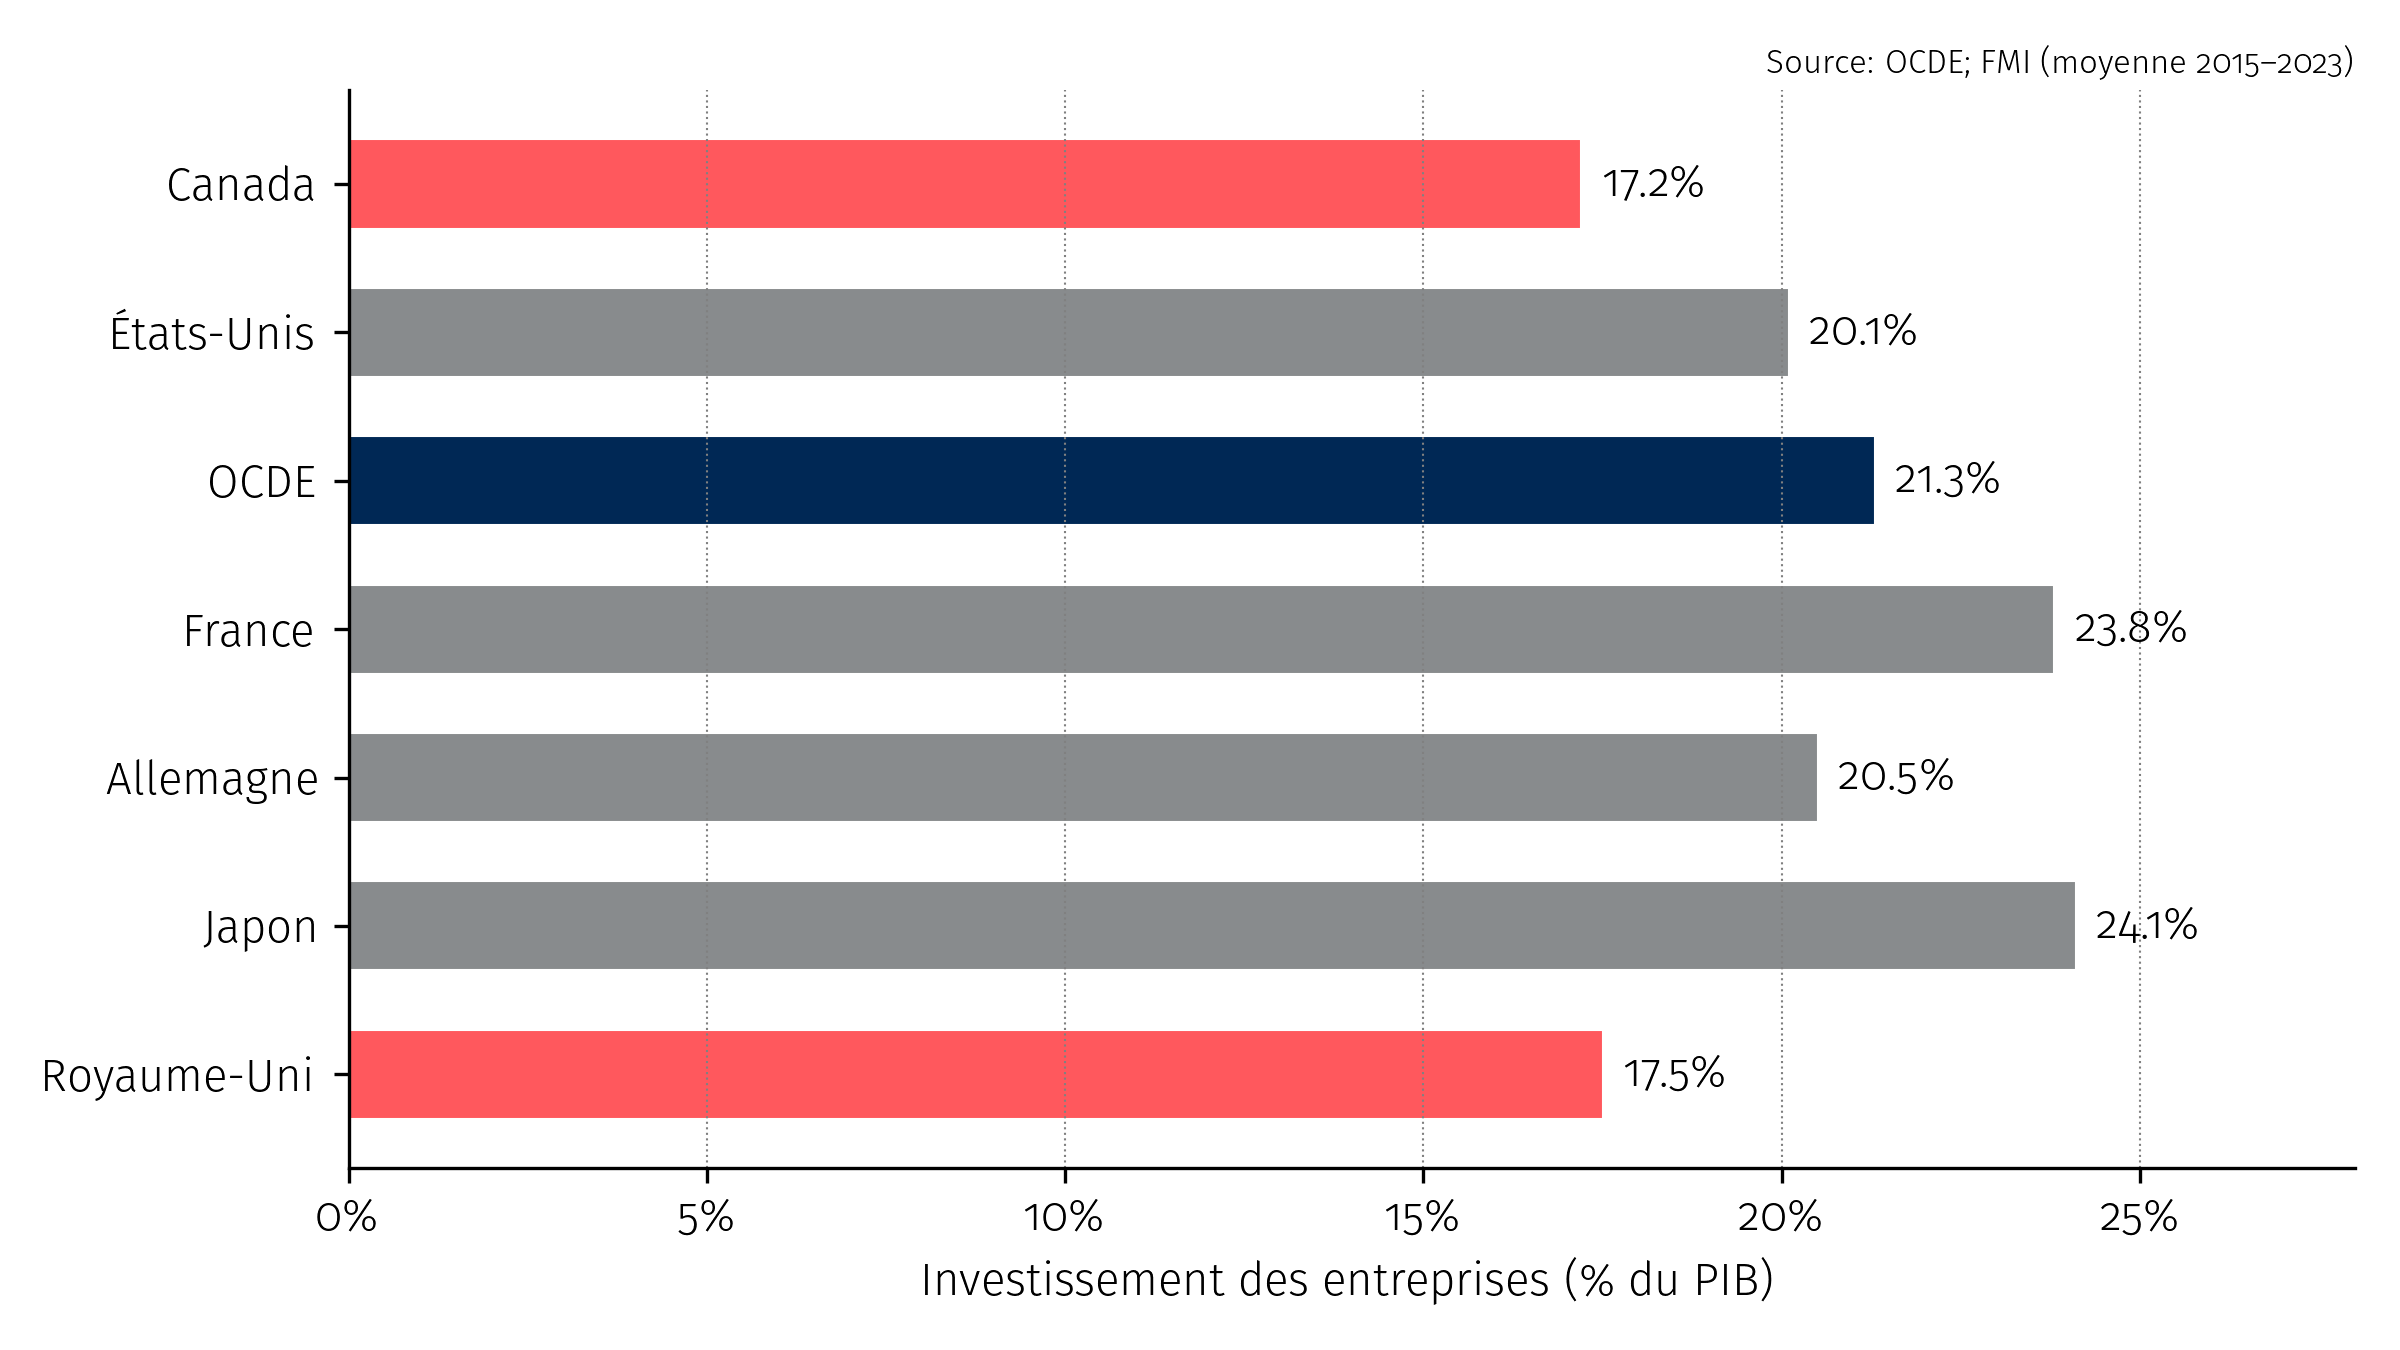
\includegraphics[width=0.9\textwidth, height=0.55\textheight, keepaspectratio]{oecd_business_investment.png}
   \end{figure}
   \vspace{-0.3cm}
   L'investissement des entreprises canadiennes en \% du PIB est \textbf{systématiquement inférieur} à celui des États-Unis et de la moyenne OCDE. Moins de capital $\to$ moins de productivité.
\end{frame}

\begin{frame}[t]{Productivité : le diagnostic}
   \vspace{-0.2cm}
   \begin{figure}
      \centering
      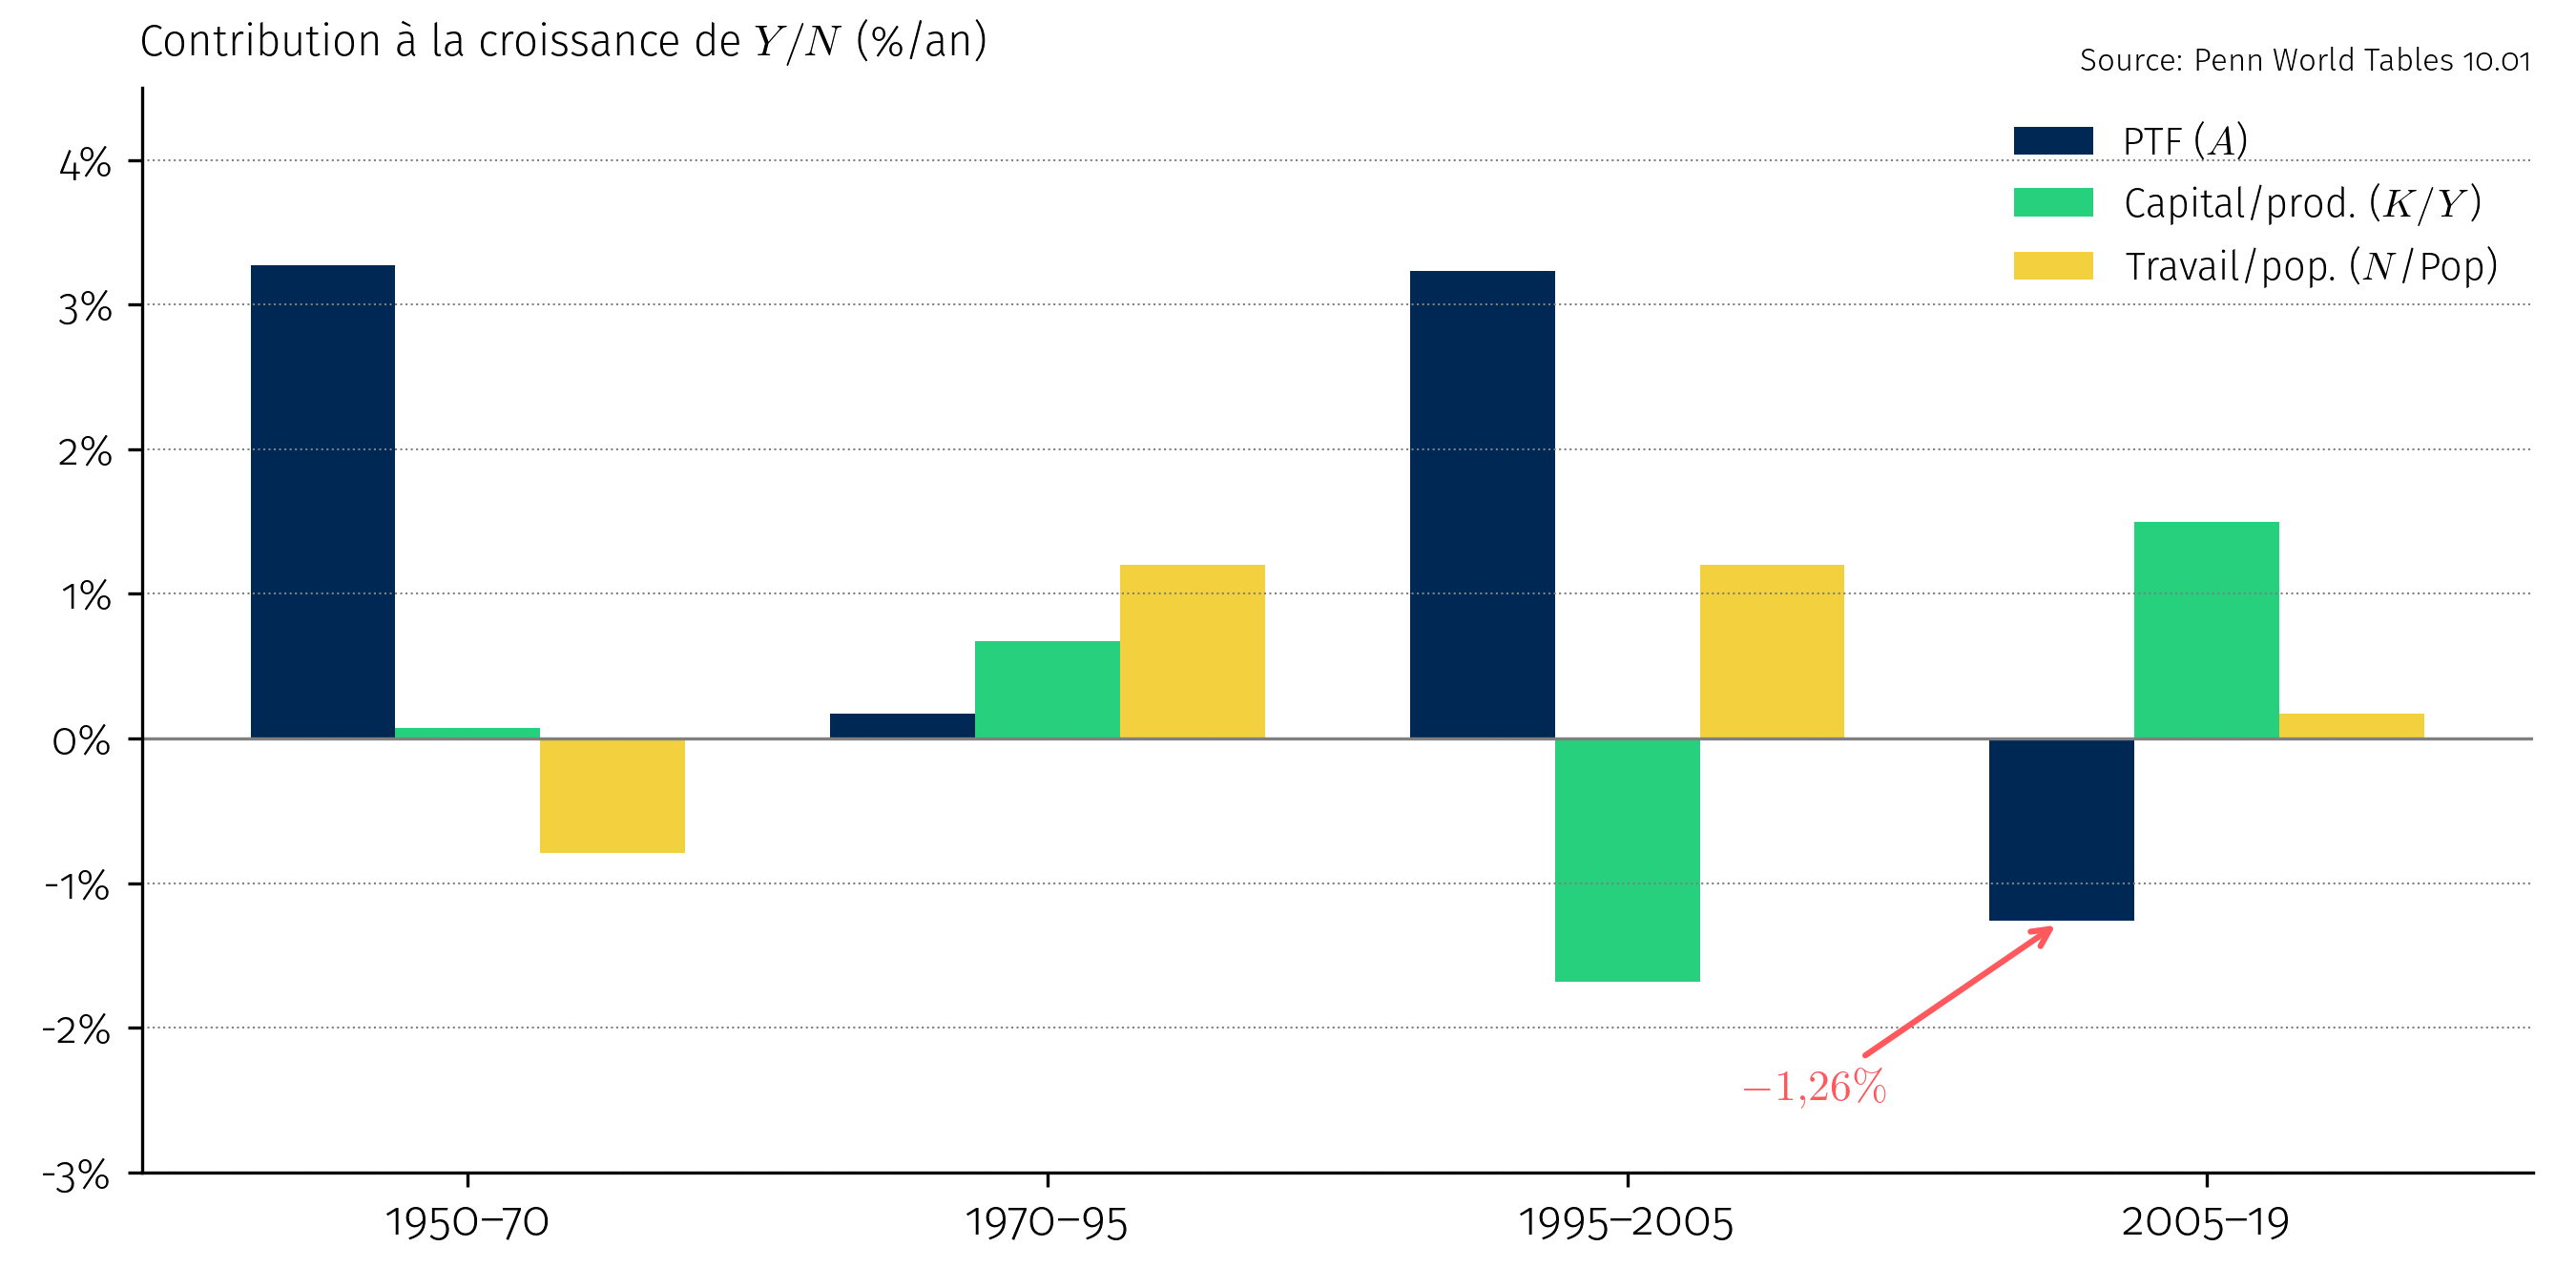
\includegraphics[width=0.85\textwidth, height=0.5\textheight, keepaspectratio]{canada_productivity_growth.png}
   \end{figure}
   \vspace{-0.3cm}
   \begin{warning}
      \footnotesize De 2005 à 2019, la croissance de la PTF au Canada a été \textbf{négative} ($-1{,}26\,\%$/an). Le Canada ne souffre pas seulement d'un manque de capital --- il souffre d'un problème de \textbf{productivité}.
   \end{warning}
\end{frame}

\begin{frame}[t]{Le cercle vicieux}
   \small
   Le Canada est pris dans un cercle vicieux :
   \vspace{0.2cm}
   \begin{center}
   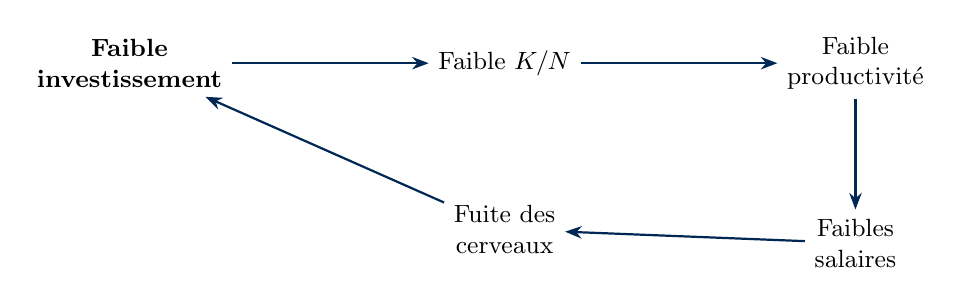
\begin{tikzpicture}[
      node distance=1.4cm and 2.5cm,
      every node/.style={align=center, font=\small},
      arr/.style={-{Stealth[length=6pt]}, thick, HECnavy}
   ]
      \node (invest) {\textbf{Faible}\\\textbf{investissement}};
      \node (kn) [right=of invest] {Faible $K/N$};
      \node (prod) [right=of kn] {Faible\\productivité};
      \node (wages) [below=of prod] {Faibles\\salaires};
      \node (brain) [below=of kn] {Fuite des\\cerveaux};
      \draw[arr] (invest) -- (kn);
      \draw[arr] (kn) -- (prod);
      \draw[arr] (prod) -- (wages);
      \draw[arr] (wages) -- (brain);
      \draw[arr] (brain) -- (invest);
   \end{tikzpicture}
   \end{center}
   \vspace{0.1cm}
   \begin{warning}
      Le Canada investit moins en R\&D que presque tous ses pairs du G7. En 2023 : 1,7\,\% du PIB vs 3,5\,\% aux États-Unis.
   \end{warning}
\end{frame}

\begin{frame}[t]{Que faire?}
   \small
   \begin{bizimplication}[Pistes de solution]
      \begin{itemize}
         \setlength\itemsep{0.1cm}
         \item \textbf{Incitatifs à la R\&D :} crédits d'impôt, financement de la recherche fondamentale
         \item \textbf{Immigration qualifiée :} attirer les talents en technologie et en sciences
         \item \textbf{Allègement réglementaire :} réduire les barrières à l'entrée et à la concurrence
         \item \textbf{Politique de concurrence :} briser les oligopoles (télécoms, banques, transport aérien)
      \end{itemize}
   \end{bizimplication}
   \vspace{0.15cm}
   Ce sont des solutions de \textbf{long terme}. Mais il y a une contrainte que nous n'avons pas encore abordée\ldots

   \vspace{0.15cm}
   $\to$ La croissance peut-elle être \textbf{soutenable} sur le plan environnemental?
\end{frame}

% ============================================================================
\begin{frame}{Plan}
   \begin{enumerate}
      \setlength\itemsep{0.25cm}
      \item {\color{gray!50}La croissance est un phénomène récent}
      \item {\color{gray!50}La fonction de production}
      \item {\color{gray!50}Décomposer la croissance}
      \item {\color{gray!50}Le modèle de Solow}
      \item {\color{gray!50}Convergence}
      \item {\color{gray!50}Le vrai moteur de la croissance}
      \item {\color{gray!50}Le casse-tête canadien de la productivité}
      \item \textbf{Croissance et environnement}
   \end{enumerate}
\end{frame}

% ============================================================================
\sectionframe{Croissance et environnement}
% ============================================================================

\begin{frame}[t]{L'identité de Kaya}
   \small
   Comment relier croissance économique et émissions de CO$_2$?
   \vspace{0.2cm}
   \begin{defbox}[Identité de Kaya]
      \begin{equation*}
         \underbrace{\text{CO}_2}_{\text{émissions}} \;=\; \underbrace{\text{Pop}}_{\text{population}} \;\times\; \underbrace{\frac{Y}{\text{Pop}}}_{\text{niveau de vie}} \;\times\; \underbrace{\frac{E}{Y}}_{\text{intensité}\\\text{énergétique}} \;\times\; \underbrace{\frac{\text{CO}_2}{E}}_{\text{intensité}\\\text{carbone}}
      \end{equation*}
   \end{defbox}
   \vspace{0.1cm}
   \textbf{Quatre leviers} pour réduire les émissions :
   \vspace{0.1cm}
   \begin{enumerate}
      \setlength\itemsep{0.1cm}
      \item Réduire la \textbf{population} (lent, éthiquement complexe)
      \item Réduire le \textbf{niveau de vie} (politiquement impossible)
      \item Réduire l'\textbf{intensité énergétique} (efficacité, sobriété)
      \item Réduire l'\textbf{intensité carbone} (renouvelables, nucléaire)
   \end{enumerate}
\end{frame}

\begin{frame}{Les quatre leviers}
   \begin{figure}
      \centering
      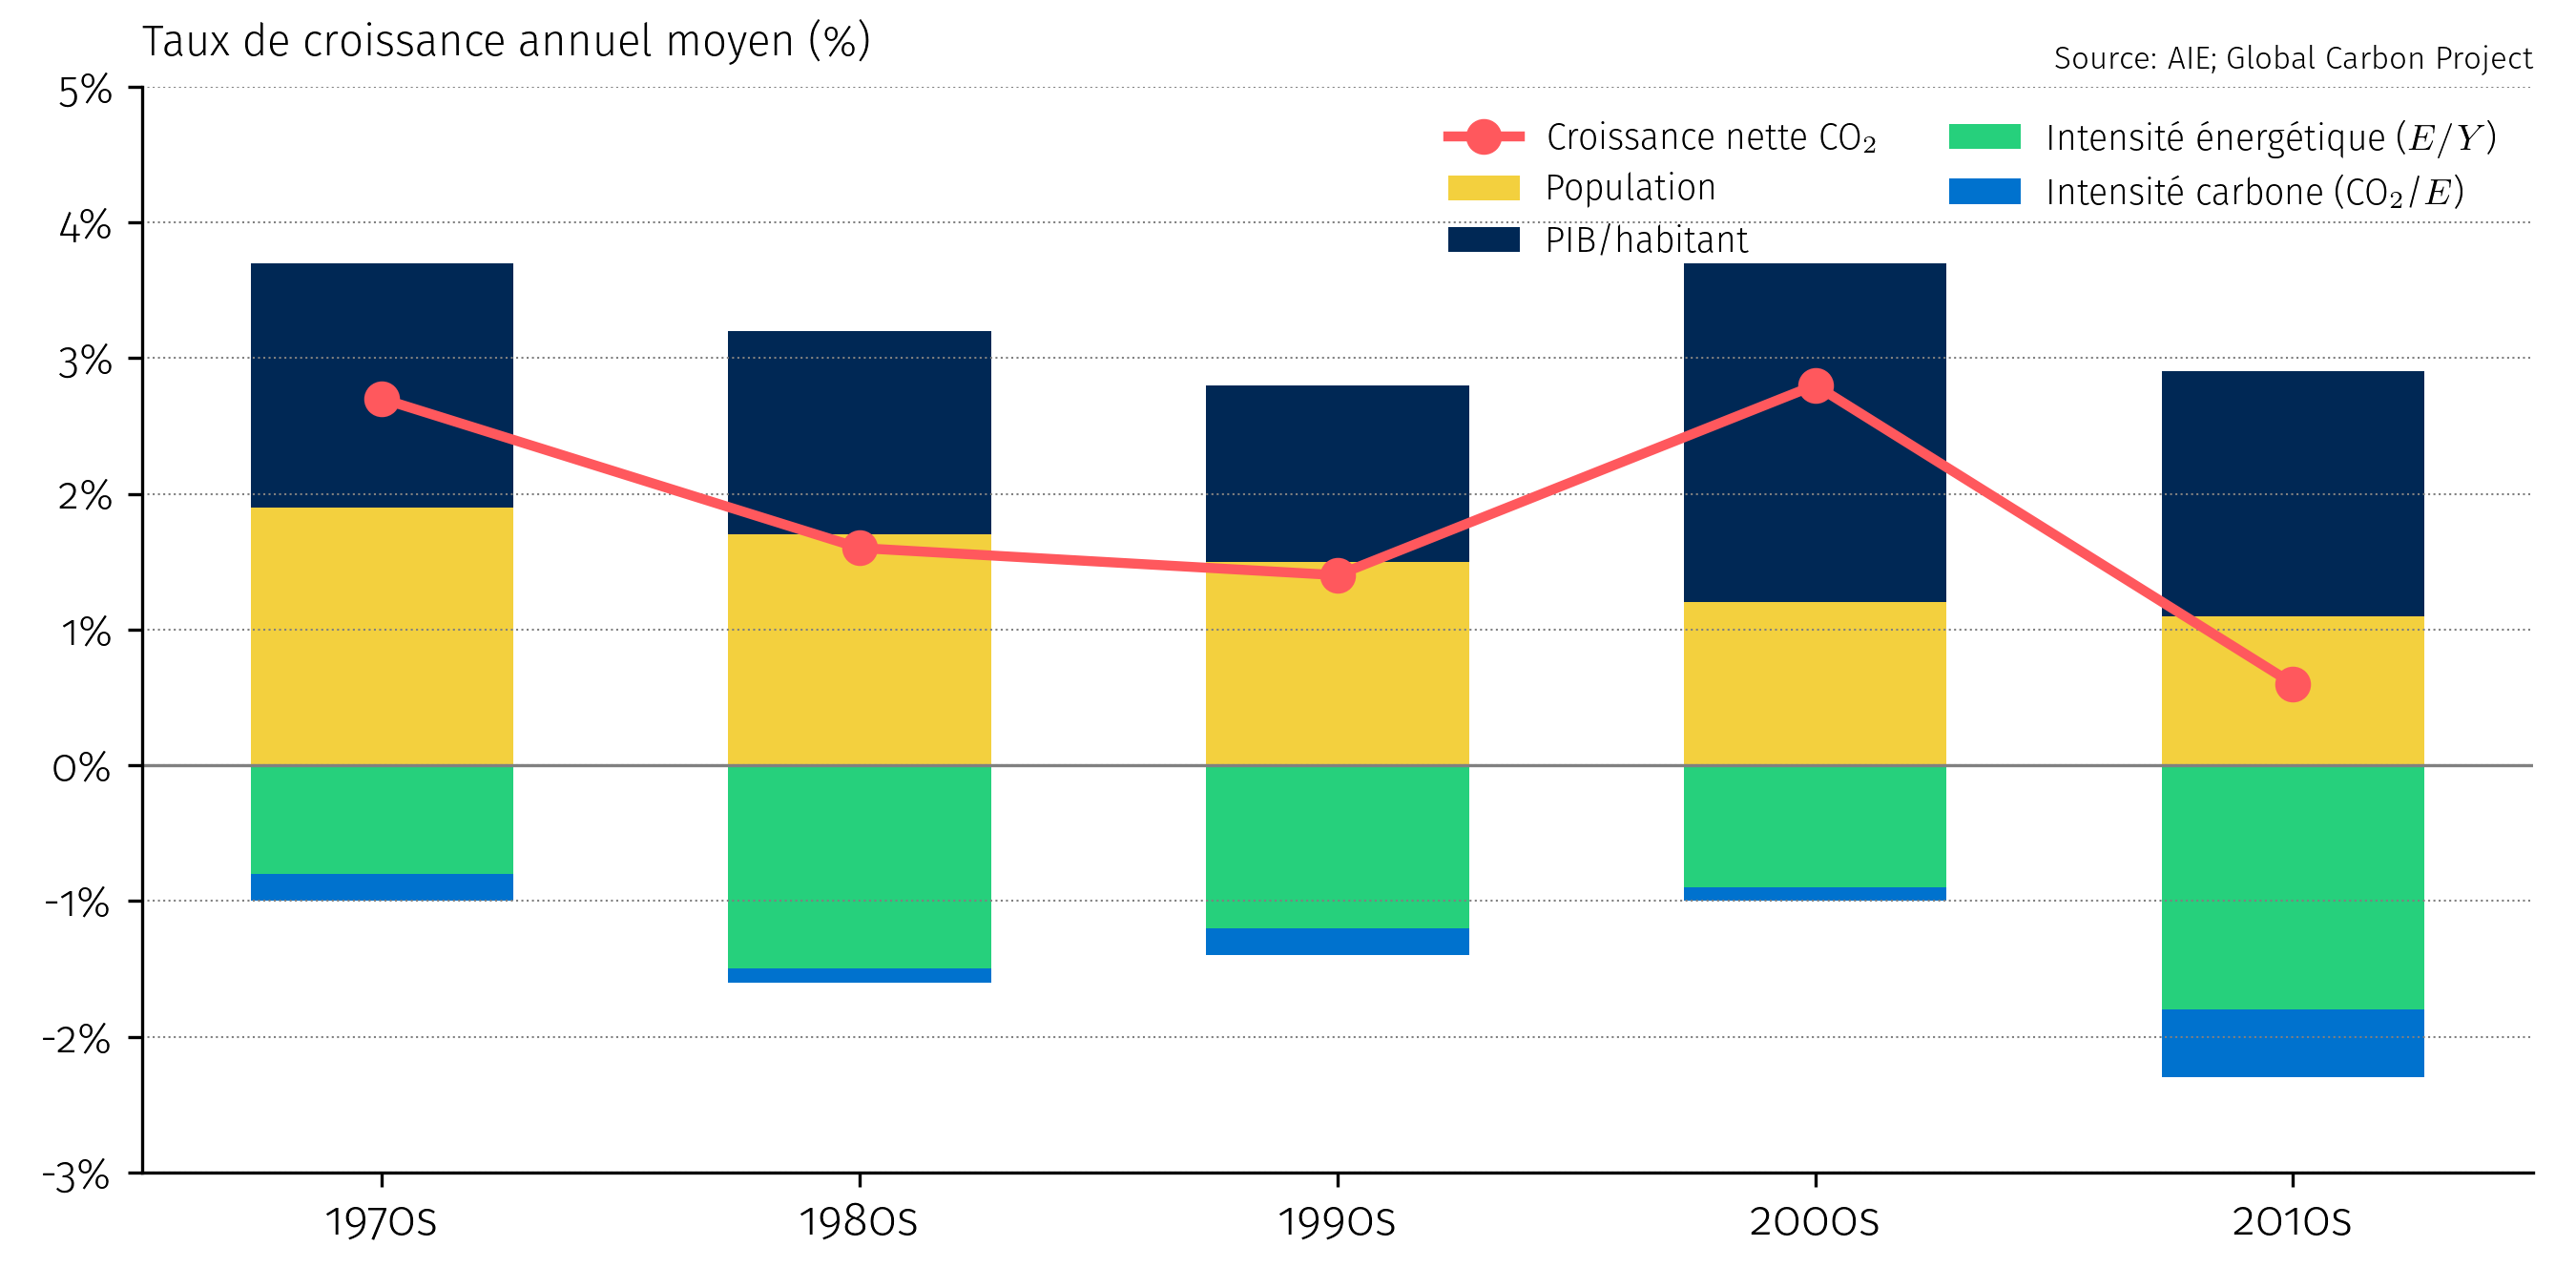
\includegraphics[width=0.95\textwidth]{kaya_decomposition.png}
   \end{figure}
\end{frame}

\begin{frame}[t]{Le découplage est-il possible?}
   \vspace{-0.2cm}
   \begin{figure}
      \centering
      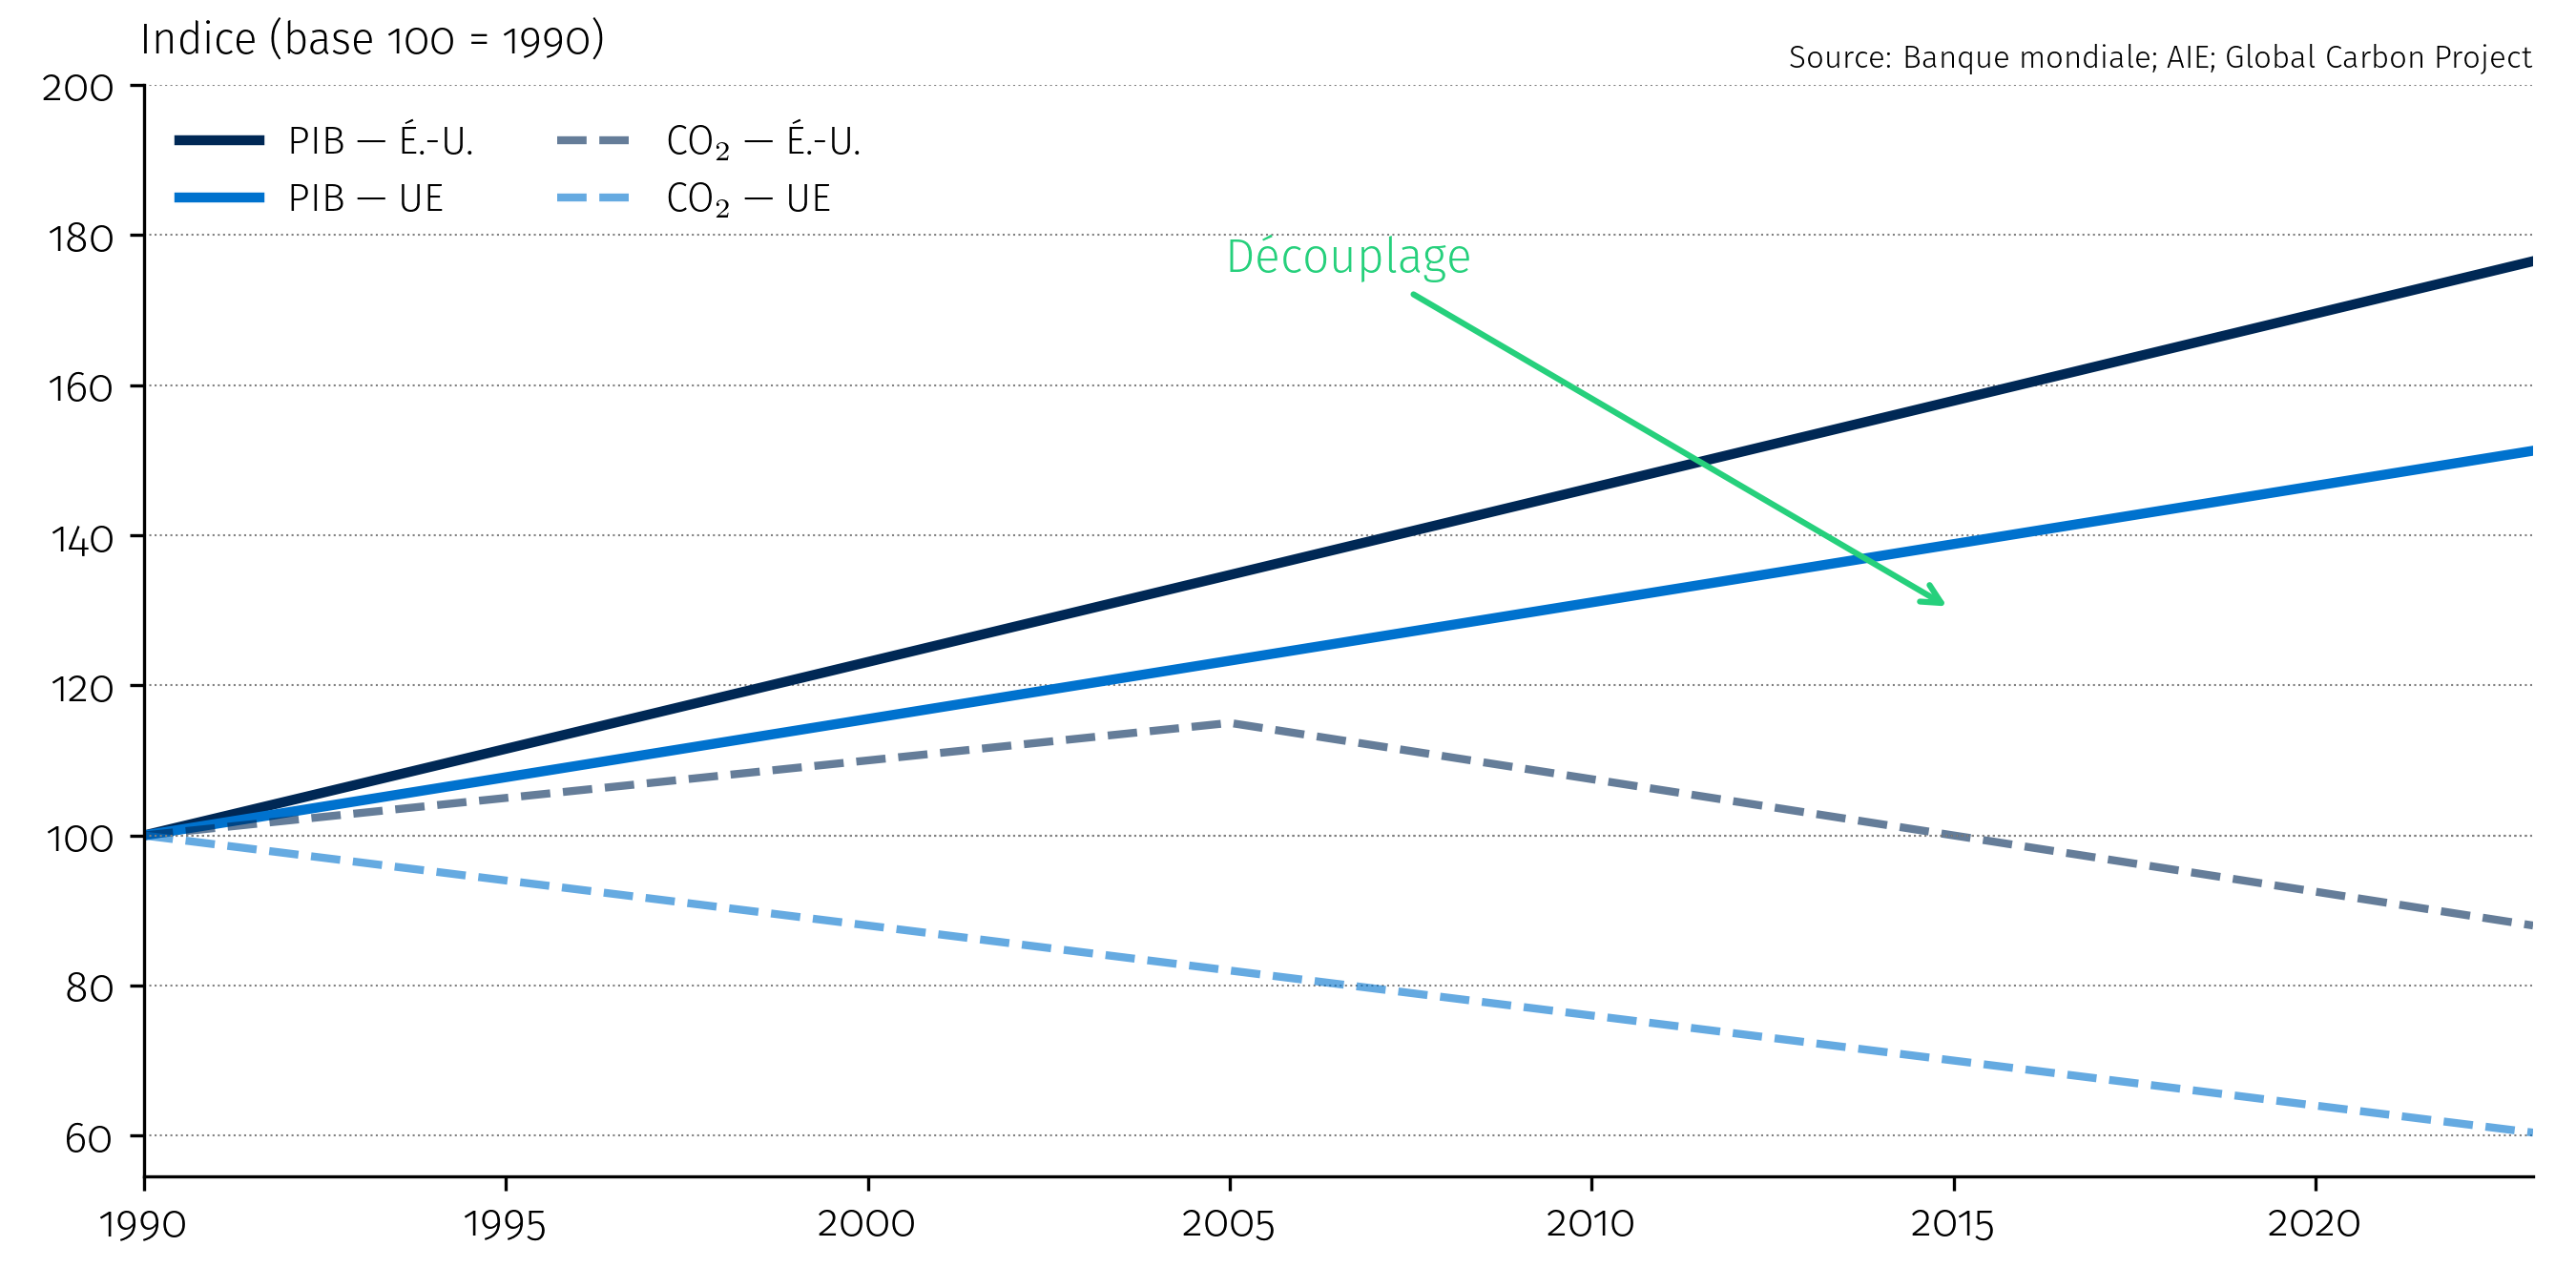
\includegraphics[width=0.85\textwidth, height=0.5\textheight, keepaspectratio]{decoupling.png}
   \end{figure}
   \vspace{-0.3cm}
   \begin{keyinsight}
      \small Croissance et baisse des émissions ne sont \textbf{pas incompatibles}. Mais le découplage exige que l'intensité énergétique et l'intensité carbone diminuent \textbf{plus vite} que le PIB n'augmente. C'est un défi technologique, pas une fatalité.
   \end{keyinsight}
\end{frame}

\begin{frame}[t]{Résumé}
   \footnotesize
   \begin{keyinsight}[Les leçons de la croissance de long terme]
      \begin{enumerate}
         \setlength\itemsep{0.08cm}
         \item L'accumulation de capital a des \textbf{limites} (rendements décroissants)
         \item Seule la \textbf{productivité} ($A$) peut soutenir une croissance indéfinie du niveau de vie
         \item Investir vous rend plus \textbf{riche}, mais ne vous fait pas croître plus \textbf{vite} indéfiniment
         \item Les \textbf{institutions} et les \textbf{idées} sont les déterminants profonds de la prospérité
         \item Le Canada souffre d'un déficit de productivité --- les solutions passent par l'\textbf{innovation}, pas seulement l'investissement physique
         \item La croissance soutenable requiert un \textbf{découplage} entre PIB et émissions (identité de Kaya)
      \end{enumerate}
   \end{keyinsight}
\end{frame}

% ============================================================================
\sectionframe{Avant la prochaine séance}
% ============================================================================

\begin{frame}[t]{Avant la prochaine séance}
   \textbf{Lectures suggérées :}
   \vspace{0.15cm}
   \begin{itemize}
      \setlength\itemsep{0.15cm}
      \item Acemoglu \& Robinson, \textit{Why Nations Fail} (chapitres 1--2)
      \item \textit{The Economist}, \guillemotleft~The productivity puzzle~\guillemotright
      \item OECD, \guillemotleft~Objectif croissance~\guillemotright, fiche Canada (2024)
   \end{itemize}
   \vspace{0.3cm}
   \textbf{Question de réflexion :}
   \vspace{0.15cm}

   \begin{tcolorbox}[
      colback=HECnavy!5, colframe=HECnavy, arc=8pt,
      leftrule=3pt, boxrule=0pt,
      left=10pt, right=10pt, top=6pt, bottom=6pt
   ]
      Le Canada peut-il relancer sa productivité \textbf{et} atteindre ses cibles climatiques? Utilisez l'identité de Kaya et le modèle de Solow pour structurer votre réponse.
   \end{tcolorbox}
   \vspace{0.3cm}
   \textbf{Prochaine séance :} Marché du travail, inégalités et IA
\end{frame}

\end{document}
